\listfiles
\documentclass[a4paper, 11pt,oneside]{book}

\usepackage{psl-cover}
\usepackage[headheight=14.5pt]{geometry}
\usepackage{imakeidx}
\makeindex[title = List of Definitions, intoc, options=-s index.ist]
\usepackage{epigraph}
\usepackage{fix-cm}
%Permits to copy eg x ⪰ y ⇔ v(x) ≥ v(y) from PDF to unicode data, and to search. From pdfTeX users manual. See https://tex.stackexchange.com/posts/comments/1203887.
	\input glyphtounicode
	\pdfgentounicode=1
%Latin Modern has more glyphs than Computer Modern, such as diacritical characters. fntguide commands to load the font before fontenc, to prevent default loading of cmr.
	\usepackage{lmodern}
%Encode resulting accented characters correctly in resulting PDF, permits copy from PDF.
	\usepackage[T1]{fontenc}
%UTF8 seems to be the default in recent TeX installations, but not all, see https://tex.stackexchange.com/a/370280.
	\usepackage[utf8]{inputenc}
	\usepackage{siunitx}
%Provides \newunicodechar for easy definition of supplementary UTF8 characters such as → or ≤ for use in source code.
	\usepackage{newunicodechar}
%Text Companion fonts, much used together with CM-like fonts. Provides \texteuro and commands for text mode characters such as \textminus, \textrightarrow, \textlbrackdbl.
	\usepackage{textcomp}
%St Mary’s Road symbol font, used for ⟦ = \llbracket.
	\usepackage{stmaryrd}
	\SetSymbolFont{stmry}{bold}{U}{stmry}{m}{n}
\usepackage[super]{nth}
\usepackage{centernot}
\usepackage{xpatch}
\usepackage{emptypage}
\usepackage[acronym,toc,automake,shortcuts]{glossaries}

\usepackage{caption}
\usepackage{subcaption}
\usepackage{booktabs}
\usepackage{graphicx}
\usepackage{times}
\usepackage{soul}
%\usepackage[hidelinks,hypertexnames=false]{hyperref}
\usepackage{xr}
\usepackage{dirtytalk}
\usepackage{fancyhdr}
\usepackage{paracol}
%Headers style
\pagestyle{fancy}
\fancyhead{}
\fancyhead[LE]{\scshape{Part~\thepart}, \leftmark}
%\fancyhead[LE]{\leftmark}% LE -> Left part on Even pages
\fancyhead[RO]{\rightmark}% RO -> Right part on Odd pages
%% remove the number at Conclusion

\makeatletter
\renewcommand\chaptermark[1]{
	\markboth{\textsc{%
			\ifnum\c@secnumdepth>\m@ne\if@mainmatter
			\@chapapp\ \thechapter. \ \fi\fi #1}}{}%
}
\makeatother

\appto\backmatter{
	\pagestyle{fancy}
	\fancyhead[LE,RO]{\leftmark}
} 


%chapter
\makeatletter
\def\thickhrulefill{\leavevmode \leaders \hrule height 1ex \hfill \kern \z@}
\def\@makechapterhead#1{%
	\vspace*{-30\p@}%
	{\parindent \z@ \raggedright \reset@font
		\scshape \@chapapp{} \thechapter
		\par\nobreak
		\interlinepenalty\@M
		\Huge  #1\par\nobreak
		%\vspace*{1\p@}%
		\hrulefill
		\par\nobreak
		\vskip 50\p@
}}
\def\@makeschapterhead#1{%
	\vspace*{-50\p@}%
	{\parindent \z@ \raggedright \reset@font
		\scshape \vphantom{\@chapapp{} \thechapter}
		\par\nobreak
		\interlinepenalty\@M
		\Huge  #1 \par\nobreak
		%\vspace*{1\p@}%
		\hrulefill
		\par\nobreak
		\vskip 30\p@
}}

%part
\makeatletter
\def\@part[#1]#2{%
	\ifnum \c@secnumdepth >-2\relax
	\refstepcounter{part}%
	\addcontentsline{toc}{part}{\thepart\hspace{1em}#1}%
	\else
	\addcontentsline{toc}{part}{#1}%
	\fi
	\markboth{}{}%
	\vspace*{-50\p@}%
	{\parindent \z@ \centering \reset@font
		\LARGE \scshape{Part \thepart}
		\par\nobreak
		\scshape \vphantom{\partname}
		\par\nobreak
		\interlinepenalty\@M
		\Huge  #1 \par\nobreak
		%\Huge \upshape \bfseries #1 \par\nobreak
		%\vspace*{1\p@}%
		\hrulefill
		\par\nobreak
		\vskip 30\p@
	}
		\kern-2pt
	\cleardoublepage
}
\makeatother



\usepackage{lipsum}


%ntheorem doc says: “empheq provides an enhanced vertical placement of the endmarks”; must be loaded before ntheorem. Loads the mathtools package, which loads and fixes some bugs in amsmath and provides \DeclarePairedDelimiter. amsmath is considered a basic, mandatory package nowadays (Grätzer, More Math Into LaTeX).
	\usepackage[ntheorem]{empheq}
%Package frenchb asks to load natbib before babel-french. Package hyperref asks to load natbib before hyperref.
	\usepackage{natbib}

%Turns the doi provided by some bibliography styles into URLs. However, uses old-style dx.doi url (see 3.8 DOI system Proxy Server technical details, “Users may resolve DOI names that are structured to use the DOI system Proxy Server (https://doi.org (current, preferred) or earlier syntax http://dx.doi.org).”, https://www.doi.org/doi_handbook/3_Resolution.html). The patch solves this.
	\usepackage{doi}
	\makeatletter
	\patchcmd{\@doi}{http://dx.doi.org}{https://doi.org}{}{}
	\makeatother
%Makes sure upper case greek letters are italic as well.
	\usepackage{fixmath}
%Provides \mathbb; obsoletes latexsym (see http://tug.ctan.org/macros/latex/base/latexsym.dtx). Relatedly, \usepackage{eucal} to change the mathcal font and \usepackage[mathscr]{eucal} (apparently equivalent to \usepackage[mathscr]{euscript}) to supplement \mathcal with \mathscr. This last option is not very useful as both fonts are similar, and the intent of the authors of eucal was to provide a replacement to mathcal (see doc euscript). Also provides \mathfrak for supplementary letters.
	\usepackage{amsfonts}
%Provides a beautiful (IMHO) \mathscr and really different than \mathcal, for supplementary uppercase letters. But there is no bold version. Alternative: mathrsfs (more slanted), but when used with tikzposter, it warns about size substitution, see https://tex.stackexchange.com/q/495167.
	\usepackage[scr]{rsfso}
%Multiple means to produce bold math: \mathbf, \boldmath (defined to be \mathversion{bold}, see fntguide), \pmb, \boldsymbol (all legacy, from LaTeX base and AMS), \bm (the most recommended one), \mathbold from package fixmath (I don’t see its advantage over \boldsymbol).
%“The \boldsymbol command is obtained preferably by using the bm package, which provides a newer, more powerful version than the one provided by the amsmath package. Generally speaking, it is ill-advised to apply \boldsymbol to more than one symbol at a time.” — AMS Short math guide. “If no bold font appears to be available for a particular symbol, \bm will use ‘poor man’s bold’” — bm. It is “best to load the package after any packages that define new symbol fonts” – bm. bm defines \boldsymbol as synonym to \bm. \boldmath accesses the correct font if it exists; it is used by \bm when appropriate. See https://tex.stackexchange.com/a/10643 and https://github.com/latex3/latex2e/issues/71 for some difficulties with \bm.
	\usepackage{bm}
%Also loaded by tikz.
	\usepackage{xcolor}
%Vizualization, on top of TikZ
	\usepackage{pgfplots}
	\pgfplotsset{compat=1.14}
	\usepackage{graphicx}
	\graphicspath{{graphics/}}
	\usepackage{tikz}
%	\usepackage[intoc]{acro}

\usepackage{hyperref}
\hypersetup{plainpages=false}

%Provides \print­length{length}, useful for debugging.
	%\usepackage{printlen}
	%\uselengthunit{mm}

\usepackage[capitalise]{cleveref}
%Do not use the displaymath environment: use equation. Do not use the eqnarray or eqnarray* environments: use align(*). This improves spacing. (See l2tabu or amsldoc.)
\let\proof\relax
\let\endproof\relax
\usepackage{amsthm}
%basic
\NewDocumentCommand{\R}{}{ℝ}
\NewDocumentCommand{\N}{}{ℕ}
%\mathscr is rounder than \mathcal.
\NewDocumentCommand{\powerset}{m}{\mathscr{P}(#1)}
%Powerset without zero.
\NewDocumentCommand{\powersetz}{m}{\mathscr{P}^*(#1)}
%https://tex.stackexchange.com/a/45732, works within both \set and \set*, same spacing than \mid (https://tex.stackexchange.com/a/52905).
\NewDocumentCommand{\suchthat}{}{\;\ifnum\currentgrouptype=16 \middle\fi|\;}
%Integer interval.
\NewDocumentCommand{\intvl}{m}{\llbracket#1\rrbracket}
%Allows for \abs and \abs*, which resizes the delimiters.
\DeclarePairedDelimiter\abs{\lvert}{\rvert}
\DeclarePairedDelimiter\card{\lvert}{\rvert}
%Perhaps should use U+2016 ‖ DOUBLE VERTICAL LINE here?
\DeclarePairedDelimiter\norm{\lVert}{\rVert}
%Better than using the package braket because braket introduces possibly undesirable space. Then: \begin{equation}\set*{x \in \R^2 \suchthat \norm{x}<5}\end{equation}.
\DeclarePairedDelimiter\set{\{}{\}}
\DeclarePairedDelimiter\ceil{\lceil}{\rceil}
\DeclarePairedDelimiter\floor{\lfloor}{\rfloor}

%Decision Theory (MCDA and SC)
\NewDocumentCommand{\allalts}{}{A}
\NewDocumentCommand{\allcrits}{}{\mathscr{C}}
\NewDocumentCommand{\alts}{}{A}
\NewDocumentCommand{\dm}{}{i}
\NewDocumentCommand{\allF}{}{\mathscr{F}}
\NewDocumentCommand{\allvoters}{}{\mathscr{N}}
\NewDocumentCommand{\voters}{}{N}
\NewDocumentCommand{\allprofs}{}{\boldsymbol{\mathcal{R}}}
\NewDocumentCommand{\prof}{}{P}
\NewDocumentCommand{\ibar}{}{\overline{i}}
\NewDocumentCommand{\lprof}{}{\lambda_P}
\NewDocumentCommand{\lprofi}{O{x}}{\lambda_P(#1)_i}
\NewDocumentCommand{\lprofibar}{O{x}}{\lambda_P(#1)_{\overline{i}}}
\NewDocumentCommand{\ineq}{}{(\sigma \circ \lambda_P)}

\NewDocumentCommand{\linors}{}{\mathcal{L}(\allalts)}
%Thanks to https://tex.stackexchange.com/q/154549
	%\makeatletter
	%\def\@myRgood@#1#2{\mathrel{R^X_{#2}}}
	%\def\myRgood{\@ifnextchar_{\@myRgood@}{\mathrel{R^X}}}
	%\makeatother
\NewDocumentCommand{\prefi}{O{i}}{\succ_{#1}}
\NewDocumentCommand{\paretopt}{}{\text{PO}}
\NewDocumentCommand{\SPPd}{}{\Sigma^\text{PPd}}
\NewDocumentCommand{\SAll}{}{\Sigma^\text{All}}
\NewDocumentCommand{\SThreshold}{}{\Sigma_\text{threshold}}
\NewDocumentCommand{\vpr}{}{\boldsymbol{v}}

\NewDocumentCommand{\musigma}{O{\sigma}O{P}}{\min_{A}({#1}\circ\lambda_{{#2}})}
\NewDocumentCommand{\mustar}{O{\sigma}O{P}}{\min_{\paretopt({#2})} ({#1} \circ \lambda_{#2})}
\NewDocumentCommand{\minineq}{O{\allalts}}{\min_{#1}(\sigma \circ \lambda)}
\NewDocumentCommand{\FBP}{}{\text{FB}(P)}
\NewDocumentCommand{\POP}{}{\text{PO}(P)}

\NewDocumentCommand{\alllosses}{}{\intvl{0, m-1}^N}

\NewDocumentCommand{\Ptop}{}{\bar{P}}
\NewDocumentCommand{\sigmatop}{}{\bar{\sigma}}
\NewDocumentCommand{\smad}{}{\sigma_\text{mad}}

\NewDocumentCommand{\fltwo}{}{\floor{\bar{l_2}}}
\NewDocumentCommand{\bltwo}{}{\bar{l_2}}

\newtheorem{conjecture}{Conjecture}
\newtheorem{example}{Example}
\newenvironment{abstract}{\rightskip1in\itshape}{}

\newtheorem{theorem}{Theorem}
\newtheorem{claim}{Claim}
\newtheorem{prop}{Proposition}
\newtheorem{corollary}{Corollary}
\newtheorem{definition}{Definition}
%\newtheorem{proof}{Proof}
\newtheorem{proposition}{Proposition}
\newtheorem{remark}{Remark}
%\newtheorem{sketch}[proof]{Proof Sketch}

%% generic theorem 

\newtheorem*{nonamethmplain}{\nonamethmname}
\theoremstyle{definition}
\newtheorem*{nonamethmdefinition}{\nonamethmname}
\theoremstyle{remark}
\newtheorem*{nonamethmremark}{\nonamethmname}
\newcommand{\nonamethmname}{}

\NewDocumentEnvironment{genthm}{O{plain}m}
{\vspace{0.2em}\renewcommand{\nonamethmname}{#2}\begin{nonamethm#1}}
	{{\footnotesize\qed} \end{nonamethm#1}}
\NewDocumentEnvironment{genthm*}{O{plain}mo}
{\renewcommand{\nonamethmname}{#2}%
	\IfNoValueTF{#3}
	{\begin{nonamethm#1}\relax}%
		{\begin{nonamethm#1}[#3]}%
			\mbox{}}
		{\end{nonamethm#1}}

	
\newtheoremstyle{indented}{3pt}{3pt}{\addtolength{\leftskip}{2.5em}}{}{\bfseries}{.}{\newline}{\thmname{#3}}
\theoremstyle{indented}
\newtheorem*{indented}{\nonamethmname}


%--------minimax-----
\DeclareMathOperator{\Regret}{Regret}
\DeclareMathOperator{\SCORE}{Score}
\DeclareMathOperator{\PMR}{PMR}
\DeclareMathOperator{\MaxR}{MR}
\DeclareMathOperator{\MMR}{MMR}
\DeclareMathOperator{\leximax}{leximax}
\DeclareMathOperator*{\argmax}{argmax}
\DeclareMathOperator*{\argmin}{argmin}

%Thanks to https://tex.stackexchange.com/q/154549
\makeatletter
\newcommand{\newrelation}[2]{% #1 = control sequence, #2 = replacement text
	\@ifdefinable{#1}{%
		\def#1{%
			\@ifnextchar_{\csname\string#1\endcsname}{\mathrel{#2}}%
		}%
		\@namedef{\string#1}##1##2{\mathrel{#2_{##2}}}%
	}%
}
\makeatother

\newrelation{\prefinc}{\!\parallel\!}%partial pref, complement (incomparable)
\newrelation{\pinc}{\bowtie^\text{p}}
%\newrelation{\prefinc}{Q^\text{p}}%partial pref, complement (incomparable)

\newcommand{\profile}{\bm{v}}%(complete) profile
\newcommand{\pprofile}{{\bm{p}}}%partial profile
\newcommand{\w}{\bm{w}}
\newcommand{\W}{\mathcal{W}}
\newcommand{\Co}{\mathcal{C}}
\newcommand{\pw}{W}%our knowledge about the weights
\newcommand{\strat}[1]{\emph{#1}}
\newcommand{\pref}{\succ}%real, connected pref, strict
\newcommand{\prefeq}{\succeq}%real, connected pref, strict
\newcommand{\prefr}{{\succ}^\text{r}}%real, connected pref, strict
\newcommand{\pprefeq}{\succeq^\text{p}}%partial pref
\newcommand{\ppref}{\succ^\text{p}}%partial pref
\newcommand{\pprefinv}{\prec^\text{p}}%partial pref
\newcommand{\nppref}{\nsucc^\text{p}}%negated partial pref


\newcommand{\oquot}{``}
\newcommand{\cquot}{''}

%Requires package xcolor.
\NewDocumentCommand{\commentOC}{m}{\textcolor{blue}{\small$\big[$OC: #1$\big]$}}
\NewDocumentCommand{\commentBN}{m}{\textcolor{magenta}{\small$\big[$BN: #1$\big]$}}
\NewDocumentCommand{\commentRS}{m}{\textcolor{red}{\small$\big[$RS: #1$\big]$}}

\bibliographystyle{abbrvnat}
\NewDocumentCommand{\possessivecite}{m}{\citeauthor{#1}’s \citeyearpar{#1}}

%https://tex.stackexchange.com/a/467188, https://tex.stackexchange.com/a/36088 - uncomment if one of those symbols is used.
%\DeclareFontFamily{U} {MnSymbolD}{}
%\DeclareFontShape{U}{MnSymbolD}{m}{n}{
%  <-6> MnSymbolD5
%  <6-7> MnSymbolD6
%  <7-8> MnSymbolD7
%  <8-9> MnSymbolD8
%  <9-10> MnSymbolD9
%  <10-12> MnSymbolD10
%  <12-> MnSymbolD12}{}
%\DeclareFontShape{U}{MnSymbolD}{b}{n}{
%  <-6> MnSymbolD-Bold5
%  <6-7> MnSymbolD-Bold6
%  <7-8> MnSymbolD-Bold7
%  <8-9> MnSymbolD-Bold8
%  <9-10> MnSymbolD-Bold9
%  <10-12> MnSymbolD-Bold10
%  <12-> MnSymbolD-Bold12}{}
%\DeclareSymbolFont{MnSyD} {U} {MnSymbolD}{m}{n}
%\DeclareMathSymbol{\ntriplesim}{\mathrel}{MnSyD}{126}
%\DeclareMathSymbol{\nlessgtr}{\mathrel}{MnSyD}{192}
%\DeclareMathSymbol{\ngtrless}{\mathrel}{MnSyD}{193}
%\DeclareMathSymbol{\nlesseqgtr}{\mathrel}{MnSyD}{194}
%\DeclareMathSymbol{\ngtreqless}{\mathrel}{MnSyD}{195}
%\DeclareMathSymbol{\nlesseqgtrslant}{\mathrel}{MnSyD}{198}
%\DeclareMathSymbol{\ngtreqlessslant}{\mathrel}{MnSyD}{199}
%\DeclareMathSymbol{\npreccurlyeq}{\mathrel}{MnSyD}{228}
%\DeclareMathSymbol{\nsucccurlyeq}{\mathrel}{MnSyD}{229}
%\DeclareFontFamily{U} {MnSymbolA}{}
%\DeclareFontShape{U}{MnSymbolA}{m}{n}{
%  <-6> MnSymbolA5
%  <6-7> MnSymbolA6
%  <7-8> MnSymbolA7
%  <8-9> MnSymbolA8
%  <9-10> MnSymbolA9
%  <10-12> MnSymbolA10
%  <12-> MnSymbolA12}{}
%\DeclareFontShape{U}{MnSymbolA}{b}{n}{
%  <-6> MnSymbolA-Bold5
%  <6-7> MnSymbolA-Bold6
%  <7-8> MnSymbolA-Bold7
%  <8-9> MnSymbolA-Bold8
%  <9-10> MnSymbolA-Bold9
%  <10-12> MnSymbolA-Bold10
%  <12-> MnSymbolA-Bold12}{}
%\DeclareSymbolFont{MnSyA} {U} {MnSymbolA}{m}{n}
%%Rightwards wave arrow: ↝. Alternative: \rightsquigarrow from amssymb, but it’s uglier
%\DeclareMathSymbol{\rightlsquigarrow}{\mathrel}{MnSyA}{160}

%03B3 Greek Small Letter Gamma
\newunicodechar{γ}{\gamma}
%03B4 Greek Small Letter Delta
\newunicodechar{δ}{\delta}
%2115 Double-Struck Capital N
\newunicodechar{ℕ}{\mathbb{N}}
%211D Double-Struck Capital R
\newunicodechar{ℝ}{\mathbb{R}}
%21CF Rightwards Double Arrow with Stroke
\newunicodechar{⇏}{\nRightarrow}
%21D2 Rightwards Double Arrow
\newunicodechar{⇒}{\ensuremath{\Rightarrow}}
%21D4 Left Right Double Arrow
\newunicodechar{⇔}{\Leftrightarrow}
%21DD Rightwards Squiggle Arrow
\newunicodechar{⇝}{\rightsquigarrow}
%2212 Minus Sign
\newunicodechar{−}{\ifmmode{-}\else\textminus\fi}
%2227 Logical And
\newunicodechar{∧}{\land}
%2228 Logical Or
\newunicodechar{∨}{\lor}
%2229 Intersection
\newunicodechar{∩}{\cap}
%222A Union
\newunicodechar{∪}{\cup}
%2260 Not Equal To (handy also as text in informal writing)
\newunicodechar{≠}{\ensuremath{\neq}}
%2264 Less-Than or Equal To
\newunicodechar{≤}{\leq}
%2265 Greater-Than or Equal To
\newunicodechar{≥}{\geq}
%2270 Neither Less-Than nor Equal To
\newunicodechar{≰}{\nleq}
%2271 Neither Greater-Than nor Equal To
\newunicodechar{≱}{\ngeq}
%2272 Less-Than or Equivalent To
\newunicodechar{≲}{\lesssim}
%2273 Greater-Than or Equivalent To
\newunicodechar{≳}{\gtrsim}
%2274 Neither Less-Than nor Equivalent To – also, from MnSymbol: \nprecsim, a more exact match to the Unicode symbol; and \npreccurlyeq, too small
\newunicodechar{≴}{\not\preccurlyeq}
%2275 Neither Greater-Than nor Equivalent To
\newunicodechar{≵}{\not\succcurlyeq}
%2279 Neither Greater-Than nor Less-Than – requires MnSymbol; also \nlessgtr from txfonts/pxfonts, \ngtreqless from MnSymbol (but much higher), \ngtrless from MnSymbol (a more exact match to the Unicode symbol); for incomparability (not matching this Unicode symbol), may also consider \ntriplesim from MnSymbol,\nparallelslant from fourier, \between from mathabx, or ⋈
\newunicodechar{≹}{\ngtreqlessslant}
%227A Precedes
\newunicodechar{≺}{\prec}
%227B Succeeds
\newunicodechar{≻}{\succ}
%227C Precedes or Equal To
\newunicodechar{≼}{\preccurlyeq}
%227D Succeeds or Equal To
\newunicodechar{≽}{\succcurlyeq}
%227E Precedes or Equivalent To
\newunicodechar{≾}{\precsim}
%227F Succeeds or Equivalent To
\newunicodechar{≿}{\succsim}
%2280 Does Not Precede
\newunicodechar{⊀}{\nprec}
%2281 Does Not Succeed
\newunicodechar{⊁}{\nsucc}
%22B2 Normal Subgroup Of – using \vartriangleleft from amsfonts, which goes well with \trianglelefteq, \ntriangleright, and so on, also from amsfonts; another possibility is \lhd from latexsym, which seems visually equivalent to \vartriangleleft from amsfonts; latexsym also has ⊴=\unlhd, but doesn’t have a symbol for ⊴. Other related symbols: \triangleleft from latesym package is too small; fdsymbol provides \triangleleft=\medtriangleleft and \vartriangleleft=\smalltriangleleft; MnSymbol provides \medtriangleleft and \vartriangleleft=\lessclosed=\lhd which are smaller than \vartriangleleft from amsfont; \vartriangleleft from mathabx (p. 67), looks different (wider); also \vartriangleleft from boisik (p. 69) looks still different; \vartriangleleft=\lhd from stix are smaller. Oddly enough, \triangleright appears as the LMMathItalic12-Regular font whereas \rhd appears as LASY10 and \vartriangleright appears as MSAM10.
\newunicodechar{⊲}{\vartriangleleft}
%22B3 Contains as Normal Subgroup (also: 25B7 White right-pointing triangle or 25B9 White right-pointing small triangle)
\newunicodechar{⊳}{\vartriangleright}
%22B4 Normal Subgroup of or Equal To
\newunicodechar{⊴}{\trianglelefteq}
%22B5 Contains as Normal Subgroup or Equal To
\newunicodechar{⊵}{\trianglerighteq}
%22C8 Bowtie
\newunicodechar{⋈}{\bowtie}
%22EA Not Normal Subgroup Of
\newunicodechar{⋪}{\ntriangleleft}
%22EB Does Not Contain As Normal Subgroup
\newunicodechar{⋫}{\ntriangleright}
%22EC Not Normal Subgroup of or Equal To
\newunicodechar{⋬}{\ntrianglelefteq}
%22ED Does Not Contain as Normal Subgroup or Equal
\newunicodechar{⋭}{\ntrianglerighteq}
%25A1 White Square
\newunicodechar{□}{\Box}
%27E6 Mathematical Left White Square Bracket – requires stmaryrd (alternative: \text{\textlbrackdbl}, but ugly if used in an italicized text such as a theorem)
\newunicodechar{⟦}{\llbracket}
%27E7 Mathematical Right White Square Bracket
\newunicodechar{⟧}{\rrbracket}
%27FC Long Rightwards Arrow from Bar
\newunicodechar{⟼}{\longmapsto}
%2AB0 Succeeds Above Single-Line Equals Sign
\newunicodechar{⪰}{\succeq}
%301A Left White Square Bracket
\newunicodechar{〚}{\textlbrackdbl}
%301B Right White Square Bracket
\newunicodechar{〛}{\textrbrackdbl}
%→ is defined by default as \textrightarrow, which is invalid in math mode. Same thing for the three other commands. Using \DeclareUnicodeCharacter instead of \newunicodechar because the latter warns about the previous definition.
%→ Rightwards Arrow
\DeclareUnicodeCharacter{2192}{\ifmmode\rightarrow\else\textrightarrow\fi}
%¬ Not Sign
\DeclareUnicodeCharacter{00AC}{\ifmmode\lnot\else\textlnot\fi}
%… Horizontal Ellipsis
\DeclareUnicodeCharacter{2026}{\ifmmode\dots\else\textellipsis\fi}
%× Multiplication Sign
\DeclareUnicodeCharacter{00D7}{\ifmmode\times\else\texttimes\fi}
%Permits to really obtain a straight quote when typing a straight quote; potentially dangerous, see https://tex.stackexchange.com/a/521999
%\catcode`\'=\active
%\DeclareUnicodeCharacter{0027}{\ifmmode{^{\prime}}\else\textquotesingle\fi}

%\newcommand{\cmark}{\ding{51}}%
%\newcommand{\xmark}{\ding{53}}
\newglossaryentry{scr}
{
    name=Social Choice Rule,
    description={Social Choice Rule is is a mapping $f:\linors^{N}\rightarrow 2^{A} \setminus \{\emptyset \}$}
}

%\DeclareAcronym{SCR}{short=SCR, long={Social Choice Rule}}

\newacronym{SCR}{SCR}{Social Choice Rule}
\title{Compromise and elicitation in social choice: a study of egalitarianism and incomplete information in voting}

\author{Beatrice NAPOLITANO}

\institute{l'Université Paris-Dauphine}
\doctoralschool{École Doctorale SDOSE}{543}
\specialty{Informatique}
\date{09 Décembre 2022}


%\jurymember{7}{Prénom NOM}{Titre, établissement}{Président}
\jurymember{1}{Olivier CAILLOUX}{MdC, Université Paris-Dauphine}{Examinateur}
\jurymember{2}{Ayça EBRU GIRITLIGIL}{MdC, İstanbul Bilgi University}{Examinatrice}
\jurymember{3}{Vincent MOUSSEAU}{Professeur, CentraleSupélec Université Paris-Saclay\vspace{0.3cm}}{Rapporteur}
\jurymember{4}{İpek ÖZKAL SANVER}{Professeure, İstanbul Bilgi University}{Rapporteuse}
\jurymember{5}{Remzi SANVER}{Directeur de recherche, CNRS Université Paris-Dauphine\vspace{0.3cm}}{Directeur de thèse}
\jurymember{6}{Paolo VIAPPIANI}{Chargé de Recherche, Université Paris-Dauphine\vspace{0.3cm}}{Examinateur}


%moins de 1000 caractères
%This is 1760
\frabstract{
	Les règles de vote représentent des moyens formels d'agréger les préférences d'un groupe d'électeurs en une décision collective. Mais quelle règle choisir dépend du contexte et de la conception de la justice de la société concerné.
	Bien que toutes les règles de vote puissent être considérées comme un compromis entre individus, certaines le sont plus que d'autres.
	Dans ce manuscrit, nous proposons deux définition de compromis basées sur une notion de <<equal-loss>>, favorisant un résultat où chaque électeur concède le plus également possible.
	Nous étudions plusieurs règles qui reflètent un certain concept de compromis et nous montrons comment, bien qu'elles imposent une volonté de compromis aux individus, elles ne garantissent pas un résultat où chacun a effectivement concédé.
	De plus, nous remettons en question l'hypothèse, souvent faite dans le cadre classique, que la règle de vote est fixée à l'avance et qu'une information complète sur les préférences des individus est fournie. En nous concentrant sur les règles de vote positionnelle, nous proposons des procédures d'élicitation capables de poser des questions aux votants et à l'entité responsable de la conception de la règle de vote, afin d'obtenir rapidement les informations les plus pertinentes.
	En considérant la règle de Jugement Majoritaire, nous analysons une procédure d'élicitation des préférences utilisée dans des scénarios de vote réels. Sur la base d'une information partielle sur les préférences des individus, nous analysons la probabilité de sélectionner un gagnant différent de celui obtenu en considérant le profil complet et nous étudions le nombre minimum de questions à poser aux électeurs pour que cette probabilité soit faible.
}

%moins de 1000 caractères
%This is 1581
\enabstract{
	Voting rules are formal means of aggregating preferences of a group of voters over a set of alternatives into a collective decision. But which rule to use is a difficult question and the answer depends on the conception of justice of the concerned society or committee. 
	Although all voting rules can be seen as a compromise between individuals, some are more so than others.
	In this manuscript we provide two notions of compromise based on an equal-loss perspective, favoring an outcome where every voter concedes as equally as possible. We study several rules that reflect some idea of compromise and show how, although imposing a willingness to compromise on individuals, they fail to ensure an outcome where everyone has effectively compromised.	
  	Moreover, we question the assumption, often made in the classical setting, that the voting rule is fixed beforehand and full information on the preferences of the individuals is provided. Focusing on positional scoring rules, we propose elicitation procedures based on minimax regret, able to interleave questions to the voters and to the entity responsible for designing the voting rule in order to quickly obtain the most relevant information.
  	Considering \acl{MJ} rule, we analyze a particular preference elicitation procedure used in real voting scenarios. Given a partial information on individuals preferences, we analyze the probability of selecting a different winner from the one obtained by considering the full profile and study the minimum number of questions to ask voters in order for this probability to be low.
}

\frkeywords{Intelligence Artificielle, Computational Social Choice, Théorie de la décision, Élicitation de préférence, Modélisation des préférences.}
\enkeywords{Artificial Intelligence, Computational Social Choice, Decision Theory, Preference Elicitation, Preference Modeling.}


\makeglossaries
%\hypersetup{draft}
\begin{document}

\hypersetup{pageanchor=false}
\begin{titlepage}
\maketitle{}
\end{titlepage}

\frontmatter

\begingroup
\hypersetup{hidelinks}

\tableofcontents

\listoffigures
\addcontentsline{toc}{chapter}{List of Figures}

\listoftables
\addcontentsline{toc}{chapter}{List of Tables}

\endgroup

\printglossary[toctitle=List of Abbreviations,title=List of Abbreviations,type=\acronymtype]

\mainmatter

\part{Introduction} 

	\chapter{Introduction}
		\label{ch:intro}
		%!TeX root=../thesis.tex
\setlength\epigraphwidth{.7\textwidth}
\setlength\epigraphrule{0pt}
\renewcommand{\textflush}{flushepinormal}
%\renewcommand{\sourceflush}{flushright}
\epigraph{\itshape Democracy is difficult, flawed and unstable. It involves barely distinguishable political parties taking part in lengthy, over-complicated and expensive decision-making processes. Trying to engage so many people with political issues seems to lead only to complexity and disagreement. So why bother?}{--- Michela Murgia, \textit{Istruzioni per diventare fascisti}\\ \scriptsize{(Trans. \textit{How to be a Fascist: A Manual} by Alex Valente)}}


Collective decision-making is a process in which individual preferences are aggregated to form a single group choice. This broad definition allows to consider instances that seem very different from each other.
Some examples include \textit{fair allocation problems}\textemdash which address the problem of fairly dividing some resources among individuals who have different interests in such resources, e.g. houses allocation, creation of a working schedule etc.\textemdash 
\textit{matching problems}\textemdash which deal with the problem of matching individuals from two separate groups considering their preferences, e.g. students to schools, tenants to houses etc.\textemdash 
and \textit{judgment aggregation problems}\textemdash whose solutions try to group the beliefs of different individuals into a judgment that reflects the society as a single entity.
In this thesis we will focus on another example of collective decision-making: \textit{voting}. Given a set of individuals who express their preferences over a given set of candidates, how do we select the \textit{best} candidate for the group? This is a very ancient dilemma that has been faced multiple times during centuries and that we are going to tackle throughout this manuscript.
As we shall see, the answer depends on many factors, such as the information we have at our disposal \textemdash do we know the preferences of all voters with respect to all candidates? \textemdash and the properties we want the outcome to satisfy \textemdash what do we mean by the best candidate? Who decides what is best?

An important methodology in our work is to define desirable properties we want a rule to satisfy. This allows us, on one hand, to divide aggregation rules into classes of methods satisfying the same properties, and, on the other hand, to do the inverse process: starting from an already defined method to help the decision-maker understand its properties.
The lack of information and the assistance to decision-makers are two of the themes explored in the course of this work.

This introductory chapter aims to introduce the contributions and organization of this dissertation, but also, and maybe more importantly, to introduce its motives.
We have mentioned the analysis of aggregation processes through the definition of desiderata, but this axiomatic approach is very recent and started only after the publication of the Ph.D. thesis of Kenneth \citet{Arrow1951}.
However, the theory behind collective decision-making processes is much older and, as \citet{McLean1990} wrote, \say{the theory of voting is known to have been discovered three times and lost twice}. To understand what we are studying today, we think it is essential to take a look at the past.
Starting from the first traces of decision-making processes in history, we consider early voting mechanisms that focused mainly on particular cases.
From the analysis of specific instances, we move on to the start of \textit{Social Choice Theory} as a formal scientific discipline.
We then focus on how it has managed to evolve by incorporating computational aspects typical of the computer science field.
Finally, we discuss how this led us to investigate the problems that will be described in the following chapters and we outline our contributions.

\section{Voting rules from practice to theory}
The first records of collective choice problems can be traced back to ancient Greece (ca. 500 BC), and the word democracy itself originated from the greek dēmokratiā: dēmos \textit{people} and kratos \textit{rule}.
Many scholars, including Aristotle, have described in details the functioning of Athenian democratic institutions, however they never formally analysed voting processes. This appears to be partly due to the fact that Athenian voters where asked to express their preferences over only two alternatives: the choices were often in the form of \textit{yes/no}, \textit{banish/not banish} \citep{McLeanUrken1995}.
\paragraph{From ancient Rome to the Middle Ages: the precursors of social choice.}
Today we know that most of the problems in social choice arise when at least three alternatives are considered.
Exactly this reason brought Pliny the Younger, a magistrate of Ancient Rome, to write a letter to his jurist friend Titius Aristo (105 AD). In the letter, that can be found translated in \citet[Chapter 2]{McLeanUrken1995}, Pliny asks Titius advice about a problem that emerged during a vote in the Senate. 
A consul had been found dead and his servants were suspected of his death, the Senate had to decide whether to free them, to banish them or to put them to death. For the first time they were facing a problem with more than two choices and, with it, its related issues.
Pliny explains that the first option was acclaimed by the largest number of senators but not by the majority of them. Thus, he asked the Senate to consider the alternatives as three separate ones on the principle of huge disparity in punishments, and tried to arrange a series of binary votes among the three verdicts.
Pliny was aware of his own attempt to manipulate the elections in favor of his top choice, freeing the slaves, but so was one of his adversary, supporter of the death penalty.
The latter knew that the most lenient sentence would have won in binary votes against banishment and death taken separately, so he withdraw his proposal that could not have defeated any of the others.
The supporters of death penalty then moved their support to banishment that easily won, having now a strong majority. Note how by changing the way we aggregate the same set of preferences we can have completely different outcomes.

Pliny's concern shows how some desiderata of electoral protocols are not only restricted to modern society. The desire for a transparent system that was difficult to manipulate was present also in medieval elections. However, after Pliny, the democratic process did not find much room in the public discussion. The only two exceptions of abstract works on voting rules in the Middle Ages were the ones of Ramon Llull (ca. 1232-1316) and Nicolaus Cusanus (1401-1464). The lack of theoretic analysis led to the creation of overly complicated electoral processes in order to make manipulations so difficult as to be impossible in practice \citep{Uckelman2010}. For example, Venice's 1268 ordinance, which described the procedure to elect the Doge (the head of the state), involved nine stages from the elections of the first committee to the election of the Doge himself. The procedure, discussed in detail by \citet{Lines1986, Coggins1998, Mowbray2007} can be summarized by this folk poem \citep[p.79]{Doglioni1666}:
\vspace{1em}
\begin{paracol}{2}
	\begin{leftcolumn}
		\centering
		\textit{\say{Trenta elegge il conseglio. \\ 
			Di quei nove hanno il meglio; \\
			Questi eleggon quaranta; \\
			Ma chi di lor si vanta \\
			Son dodici che fanno \\
			Venticinque: ma stanno \\
			Di questi solo nove \\
			Che fan con le lor prove \\
			Quarantacinque a ponto \\
			De’ quali undici in conto, \\
			Eleggon quarantuno, \\
			Che chiusi tutti in uno, \\
			Con venticinque almeno \\
			Voti, fanno il sereno \\
			Principe che corregge \\
			Statuti, ordini e legge.}}
	\end{leftcolumn}
	
	\begin{rightcolumn}
		\centering
			Thirty elect the board. \\ 
			Of those, nine prevail. \\
			These elect forty.\\
			But those of them who brag \\
			are twelve, that elect \\
			twenty-five: of these \\
			only nine remain; \\
			who make with their evidence \\
			forty-five in total. \\
			Of those, eleven \\
			elect forty-one, \\
			who closed all together, \\
			with at least twenty-five \\
			votes, make the serene \\
			Prince who corrects \\
			articles, orders and laws. \\
	\end{rightcolumn}
\end{paracol}
\vspace{2em}

\citet{Wolfson1899} and \citet{Keller2014} describe more electoral processes in Italian communes. 

At the end of the thirteenth century Ramon Llull designed and discussed two voting methods in his works: \textit{Artifitium electionis personarum} [ca. 1274-83] (The method of the election of persons), \textit{En qual manera Natana fo eleta a abadessa} [ca. 1283] (In which way that Natana was elected abbess which corresponds to the 24th chapter of his novel \textit{Blaquerna}), and \textit{De arte eleccionis} [1299] (On the method of election). \cite{Hagele2001} present the original texts together with their English translation. Llull was a Catalan missionary and philosopher, and he was particularly interested in ecclesiastic elections. In the first two works we cited, Llull describes a precise schema of comparisons between each pair of candidates. The candidate winning the largest number of pairwise comparison was selected as a winner. The last method, described in \textit{De arte eleccionis}, is also based on pairwise comparisons but with a system of successive eliminations. The candidate winning the last comparison was selected as a winner. While the first two methods can be viewed as equivalent to either a Condorcet's method or a Borda count depending on the interpretation of Llull's text, the third method is a Condorcet's procedure \citep{McLean1990}. A candidate is the Condorcet winner if she beats every other candidate in pairwise comparisons. A voting rule is a Condorcet procedure if it elects the Condorcet winner whenever it exists.

Unfortunately, his works have not received much attention, except from Nicolas Cusanus, a German theologian and philosopher who studied Llull's \textit{De arte eleccionis}. He rejected Llull's work and proposed his own voting procedure in a chapter of his work \textit{De concordantia catholica} [ca. 1431-34] (Catholic concordance), which can be found in \citet[Chapter 4]{McLeanUrken1995}. Cusanus' main concern was to reduce manipulation and strategic voting and he recommended a Borda count method with secrete voting. We must say that there are no evidence that Cusanus was aware of the other two methods proposed by Llull, but only of the Condorcet-like one. With this in mind, we can see that although both Llull and Cusanus wanted to reduce manipulation, the methods they proposed turned out to be quite different.
This is probably due to the different contexts they were considering. Llull had in mind an election where members of an abbey had to select their own leader: voters were people who knew and trusted each other and would have lived together even after the vote. Cusanus, on the other hand, wrote \textit{De concordantia catholica} while attending the Council of Basel: voters were people that would have met only once to elect the new head of the Catholic Church and had their own interests and strategies. This underlines a very important point about voting methods: context matters. If we were to define a voting procedure, the first thing to consider is \say{to elect what?}.
\paragraph{Enlightenment and the revival of choice.}
To find new discussions on voting procedures we must skip the rest of the Middle Ages and move on to the Enlightenment. In particular, we must travel to the France of the late eighteenth century. This should come as no surprise since in France sciences had been extremely well organized for at least a century through the establishment of the \say{Académie royale des sciences} by Louis XIV in 1666 \citep{Demeulenaere1995}. Starting from 1753 membership to the Academy was decided through elections using plurality rule and in 1770 Jean-Charles de Borda argued that this method could lead to undesirable results. In particular, he showed how the candidate elected under plurality could lose in case of pairwise comparisons, and he proposed instead a rank order count \textemdash what we now call Borda count which is also equivalent to the Cusanus method. Although Borda presented these observations to the Academy in 1770, elections continued to be conducted using plurality rule and his work was published many years later \citep{Borda1784}.
One of the reasons for this delay has been attributed to one of his political opponents: Nicolas de Condorcet \citep{Urken2004} \textemdash also known as Marquis of Condorcet. In fact, the latter had meanwhile become secretary of the Academy, presumably also thanks to the voting method in place, and was responsible for scheduling publications. %Borda was an ardent supporter of absolute monarchy
The year after the publication of Borda's method, the Marquis of Condorcet also proposed a voting procedure, the one we now recognise as equivalent to LLull's method \citep{Condorcet1785}.
After the revolution, the Academy was reformed into the so-called \say{Institut de France} and Napoleon appointed a commission to study the voting mechanisms to be used within it. The commission chose Borda's method but after a while Napoleon took the unilateral decision to switch back to the use of plurality.

Once again, all these works were ignored until the second half of the 20th century. One of the few noteworthy works is that of Charles Dogson, better known as Lewis Carroll. Although not aware of the studies of the Marquis of Condorcet, in 1876 he proposed a voting procedure that solves the paradox arising in the Condorcet method when cycles occur.
In his proposition the winner is the only candidate that wins every pairwise comparison (Condorcet winner). If such a candidate does not exist then for each candidate we count the number of changes in the voter preferences required for they to be the Condorcet winner. The elected candidate is the one associated to the lowest number of changes.
\paragraph{The axiomatization of social choice theory.}
This concludes a brief introduction to the start of voting theory which has so far been concerned with analysing procedures, and their related problems, on the basis of examples. From this point on, and especially since the publication of the Ph.D. thesis of Kenneth \citet{Arrow1951}, social choice theory emerges as a scientific discipline. Arrow, in fact, was the first to introduce axiomatic analysis of aggregation methods and to characterize classes of rules on the basis of the set of properties they satisfy. In his thesis, he also defines a small set of axioms that seem naturally desirable and then he proves that the only voting rule able to satisfy them all is the dictatorship. This opened the door to the research that followed over the next sixty years.

In the meantime, however, the aforementioned works were still unknown to the general public, until a few years later, when Duncan \citet{Black1958} published the book that soon became the basis of Social Choice Theory: \textit{The Theory of Committees and Elections}. From this point onwards, new axioms are recurrently proposed and new electoral rules analysed. We will describe the most relevant ones to this work in the next chapter.

For reasons of space, and complexity of the topic, many authors who have worked on electoral procedures \textemdash e.g. Pufendorf, Daunou, LaPlace, Lhulier, Nanson, Galton, Scitovsky, Bergson, Samuelson etc.\textemdash have not been mentioned in this chapter. More details on the history of Social Choice Theory can be found in \citet{Black1958,McLeanUrken1995,McLean1990,Urken2004}. Some other excellent sources for approaching the study of this discipline are: \citet{Arrow2002,Arrow2011,Gaertner2006, Fishburn2015, Taylor2005, Nitzan2009}.

Starting from the first traces of decision-making processes we have almost reached the present days. But we are still missing something to complete the picture. All rules mentioned so far never considered the computational cost of executing these procedures.
Since Arrow, an aggregation method has been viewed as more or less reasonable on the basis of the axioms, the properties, it satisfies. However, the same rule may prove impractical in its use \citep{Bartholdi1989,Rothe2003,Hemaspaandra2005,Davenport2004}.
Furthermore, most of the traditional rules require voters to express an order of preference over all alternatives. When the set of candidates is very large this comes at a huge cost, both from a cognitive and communicative point of view.
If we were to decide where to have dinner, how would we expect all voters to order dozens, or even hundreds, of restaurants? What if some choices are not comparable \citep{Pini2007}? 
Even assuming that voters are prepared to make such an effort, what is the cost of communicating all this information \citep{Lang2004,Conitzer2005}?
It is from all these questions (and many others such as the cost of manipulability for example) that many computer scientists have become interested in problems previously restricted to social theory.
The first time the term \textit{Computational Social Choice} was used to refer to this specific area of research was in 2006, during the first edition of the COMSOC workshop (Amsterdam).
\textit{\say{The Handbook of Computational Social Choice}} brings together the main notions of all major research sub-areas related to this new field \citep{Comsoc2016}.

\section{Research questions and contributions}
Studying the history of aggregation methods, we realised that starting from a wide spectrum of procedures we can identify classes whose elements satisfy common properties. Given a method we can analyse the axioms it satisfies.
The power of this is that we could also go the other way round: given some preferences about the properties that the rule must respect, we can help the decision-maker to define their desired aggregation method. 
One of the points we will focus on is precisely this: 
\begin{itemize}
	\item how can we help the decision-maker formally define an electoral rule on the basis of generic preferences about its properties?
\end{itemize}
In \Cref{ch:minimax} we will study a situation in which a committee of non-experts has to decide how to aggregate the preferences of voters. 
Assume that the committee assigns a score to each position in the preference order of the voters. So, for example, the first ranked gets 10 points, the second 5 etc.
Imagine now that the committee wishes the score of the best choice to be \say{much higher} than the one of the third best choice.
How do we translate this \say{much higher} into a voting rule? What exactly does it mean?
In this thesis we will focus on a particular class of rules, \textit{Positional Scoring Rules} \textemdash which we will describe in detail in \Cref{ch:preliminaries} \textemdash and develop a method for asking questions to the committee in terms of picking winners in an example profile. 
So, we transform a complex question involving differences of weights between consecutive positions into questions more easily answerable by a human committee such as "who should win in this profile"? From the answer to this question we deduce the answer to the original question.

Note how an important concept that we encountered when discussing Llull and Cusanus returns here. Both wanted to solve the same problem by proposing two different methods. This is because they were considering the problem within different contexts.
Context is extremely important when defining a voting rule; there is no best rule that we can choose to apply in every case. That is why it makes sense to ask questions to the committee and really understand what it means in their context for an alternative to be ranked first rather than third. The answers could vary a lot depending on what kind of preferences are being aggregated and what is being elected. This idea will come back later when we will discuss \Cref{ch:compromise}.

Another important problem \textemdash which we mentioned when introducing the field of Computational Social Choice\textemdash when deciding on a voting rule is its cost. This is a point that we also find in our first research question. 
In that case it is represented by the cognitive cost for non-experts to formalize a voting rule on the basis of some generic preferences. But, as we know, the cost is also related to voters when they have to order a large set of preferences, and computational in transmitting all this information.
This awareness leads us to study strategies of preference elicitation:
\begin{itemize}
	\item how can we acquire the most relevant information at the lowest cost?
\end{itemize}
We study this question for different voting rules (Positional Scoring Rules and Majority Judgment) in \Cref{part:info}. In particular, in \Cref{ch:minimax}, we combine this research question with the first one and we try to understand whether, in a context of zero information, interleaving the elicitation of voter preferences and the elicitation of the voting rule yields better result than a more linear approach.

Coming back to the idea \say{different contexts, different definitions} we began to wonder how different situations could justify the use of different voting rules that seek to achieve the same goal.
In the literature, various notions of compromise have been proposed, and with them various voting rules that more or less attempt to implement these definitions.
When we talk about compromise what we mean depends very much on the context, when we want to decide where to dine we are probably fine with voters trying to find a middle ground even if the outcome does not turn out to be a compromise. This is the case with some voting rules that we will discuss later on, such as Fallback Bargaining, where it may happen that the outcome is the best choice for some voters but highly disliked by many others.
However, when we deal with contexts where egalitarianism \textemdash which we will interpret as everyone conceding equally\textemdash is a major concern, this notion of compromise is not acceptable anymore.
On these bases we develop the grounds for our concept of compromise:
\begin{itemize}
	\item how can we define the notion of compromise where each voter concedes as equally as possible?
\end{itemize}
In \Cref{ch:compromise} we address this question and analyse which of the existing rules, if any, satisfy this new definition. We will see that different definitions make sense in different contexts and that one is not necessarily better than the other.

\section{Organization of the Thesis}
\commentBN{TODO later when the rest of the thesis is defined. I could follow the connection that: historically social choice used ranked ballot but sometimes is hard to get complete information. Either we can try to elicit it (minmax paper) or we can use other form of ballot like rated ballots (MJ paper). MJ is included in the compromise rules by \citet{Merlin2019}. But what's a compromise? (compromise paper)}


			
	\chapter{Preliminaries and Notation}
		\label{ch:preliminaries}
		%!TeX root= ../thesis.tex
In the introductory chapter we have mentioned different concepts like voting, preference aggregation processes, voting rules. All these terms are rather vague if we do not provide precise definitions.
In this chapter we will present the main notions we will use throughout the course of the dissertation and assign them precise meanings.

It is worth specifying that when we talk about voting we imply an aggregation of votes expressed through a ballot. The term ballot comes from the ancient Italian \textit{ballotta}, a small ball used in medieval elections to cast a vote.
We can already find references to golden or silver balls used by the members of the various committees in the long procedure of electing the Doge after Venice's ordinance \citep{Doglioni1666}.
Over time, the term has assumed the generic meaning of a method to cast a vote (often secret).
In this dissertation we mainly use linear orders of preferences as ballots, i.e. each voter specifies which candidate is her best choice, her second choice and so on. However, this representation is often blamed as the reason for the impossibility results described by \citet{Arrow1950}. 
Other types of ballots have been proposed, for example \citet{Balinski2011} consider voters' judgments on candidates rather than preferences. 
To give an idea of the difference between these two representations we can imagine that in the case of ordered ballots a voter would say \say{I prefer alternative \textit{a} to alternative \textit{b}} while using judgments he would say \say{I consider alternative \textit{a} excellent and alternative \textit{b} mediocre}.
The latter notion will be explored in \Cref{sec:judgmentballots} and further on in \Cref{ch:MJ}.

A set of ballots constitutes the input of the aggregation function, since there are different representations of this object, this means that we can define different functions on different inputs. But what is the output?
Here again, there is no single answer. One can consider \textit{resolute} functions, i.e. functions that return a unique winner. In such cases, whenever there are ties between candidates, mechanisms are designed to break them.
However, this is not the assumption we will make in the course of this manuscript. The functions we will describe return the set of winning candidates.

It is important to emphasize that since these functions can be defined on different inputs and outputs, they are different mathematical objects. If we define a desirable property of a function that uses ranked ballots it might not be possible to convert it into a property of a function that uses judgments, and vice-versa.

%\commentBN{we can have different different input or different output and because they're different mathematical object they also satisfy different axioms}

\section{Voting with ranked ballots}
%\commentBN{ranked is the most used (Arrow, Handbook of COMSOC)}
A social choice setting consists of a set $\voters$ of $n$ individuals\textemdash or voters\textemdash who have preferences over a set $\alts$ of $m$ alternatives.
A social choice problem deals with aggregating those preferences, through the use of a social choice rule, to obtain a common choice for the group.
The preferences of individuals are represented by linear orders over the set of alternatives $A$.
In general, a linear order $\mathop{\pref}$ on a set $X$ is a relation that is:
\vspace{-0.3em}
\begin{itemize}
	\itemsep-0.5em 
	\item irreflexive: $a \not\pref a, \forall a \in X$
	\item transitive: $a \pref b \land b \pref c \Rightarrow a \pref c, \forall a,b,c \in X$
	\item complete: $a \pref b \lor b \pref a, \forall a \neq b \in X$
\end{itemize} 
\vspace{-0.3em}
We can also define a non-strict linear order $\mathop{\prefeq}$ on a set $X$ as a relation that is transitive, complete, reflexive ($a \prefeq a, \forall a \in X$) and antisymmetric ($a \prefeq b \land b \prefeq a \Rightarrow a = b, \forall a,b \in X$).
For each non-strict linear order $\prefeq$ there exists an associated linear order $\pref$ obtained by removing all pairs $a \prefeq a, \forall a \in X$. In other words, we have $a \pref b \iff a \prefeq b \land a \neq b, \forall a,b \in X$.

$\linors$ denotes the set of all linear orders over $A$. A generic element $\mathop{\prefi} \in \linors$ stands for the \textit{preference ranking} of the individual $i\in N$.
A \emph{profile} $\prof: N → \linors$ associates with each individual $i \in N$ a preference $\prof(i) =\mathop{\prefi}$. We will use $\mathop{\prefi}$ instead of $P(i)$ when the profile is clear from the context. $\linors^{N}$ denotes the set of all functions from $N$ to $\linors$, thus all possible profiles given $N$. 
%We write $r_{\prefi}(a)=\#\{b\in A \suchthat b \prefi a\}+1$ for the \emph{rank} of $a\in A$ at ${\prefi} \in \linors$. 
\begin{example}
	\label{ex:namedprofile}
	Given a set of alternatives $A=\{a,b,c\}$ and a set $N=\{v_1,v_2,v_3,v_4\}$ of voters, we represent a profile $P$ as:
	\begin{center}
		$
		\begin{array}{cccc}
			v_1 & v_2 & v_3 & v_4\\
			a &	b & c & c \\
			b &	c & a & a \\
			c &	a & b & b \\
		\end{array} \quad, 
		$
	\end{center}
	where each column is the preference ranking associated to a certain voter. In this example the voter $v_1$ prefers the alternative a over b over c, $v_2$ prefers b over c over a, and both $v_3$ and $v_4$ prefer c over a over b.
\end{example}

A \emph{\acl{SCR}} (\acs{SCR}) is a mapping $f:\linors^{N}\rightarrow 2^{A} \setminus \{\emptyset \}$ that associates to each profile a set of (tied) winners. 
As we saw in \Cref{ch:intro}, scholars have realized that the most efficient way to define aggregation functions is through the formulation of desirable properties.
These properties are called \textit{axioms} and they are helpful in dividing rules into classes whose elements satisfy the same set of axioms.
Or, in the same way, one can prove that a given class is empty, i.e. that it is impossible to satisfy a set of axioms simultaneously.
As we shall see, axioms that independently seem to be reasonable requirements can result, when combined, in undesirable effects that are often difficult to detect without an systematical analysis.

In what follows we will describe the axioms and the voting rules that we will consider through the rest of this dissertation. In particular we will divide the ones based on preference rankings from the ones using judgments as ballots, and we will see which axioms each rule satisfies.

\subsection{Axioms}
As already mentioned, an axiom formalizes an appealing property of a voting rule.
A first intuitive desideratum is that the rule should not favor specific voters or candidates.
In many real cases, when a committee has to make a decision, in case of a tie a member, usually the chair, has the power to break it at his discretion.
Similarly, in many legislatures in case of a tie between approving a law or not, the status quo wins, highlighting an inequality between the alternatives.
However, these behaviors are not always desired or accepted. In what follows we present two axioms that promote equality among voters, \textit{anonymity}, and among candidates, \textit{neutrality}. 

	\begin{genthm}{Anonymity}
	An \acs{SCR} $f$ is anonymous iff for any $i,j \in N$ and $P,P'\in\linors^{N}$ such that $\mathop{\pref'_k}=\mathop{\pref_k}, \forall k \in {N \setminus\{i,j\}}$ and $\mathop{\pref'_i}=\mathop{\pref_j}, \mathop{\pref'_j}=\mathop{\pref_i}$, we have that $f(P)=f(P')$. In other words, if the identity of voters is irrelevant.
	%$P'$ obtained from $P$ by swapping the preference rankings of two voters $f(P)=f(P')$. 
	\end{genthm}

	\begin{genthm}{Neutrality}
	An \acs{SCR} $f$ is neutral iff for any $P,P'\in\linors^{N}$ such that $P'$ is obtained from $P$ by swapping the position of two alternatives in every preference rankings, we can obtain $f(P')$ from $f(P)$ via the same swap. In other words, if the identity of alternatives is irrelevant.	
	\end{genthm}

	\begin{example}
		\label{ex:anonymousprofile}
		With this in mind we can rewrite \Cref{ex:namedprofile} by considering anonymity. In fact, if we are not interested in the identity of the voters, $P$ can be expressed as:
		\begin{center}
			$
			\begin{array}{ccc}
				1 & 1 & 2 \\
				a &	b & c \\
				b &	c & a \\
				c &	a & b \\
			\end{array} \quad, 
			$
		\end{center}
		where each column represents the preference ranking associated to a certain number of voters. Here, one voter prefers the alternative a over b over c, one voter prefers b over c over a, and two voters prefer c over a over b. 
		This way of denoting a profile will be used often throughout the dissertation.
	\end{example}

	We could also consider a weaker form of anonymity were the voters are not necessarily equal but which does not allow for a dictator\textemdash a specific voter whose preferred choice is always the outcome of the voting rule. 

	\begin{genthm}{Nondictatoriality}
	An \acs{SCR} $f$ is nondictatorial iff $\forall i \in N$ there exists a profile $P \in\linors^{N}$ such that $\mathop{\prefi}(1) \not\in f(P)$; where $\mathop{\prefi}(1)$ is the first element of the linear order representing $i$ preferences. In other words, if no voter acts as a dictator.
	\end{genthm}

%	\begin{genthm}{Nonimposition}
%	As a weak version of neutrality, an \acs{SCR} $f$ is non-imposed iff given an alternative $a \in A$ there exists a profile $P\in\linors^{N}$ such that $f(P)=\{a\}$. In other words, there does not exist an alternative that cannot be elected.	
%	\end{genthm}

	Another fairly obvious property that might come to mind is that if \textit{enough} voters agree on an alternative then it must be selected as the winner. To better define the concept of \textit{enough}, given a profile $P\in\linors^{N}$ and an alternative $a\in A$, we consider the number of preference rankings for which $a$ is ranked first: $\eta(a)=|\{\mathop{\prefi}, i \in N \suchthat \mathop{\prefi}(1)=a\}|$.

%	\begin{genthm}{Unanimity}
%	An \acs{SCR} $f$ is unanimous iff for any $P\in\linors^{N}$ and $a \in A$ such that $\eta(a)=n$ then $f(P)=\{a\}$. In other words, if all voters rank the same alternative first, then that alternative should be the sole winner.	
%	\end{genthm}

	\begin{genthm}{Majority}
	An \acs{SCR} $f$ is majoritarian iff for any $P\in\linors^{N}$ and $a \in A$ such that $\eta(a)> \frac{n}{2}$ then $f(P)=\{a\}$. In other words, if the majority of voters rank the same alternative first, then that alternative should be the sole winner.
	\end{genthm}

	This idea leads us to two more general considerations. First, if all voters prefer an alternative \textit{a} to another one \textit{b} then this preference must be translated into the result: \textit{b} cannot be part of the winners. 
	Second, if a majority of voters prefer an alternative \textit{a} to any other, then \textit{a} should be the winner. 
	To better define this last concept, given a profile $P\in\linors^{N}$ and two alternatives $a,b\in A$, we denote with $\mu(a,b)=|\{\mathop{\prefi}, i \in N \suchthat a\prefi b\}|$ the number of preference rankings for which $a$ is preferred to $b$.

	\begin{genthm}{Pareto Property}
	Given a profile $P\in\linors^{N}$ and any distinct $a,b\in A$, $a$ Pareto dominates $b$ at $P$ (or equivalently $b$ is Pareto dominated by $a$ at $P$) iff $a \prefi b,\forall i\in N$.
	
	We denote by $\paretopt(P)= \set{a \in A \suchthat \forall b \in A\setminus\{a\}, \exists i \in N, a \pref_i b}$ the set of Pareto optimal alternatives at $P$.
	
	An \acs{SCR} $f$ is Paretian iff $f(P)\subseteq\paretopt(P)$ $\forall P\in\linors^{N}$. In other words, $f$ is Paretian if $f(P)$ never contains Pareto dominated alternatives.	
	\end{genthm} 
	
	\begin{genthm}{Condorcet criterion}
	Given a profile $P\in\linors^{N}$, an alternative $a\in A$ is the Condorcet winner iff $\mu(a,b)> \mu(b,a), \forall b\in{A\setminus{\{a\}}}$. In other words, if $a$ beats every other alternatives in pairwise comparisons.
	
	An \acs{SCR} $f$ is a Condorcet procedure if it elects the Condorcet winner whenever it exists.	
	\end{genthm}

	Note that for an \acs{SCR} $f$ being majoritarian implies that there is an alternative $a \in A$ that is preferred to any other by a majority of the voters: $\mu(a,b)> \frac{n}{2}, \forall b\in{A\setminus{\{a\}}}$. This also means that $\mu(a,b)> \mu(b,a), \forall b\in{A\setminus{\{a\}}}$ so that $a$ is the Condorcet winner.
	The converse is not always true, if an alternative is the Condorcet winner then it is not necessarily the majority choice.
	\begin{example}
		\label{ex:condorcetMaj}
		Consider the following profile $P$:
		\begin{center}
			$
			\begin{array}{ccc}
				1 & 1 & 1 \\
				a &	c & d \\
				b &	b & b \\
				c &	a & a \\
				d & d & c \\
			\end{array} \quad, 
			$
		\end{center}
		\begin{alignat*}{5}
			\mu(a,b)&=1, \quad && \mu(a,c)&&=2  \quad && \mu(a,d)&&=2 \\ 
			\mu(b,a)&=2, \quad && \mu(b,c)&&=2  \quad && \mu(b,d)&&=2  \\
			\mu(c,a)&=1, \quad && \mu(c,b)&&=1  \quad && \mu(c,d)&&=2  \quad.\\
			\mu(d,a)&=1, \quad && \mu(d,b)&&=1  \quad && \mu(d,c)&&=1 
		\end{alignat*}
		$b$ is the Condorcet winner but it is not the majority choice.
	\end{example}
	We conclude that the Condorcet criterion is a stronger axiom and its satisfaction implies that of the majority criterion: if $f$ is a Condorcet procedure then $f$ is also majoritarian. 
	
	It is also worth to mention that the Condorcet winner does not always exist and that, with three or more alternatives, \textit{majority cycles} may occur.
	\begin{example}
		\label{ex:condorcetParadox}
		Consider the following profile $P$:
		\begin{center}
			$
			\begin{array}{ccc}
				1 & 1 & 1 \\
				a &	b & c \\
				b &	c & a \\
				c &	a & b \\
			\end{array} \quad, 
			$
		\end{center}
		\begin{alignat*}{3}
			\mu(a,b)&=2, \quad && \mu(b,a)&&=1  \\ 
			\mu(b,c)&=2, &&\mu(c,b)&&=1  \quad.\\
			\mu(c,a)&=2, &&\mu(a,c)&&=1  
		\end{alignat*}
		Thus, $a$ is preferred to $b$, $b$ is preferred to $c$, but $c$ is preferred to $a$, so there is no Condorcet winner. Such cycle of preferences is also known as \textbf{Condorcet’s paradox}.
	\end{example}

	In all properties considered so far we have assumed that voters report their sincere preferences. But what if a voter can achieve better results by casting an insincere ballot rather than expressing her true preferences?

	\begin{genthm}{Manipulability}
	An \acs{SCR} $f$ is manipulable iff there exist two profiles $P, P' \in\linors^{N}$ and a voter $j \in N$ such that $\mathop{\pref'_i}=\mathop{\prefi}, \forall i \in {N \setminus\{j\}}$ and $f(P') \pref_j f(P)$.
	In other words, if there exists a voter who by changing her preference ranking can change the outcome to something more appealing to her.
	\end{genthm}

	\begin{genthm}{Strategy-Proofness}
		An \acs{SCR} $f$ is strategyproof iff it is not manipulable.
	\end{genthm}



%	\begin{genthm}{Weak Monotonicity}
%		An \acs{SCR} $f$ is weakly monotone iff for each $P, P' \in\linors^{N}$ and $j \in N$ such that $\mathop{\pref'_i}=\mathop{\prefi}, \forall i \in {N \setminus\{j\}}$, if the voter $j$ ranks the alternative $f(P)$ in a higher position in $\mathop{\pref'_j}$ than in $\mathop{\pref}_j$, then $f(P)=f(P')$.
%		In other words, if a voter lifts the ranking of the winning alternative then the winner should remain unchanged. 
%	\end{genthm}
%
%	\begin{genthm}{Strong Monotonicity (Maskin)}
%	An \acs{SCR} $f$ is strongly monotone iff for each $P, P' \in\linors^{N}$, $j \in N$ and $b \in A$ such that $\mathop{\pref'_i}=\mathop{\prefi}, \forall i \in {N \setminus\{j\}}$, if both $f(P)\pref_j b$ and $f(P)\pref'_j b$ hold, then $f(P)=f(P')$.
%	In other words, if a voter lowers the ranking of an alternative originally already ranked below the winning alternative then the winner should remain unchanged. 
%	\end{genthm}
%
%	\begin{genthm}{\acl{IIA} (\acs{IIA})}
%	An \acs{SCR} $f$ is independent of irrelevant alternatives iff for each $P, P' \in\linors^{N}$, and $a,b \in A$ such that $a \prefi b$ iff $a \pref^{'}_{i} b$, $\forall i \in N$ then $f(P)$ and $f(P')$ should order $a,b$ in the exact same way. 
%	In other words, the order between two alternatives should not depend on the addition of an irrelevant third alternative.
%	\end{genthm}
	
	

%Condorcet
%	\begin{example} \textbf{Plurality rule} does not satisfy.
%		\begin{itemize}
%			\item[] b $>$ a $>$ c $>$ d
%			\item[] c $>$ a $>$ b $>$ d 
%			\item[] d $>$ a $>$ b $>$ c
%		\end{itemize}
%		a is the Condorcet winner, but it does not win under plurality.
%	\end{example}
%	
%	\textbf{Borda rule} does not satisfy it.
%	
%	\textbf{STV} does not satisfy it.
%	
%	The \textbf{Copeland} score of a Condorcet winner is $m-1$ and uniquely highest, thus is a Condorcet extension.

%	\subsubsection{Majority criterion}
%	
%	\begin{example} \textbf{Borda rule} does not satisfy it.
%		\begin{itemize}
%			\item[] a $>$ b $>$ c $>$ d $>$ e
%			\item[] a $>$ b $>$ c $>$ d $>$ e
%			\item[] c $>$ b $>$ d $>$ e $>$ a
%		\end{itemize}
%		a is the majority winner, but it does not win under Borda.
%	\end{example}
%	
%Weak Monotonicity}
%		
%		\begin{example} \textbf{STV} does not satisfy it.
%			\begin{itemize}
%				\item[] 7 votes b $>$ c $>$ a
%				\item[] 7 votes a $>$ b $>$ c
%				\item[] 6 votes c $>$ a $>$ b
%			\end{itemize}
%			c drops out first, its votes transfer to a, a wins.
%			
%			But if 2 votes b $>$ c $>$ a change to a $>$ b $>$ c, b drops out first, its 5 votes transfer to c, and c wins.
%		\end{example}
%
%Strong Monotonicity}
%		None of our rules satisfy this.
	
%	\subsubsection{Independence of Irrelevant Alternatives}
%	
%	None of our rules satisfy this.

	
%\begin{theorem}[Moulin, 1983]
%	Let $m \geq 2$ be the number of alternatives and n be the number of voters. If n is divisible by any integer r with $1 < r \leq m$, then no neutral, anonymous and Pareto SCF is resolute (single valued).
%\end{theorem}
%
%\begin{theorem}[Condorcet’s voting paradox]
%	Problems are caused by majority cycles (e.g. a $>$ b, b $>$ c and c $>$ a). These are known as Condorcet’s voting paradox and relate to the intransitivity of $>$.
%\end{theorem}

\subsection{Voting rules}

Having established desirable properties for aggregating preferences, we can now describe some methods designed for this purpose.
Probably, one of the most intuitive approaches when a group of people get together and wish to find a common choice, is to elect the alternative supported by the majority of voters. The first thing we note is that this rule, as formulated, would not allow for the existence of multiple winners. Thus, while it might produce acceptable results with only two alternatives and an odd number of voters, in all other cases it would not always yield a winner.

Nevertheless, let us step back from these considerations for a moment and assume that there is always a majority that agrees on the choice of the winner. What would the decision of the majority imply?
In his rules for a open society, \citet[vol. 2, ch. 19]{Popper1945} writes:
\textit{\say{Democracy cannot be the majority, although fully characterized as the rule of the institution of general elections is most important. For a majority might rule in a tyrannical way. (The majority of those who are less than 6 ft. high may decide that the minority of those over 6 ft. shall pay all taxes.)}}.
Also thanks to his example, it is easy to imagine what Popper meant when he said that the majority can rule tyrannically.
But one thing that is also very important to point out is that a sort of tyranny could also lie in the election itself, in the sense that the majority choice could be hated by the rest of the population.
Imagine a situation where in a group of $100$ voters, $51$ of them have the following preference ranking $a\pref b \pref \dots \pref z$ and $49$ instead $z \pref y \pref \dots \pref a$. A majority of $51$ individuals would elect the candidate $a$ who is detested by the remaining $49$.

This makes us realize that rather intuitive methods, which seem fair at a first glance, can actually have unintended implications.To mitigate this problem and analyze the properties of voting rules, we can make use of the axioms just described.

The literature on voting rules is extensive and many have been proposed over the years, here we will present just a few examples of three particular categories: \textit{\acl{PSR}}, that are methods assigning points to positions and electing the candidate with the greatest cumulative score; \textit{Condorcet Procedures}, which are methods satisfying the Condorcet criterion, i.e. always electing the Condorcet winner whenever it exists; \textit{BK Compromises}, which is the term we use to refer to the generalization of bargaining rules explored by \citet{Brams2001}, where, starting from the top choice of each voters, we fall back until one or more candidates have \textit{enough} support to be considered winner.

Let us analyze these procedures in more detail.

%\subsubsection*{Majority}
%Majority rule $f^m$ is a voting process that selects as winner the candidate $a\in A$ who is ranked first by the majority of voters, i.e. $f^m(P)=\{a\}$ iff $\eta(a)>\frac{n}{2}$.

\subsubsection*{\acl{PSR} (\acs{PSR})}
The \acs{PSR} $f_{\w}$ is the voting rule defined by the \emph{scoring vector} $\w=(w_1, \dots, w_m)$ which associate weights $w_r \in \R$ to positions, with $w_1 ≥ w_2 ≥ … ≥ w_m$.
Let $\alpha^{a}_r$ be the number of times that alternative $a$ was ranked in the $r$-th position, then the score of $a$ is defined by
\begin{align}
	\label{eq:srule}
	s(a) = \sum_{i\in N} w_{\mathop{\prefi}(x)}
	= \sum_{r=1}^{m} \alpha^{a}_r w_r\ .
\end{align}
The winners $f_{\w}(P)=\{a\in A \suchthat s(a)\geq s(b), \forall b \in A \setminus\{a\} \}$ are the alternatives with highest score, we will write this as $f_{\w}(P)=\argmax_{a\in A}s(a)$. 
Different scoring vector $\w$ define different rules, here we describe three of them.

\begin{indented}[Plurality]
	The vector defining plurality rule is $\w=(1, 0, \dots, 0)$. This means that the score of each candidate corresponds to the number of times she was ranked first $s(a)=\eta(a)$.
	The winners are the candidates who are ranked first by the largest number of voters.
\end{indented}

\begin{indented}[Anti-Plurality]
	The vector defining anti-plurality rule is $\w=(1, \dots,1, 0)$.
	The winners are the candidates who are ranked last by the smallest number of voters.
\end{indented}

\begin{indented}[k-Approval]
	Plurality and Anti-Plurality can be seen as particular cases of a more general approval voting where each voter assigns a score of 1 to, respectively, only one candidate and $m-1$ candidates. For a generic $k \in \intvl{1,m-1}$, the vector defining k-approval rule is $\w=(\underbrace{1, \dots,1}_{k}, \underbrace{0,\dots, 0}_{m-k})$.
\end{indented}
\vspace{-1.2em}
\begin{indented}[Borda]
	The vector defining Borda rule is $\w=(m-1, m-2, \dots, 0)$. This means that, for each preference ranking, each candidate gets points inversely proportional to her ranking. The winners are the candidates with the highest score.
	As we mentioned in \Cref{ch:intro}, the Borda count is also known as Lull's method.
\end{indented}

\noindent These are only few examples of scoring rules, but more can be defined by changing the vector. In some instances of real applications: 
\begin{itemize}
	\item the Eurovision Song Contest uses a \acs{PSR} with scoring vector $\w=(12,10,8,7,6,5,4,3,2,$ \\$1,0, \dots,0)$;
	\item the Formula One racing uses a \acs{PSR} with scoring vector
	$\w=(25,18,15,12,10,8,6,4,2,$\\$1,0,\dots,0)$
\end{itemize}




\subsubsection*{Condorcet Procedures}
Any method satisfying the Condorcet criterion is a Condorcet procedure. As we saw in the previous section, however, the Condorcet winner does not always exist. In these cases different ways to solve this ambiguity have been used, resulting in different procedures. These rules proposed over the years are many and go beyond the scope of this thesis, here we will describe only two of them but, for more details, \citet{Fishburn1977} describes and compares nine famous Condorcet procedures.

We would like to warn the reader, that these two specific rules will not be mentioned again in the course of the thesis.
The following material could be skipped (until the next set of BK rules) without compromising the understanding of the rest of the manuscript.
However, it seems worthwhile to us to give an example of Condorcet procedures and, in particular, two methods which, as we shall see, do not satisfy the same axioms.

Given a profile $P\in\linors^{N}$ and two alternatives $a,b\in A$, recall that $\mu(a,b)=|\{\mathop{\prefi}, i \in N \suchthat a\prefi b\}|$ represents the number of preference rankings for which $a$ is preferred to $b$.
We denote with $\rhd$ a simple majority win, and we say that $a \rhd b$ iff $\mu(a,b)>\mu(b,a)$.

\begin{indented}[Copeland]
	Copeland's method \textemdash which was also proposed by Lull as we saw in \Cref{ch:intro} \textemdash is often considered to be an extension of Condorcet's method. 
	In fact, the idea of this procedure is based on the fact that if a candidate whose pairwise wins are greater than anyone else is deserving of winning, then one whose number of pairwise wins minus pairwise losses is greater than everyone else is even more deserving.
	Let us formalize this concept, we define with $\gamma(a)=|\{b \in A\setminus \{a\} \suchthat a \rhd b\}|- |\{b \in A\setminus \{a\} \suchthat b \rhd a\}|$ the number of simple majority wins of $a$ minus the number of simple majority losses of $a$.
	The winners under the Copeland rule are the alternatives for which this value is the greatest $f_{C}(P)=\argmax_{a\in A}\gamma(a)$.
	%$f_{C}(P)=\{a\in A \suchthat \gamma(a)\geq \gamma(b), \forall b \in A \setminus\{a\} \}$.
\end{indented}

\begin{indented}[Schwartz]
	The idea behind the procedure proposed by \citet{Schwartz1972} is to identify the sets of alternatives such that every member in the set wins in simple majority all other alternatives outside the set. The union of all these sets represents the Schwartz set.
	We say that $a$ Schwartz dominates $b$, $a \vdash b$, iff $\exists x_1, \dots, x_k \in A \suchthat a \rhd x_1 \land x_1 \rhd x_2 \land \dots \land x_k\rhd b$ and  $\nexists y_1, \dots, y_l \in A \suchthat b \rhd y_1 \land y_1 \rhd y_2 \land \dots \land y_l\rhd a$. In other words, if there exists a path from $a$ to $b$ in $\rhd$ but not vice-versa.
%	\textemdash note that this is equivalent to check if a and be are connected in the asymmetric transitive closure of $\rhd$.
	The members of the Schwartz set are all candidates who are not Schwartz dominated.
	The winners are all the candidates in the Schwartz set, $f_{S}(P)=\{a\in A \suchthat  \nexists b \in A \setminus\{a\} \ s.t. \ b \bot a \}$.
	
\end{indented}


\begin{theorem}[\citet{Fishburn1977}]
	$f_{S}(P)$ is not Paretian.
\end{theorem}
\begin{proof}
	\label{ex:schwartzPareto}
	Consider the following profile $P$:
	\begin{center}
		$
		\begin{array}{ccc}
			1 & 1 & 1 \\
			a &	d & c \\
			b &	a & d \\
			c &	b & a \\
			d & c & b \\
		\end{array} \quad, 
		$
	\end{center}
	Consider, for each pair of alternatives, the number of profiles that prefer one alternative to the other.
	\begin{alignat*}{5}
		\mu(a,b)&=3, \quad && \mu(a,c)&&=2  \quad && \mu(a,d)&&=1 \\ 
		\mu(b,a)&=0, \quad && \mu(b,c)&&=2  \quad && \mu(b,d)&&=1  \\
		\mu(c,a)&=1, \quad && \mu(c,b)&&=1  \quad && \mu(c,d)&&=2  \quad.\\
		\mu(d,a)&=2, \quad && \mu(d,b)&&=2  \quad && \mu(d,c)&&=1 
	\end{alignat*}
	From this we deduce that $a$ Pareto dominates $b$ and, also, that the simple majority relations are $a \rhd b$, $a \rhd c$, $b \rhd c$, $c \rhd d$, $d \rhd a$, $d \rhd b$.
	
	For an alternative $a$ to be in the Schwartz set, there must not be an alternative $b$ for which there is a path from $b$ to $a$ in $\rhd$ but no path from $a$ to $b$.
	If we represent the preferences with a graph in which each node is an alternative and the arcs correspond to the $\rhd$ relations, it is easy to see that from whichever node we start we can always reach any other node.

	\begin{minipage}{.45\textwidth}
	\raggedright
		\scalebox{0.5}{
			\begin{tikzpicture}
				\node[shape=circle,draw=black,scale=2] (a) at (0,4) {a};
				\node[shape=circle,draw=black,scale=2] (b) at (4,0) {b};
				\node[shape=circle,draw=black,scale=2] (c) at (0,-4) {c};
				\node[shape=circle,draw=black,scale=2] (d) at (-4,0) {d};
				
				\path [->](a) edge node[right] {} (b);
				\path [->](b) edge node[right] {} (c);
				\path [->](c) edge node[right] {} (d);
				\path [->](d) edge node[right] {} (a);
				\path [->](a) edge node[right] {} (c);
				\path [->](d) edge node[right] {} (b);
				%		\path [->](E) edge[bend right=60]  node[right] {$8$} (F);   
			\end{tikzpicture}
		}
	\end{minipage}
	\begin{minipage}{.45\textwidth}
		\raggedleft
	\begin{alignat*}{5}
		&a \rhd b && \land \quad &&b \rhd c \land c \rhd d \land d \rhd a\\
		&a \rhd c &&\land \ && c \rhd d \land d \rhd a\\
		&a \rhd c \land c \rhd d \quad &&\land \ &&d \rhd a \\		
		&b \rhd c &&\land \ &&c \rhd d \land d \rhd b \\
		&b \rhd c \land c \rhd d &&\land \ &&d \rhd b \\	
		&c \rhd d &&\land \ &&d \rhd a \land a \rhd c
	\end{alignat*}
\end{minipage}
	
	\vspace{2em}
	\noindent
	This means that the Schwartz set is equal to the set of all alternatives, thus that $f_S(P)=\{a,b,c,d\}$. But $b$ is a Pareto dominated alternative, thus the Schwartz rule does not satisfy the Pareto criterion.
\end{proof}

This example shows us that even "basic" properties like Pareto are worth verifying, because rules that seem reasonable may not satisfy them.
And, to be fair, deviating a little, this may lead us to another consideration that will be useful later on: is Pareto really that basic and essential? \citet{Sen1970,Sen2004} thinks that this is not always the case. 
In fact, he introduced the concept of \textit{Minimal Liberty}, according to which there should be at least a pair of alternatives $a,b$ such that if an individual prefers $a$ to $b$ then society prefers $a \pref b$.
Considering all preference orders to be possible (\textit{Unrestricted Domain}), he showed that there is no way to aggregate preferences into a single common choice that simultaneously satisfies the Pareto criterion and Minimal Liberty.
Sen suggests that one way to escape this paradox is to give up Paretian efficiency:
\say{While the Pareto criterion has been thought to be an expression of individual liberty, it appears that in choices involving more than two alternatives it can have consequences that are, in fact, deeply illiberal.}\citep{Sen1970}
In our quest to identify rules that could reflect a true compromise between voters (\Cref{ch:compromise}), we will come across a class of rules that we find reasonable in some contexts but which do not satisfy the Pareto criterion.

\subsubsection*{BK compromises}
\label{sec:BK}
In order to describe the next set of rules it is necessary to make a premise. We have decided to group under the umbrella name of Brams and Kilgour (BK) compromises, all those rules which, starting from everyone’s ideal alternative, fall back to the voters’ second, third and more generally $k$-\emph{th} best, until a certain quota of voters $q$ support one of the alternatives considered so far.

This method, in its main idea, has been rediscovered several times over the years. Its proposal can be traced back to \citet{Condorcet1789, Condorcet1793}, whose procedure, translated by \cite[pp. 249-250]{McLean1994}, reads: \say{If one candidate has the absolute majority of first votes, he will be elected. If one candidate has the absolute majority of first votes and second votes together, he will be elected. If several candidates obtain this majority, the one with the most votes will be preferred. If one candidate has the absolute majority of the three votes together, he will be elected, and if several candidates obtain this majority, the one with the most votes will be preferred.} 

As \cite{Camps2014} point out, the same method was later analyzed by \cite{Lhuilier1793} and adopted in Geneva. Sometime after that, in the early 20th century, this procedure was promoted by the politician James W. Bucklin and adopted first in the municipality of Grand Junction (Colorado, USA) and then in many other cities of the United States \cite[p. 167]{Barber2000}. In 1986 it was proposed again by \citet{Sertel1986} and \citet{Sertel1999} under the name of Majoritarian Compromise. Later, \citet{Brams2001} generalize this concept and introduce a class of \acs{SCR} called $q$\emph{-approval fallback bargaining}, where $q$ is the required quantity of support that can vary from a single voter up to unanimity. Different choices of $q$ lead to different \acp{SCR}. Considering $n$ voters, the choice of $q=1$ corresponds to the plurality rule, $q=\ceil{\frac{n}{2}}$ is the quota used by the Majoritarian Compromise \commentBN{Previously the sentence was "$q=\ceil{\frac{n}{2}}$ coincides with the majoritarian compromise", this is false, see \cref{ex:BKvsMC}. This is written on out Compromise paper which we should correct as well.} and $q=n$ represents a bargaining procedure called \emph{Fallback bargaining}, which has been further analyzed by \citet{Kibris2007} and \citet{Congar2012}.

To describe these BK compromises, recall that we are considering a finite set $N$ of $n$ individuals and a finite set $A$ of $m$ alternatives. A \emph{profile} $P: N → \linors$ associates with each individual $i \in N$ a preference $P(i) = {\prefi}$.
We write $r_{\prefi}(a)=\#\{b\in A \suchthat b \prefi a\}+1$ for the \emph{rank} of $a\in A$ at ${\prefi} \in \linors$.

Given any $ 1 \leq q \leq n$ and $1 \leq d \leq m$, consider the compromise set, i.e. the set of alternatives that are ranked among the top d by at least q voters $\text{CS}^{q}_{d}=\{a \in A \suchthat \#\{r_{\prefi}(a) \leq d, \forall i \in N\} \geq q \}$.
The q-approval fallback bargaining depth, $d_{q}^{*}$, is the smallest value that makes this set nonempty: $d_{q}^{*}=\min\{d \suchthat \text{CS}^{q}_{d} \neq \emptyset\}$.

The \acs{SCR} \textbf{q-approval fallback bargaining} is defined as the set of all alternatives that are ranked $d_{q}^{*}$ for at least q bargainers: $f_{\text{BK}}^{q}=CS^{q}_{d}$ where $d=d_{q}^{*}$. 
\commentBN{I wrote this description before realizing we have defined it on pag. 9 of the Compromise paper. However if it's not too much confusion I would like to leave this description 1) I think it's easier to read because I use less symbols and the same of those used by the original authors; 2) I think the one in the paper is wrong for the same reason of my previous comment. We write $f_{q}(P)=\{x\in A \suchthat n_{\rho _{q}(P)}(x,P)\geq n_{\rho _{q}(P)}(y,P)$ $\forall y\in A\}$ where $n_{\rho _{q}(P)}(x,P)$ represents the support of $x$ in P at $d^*$ but this is not the definition of the q-approval fallback bargaining. Unless I'm mistaken, it should be $f_{q}(P)=\{x\in A \suchthat n_{\rho _{q}(P)}(x,P)\geq q\}$. }
\Cref{ex:BK} shows how different quotas lead to different results.

\begin{example}[\cite{Brams2001}]
	\label{ex:BK}
	Consider the following profile $P$:
	\begin{center}
		$
		\begin{array}{cccc}
			1 & 1 & 1 & 1 \\
			a &	a & a & d \\
			b &	c & d & b \\
			c &	b & b & c \\
			d &	d & c & a \\
		\end{array} \quad, 
		$
	\end{center}
	\begin{itemize}
		\itemsep0em
		\item [] when $q=1$ then $d_{1}^{*}=1$ and $f_{\text{BK}}^{1}=\{a,d\}$;
		\item [] when $q=2$ then $d_{2}^{*}=1$ and $f_{\text{BK}}^{2}=\{a\}$;
		\item [] when $q=3$ then $d_{3}^{*}=1$ and $f_{\text{BK}}^{3}=\{a\}$;
		\item [] when $q=4$ then $d_{4}^{*}=3$ and $f_{\text{BK}}^{4}=\{b\}$.
	\end{itemize}
\end{example}

When $q=n$ this rule is referred to as \textbf{\acl{FB}} (\acs{FB}).

When $q=\ceil{\frac{n}{2}}$ this rule is closely related, but not identical, to the \textbf{\acl{MC}} (\acs{MC}). In fact, the sole difference is that in case the compromise set contains more alternatives, \acs{MC} chooses the ones with the greatest support. We can define $q_{d}^{*}=\max\{q \suchthat \text{CS}^{q}_{d} \neq \emptyset\}$. Then $f_{\text{MC}}=\text{CS}^{q}_{d}$ where $d=d_{q}^{*}$ and $q=q_{d}^{*}$. \Cref{ex:BKvsMC} shows a profile where the two sets of outcomes $f_{\text{MC}}$ and $f_{\text{BK}}^{\ceil{\frac{n}{2}}}$ do not coincide.

\begin{example}[\cite{Sertel1999} and \cite{Brams2001}]
	\label{ex:BKvsMC}
	Consider the following profile $P$:
	\begin{center}
		$
		\begin{array}{ccc}
			1 & 1 & 1 \\
			a &	c & b \\
			c &	a & c \\
			b &	b & a \\
		\end{array} \quad, 
		$
	\end{center}
	and $q=\ceil{\frac{n}{2}}=2$. Therefore, $d_{2}^{*}=2$ and the two \acp{SCR} return $f_{\text{BK}}^{2}=\{a,c\}$ and $f_{\text{MC}}=\{c\}$.
\end{example}

%It is generally more important to be sure of electing men who are worthy of holding office than to have a small probability of electing the worthiest man. - Condorcet


To conclude this section we show in \Cref{tab:overview} an overview of which of the axioms described is satisfied by the rules discussed so far.

\begin{table}[h]
\scalebox{0.8}{
	\begin{tabular}{ccccccccc}
		&	Anon.	&	Neut.	&	Nondict.	&	Pareto	&	Condorcet	&	Majority &	Manipul.	&	SP	\\
		Plurality	&	$\checkmark$	&	$\checkmark$	&	$\checkmark$	&	$\checkmark$	&	$\bm{\times}$	&	$\checkmark$	&	$\checkmark$	&	$\bm{\times}$	\\
		Anti-Plurality	&	$\checkmark$	&	$\checkmark$	&	$\checkmark$	&	$\bm{\times}$	&	$\bm{\times}$	&	$\bm{\times}$	&	$\checkmark$	&	$\bm{\times}$	\\
		Borda	&	$\checkmark$	&	$\checkmark$	&	$\checkmark$	&	$\checkmark$	&	$\bm{\times}$	&	$\bm{\times}$	&	$\checkmark$	&	$\bm{\times}$	\\
		Copeland	&	$\checkmark$	&	$\checkmark$	&	$\checkmark$	&	$\checkmark$	&	$\checkmark$	&	$\checkmark$	&	$\checkmark$	&	$\bm{\times}$	\\
		Schwartz	&	$\checkmark$	&	$\checkmark$	&	$\checkmark$	&	$\bm{\times}$	&	$\checkmark$	&	$\checkmark$	&	$\checkmark$	&	$\bm{\times}$	\\
		BK Compromises	&	$\checkmark$	&	$\checkmark$	&	$\checkmark$ &	$\checkmark$	&	$\bm{\times}$	&	$\checkmark$	&	$\checkmark$	&	$\bm{\times}$	\\
		
	\end{tabular}

}
\caption{Axioms satisfied by the voting rules described.}
\label{tab:overview}
\end{table}

\commentBN{In the compromise paper we discuss some voting rules for the 2 voters case: Pareto-and-Veto rules, Veto-Rank mechanism and Shortlisting. I don't think I should add them here. It may result in a much heavier section for a little benefit. We discuss them only for a particular case in one paper so I propose to introduce them in the compromise section of the literature review. What do you think?}

% CONSISTENCY
%	\begin{genthm}{Consistency}
%		An \acs{SCR} $f$ is consistent iff $P \in\linors^{N}, P' \in\linors^{N'}$ such that $N \cap N' \neq \emptyset$ and $f(P)\cap f(P') \neq \emptyset$, then we have that $f(P \cup P')=f(P)\cap f(P')$. In other words, if the common winning alternatives for the two disjoint sets of voters are equivalent to the ones selected for the union of these sets.
%		The consistency axiom is also referred to as \say{reinforcement}.
%	\end{genthm}
%	\commentOC{You didn’t define $f$ as a rule operating on variable populations. 
%	In other words, $f$ is supposed to apply only on $N$-sized profiles.
%	So, there is a type problem about $f(P)$ and $f(P')$.
%	I suggest to drop this axiom if you don’t need it very much; or you’d have to introduce such kind of rules.}
%** Fallback yes, q<n no
%
%	\begin{tabular}{ccccccccccc}
%	&	Anon.	&	Neut.	&	Nondict.	&	Unan.	&	Pareto	&	Condorcet	&	Majority &	Manipul.	&	SP	&	Consist.	\\
%	Majority	&	$\checkmark$	&	$\checkmark$	&	$\checkmark$	&	$\checkmark$	&	$\checkmark$	&	$\bm{\times}$	&	$\checkmark$	&	$\checkmark$	&	$\bm{\times}$	&	$\checkmark$	\\
%	Plurality	&	$\checkmark$	&	$\checkmark$	&	$\checkmark$	&	$\checkmark$	&	$\checkmark$	&	$\bm{\times}$	&	$\checkmark$	&	$\checkmark$	&	$\bm{\times}$	&	$\checkmark$	\\
%	Anti-Plurality	&	$\checkmark$	&	$\checkmark$	&	$\checkmark$	&	$\checkmark$	&	$\bm{\times}$	&	$\bm{\times}$	&	$\bm{\times}$	&	$\checkmark$	&	$\bm{\times}$	&	$\checkmark$	\\
%	Borda	&	$\checkmark$	&	$\checkmark$	&	$\checkmark$	&	$\checkmark$	&	$\checkmark$	&	$\bm{\times}$	&	$\bm{\times}$	&	$\checkmark$	&	$\bm{\times}$	&	$\checkmark$	\\
%	Condorcet	&	$\checkmark$	&	$\checkmark$	&	$\checkmark$	&	$\checkmark$	&	*	&	$\checkmark$	&	$\checkmark$	&	$\checkmark$	&	$\bm{\times}$	&	$\bm{\times}$	\\
%	BK Compromises	&	$\checkmark$	&	$\checkmark$	&	$\checkmark$	&	$\checkmark$	&	$\checkmark$	&	$\bm{\times}$	&	$\checkmark$	&	$\checkmark$	&	$\bm{\times}$	&	**	\\
%	PSR	&	$\checkmark$	&	$\checkmark$	&	$\checkmark$	&	$\checkmark$	&	$\checkmark$	&	$\bm{\times}$	&	$\bm{\times}$	&	$\checkmark$	&	$\bm{\times}$	&	$\checkmark$	\\
%	
%\end{tabular}
%\begin{center}
%	$ P1:
%	\begin{array}{ccc}
%		4 & 4 & 2 \\
%		a &	b & c\\
%		b &	a & d\\
%		c &	c & a\\
%		d & d & b 
%	\end{array} \quad, 
%	$
%	$ P2:
%	\begin{array}{ccc}
%		2 & 1 \\
%		a &	c\\
%		b &	b\\
%		c &	a\\
%		d & d 
%	\end{array} , 
%	$
%\end{center}
%with $q= \ceil{\frac{n}{2}}$ then $f(P1)=\{a,b\}, f(P2)=\{a\}, f(P1 \cup P2)=\{a,b\} \neq f(P1)\cap f(P2)=\{a\}$
\subsection{Incompleteness}



\section{Voting with rated ballots}
\label{sec:judgmentballots}
\begin{genthm}{Majority judgment}
	\label{sec:MJ}
\end{genthm}














	
	\chapter{History and Literature Review}
		\label{ch:literature}
		%!TeX root= ../thesis.tex

In this chapter we will analyze in detail the topics covered in this manuscript. We will describe the different definitions and approaches to the issues considered that have been proposed in the literature. 
In the first part of this chapter, \Cref{sec:litCMP}, we will focus on the meaning of compromise. All voting rules can be considered a compromise between voters preferences, but some more than others. We will consider several notions of compromise and analyze different aggregation methods that satisfy them. 
In the second part, \Cref{sec:litMJ}, we will focus on a specific rule that has been considered, by some authors, a compromising rule: Majority Judgment. We will describe its introduction, its uses in real life voting procedures and also its criticisms.
In the final part, \Cref{sec:litMNMX}, highlighting how some assumptions made so far, notably the complete knowledge of preferences, are too stringent, we will analyze the literature on preference elicitation. We will consider different fields and different approaches within the same field.
In all sections we will present the definitions introduced in our contributions and position them in the existing literature. We will show how our approach differ from existing works and lay the foundation for the content of the next chapters.


\section{Voting as a compromise}
\label{sec:litCMP}

After having described voting rules as procedures designed to aggregate a set of preferences into a common choice, we could say that each one of these mechanism reflects some sort of compromise. In fact, reaching a collective choice by unanimous accord is a fairly rare situation, especially in elections with a large number of voters. In all other cases, someone has to give up their top preference in favor of a second, or third etc., choice. Yet, can we call this a compromise? What do we mean when we talk about this notion?
\paragraph{How do people compromise?} 
One way of approaching the analysis of a concept is to start from the etymology of the word itself. The word compromise comes from the Latin \textit{compromissus}, past participle of \textit{compromittere}: com \textit{together} and promittere \textit{to promise}.
The idea of compromise can indeed be found in texts dating back to Roman times, where two disputing parties who wished to submit their contention to arbitration, would appoint a third party (an arbitrator) and make the mutual promise to abide by the latter's unquestionable judgment. If either party broke this promise, it would have had to pay a penalty.
In a fragment of a letter written by Proculus, which is reported by \citet[p.529]{Zimmermann1996}, it is clear that the two disputants agreed to give the arbitrator unlimited powers in his decision. No appeal was possible against the final award, which was binding no matter how unjust and unequal it was. This idea of compromise as a mere arbitration process seems very different from the notion we have of it today. Let us consider the definitions of the two verbs in a modern dictionary: to arbitrate "to settle a dispute between two people or groups after hearing the arguments and opinions of both" \citep{Arbitration}; to compromise "to come to agreement by mutual concession" \citep{Compromise}.
The mutual concession is the element that immediately makes us think of a compromise and it is precisely the missing factor in the description of the Roman compromise and modern arbitration. Quoting \citet{Braybrooke1982} \say{It is simply a bad joke to speak of someone's being a party to a compromise when she has got nothing out of it.}.

However, Roman society is not the first one to use mechanisms of compromise; we find references to use of arbitration and selection of arbitrators in Aristotle’s Constitution of the Athenians [53.2–4]. %considered to be written between 328 BC and 322 BC; official arbiters were appointed from among men older than 59
Moreover, Aristotle is the first to associate the concept of fairness with that of arbitration:
%
\begin{displayquote}
\textit{\say{Fairness, for example, seems to be just; but fairness is justice that goes beyond the written law.}}\citet{OnRhetoric}[1.13.13]
\textit{\say{And it is fair to want to go into arbitration rather than to court; for the arbitrator sees what is fair, but the jury looks to the law, and for this reason arbitrators have been invented, that fairness may prevail.}}\citet{OnRhetoric}[1.13.19]
\end{displayquote}
%
Throughout history, however, compromise has been intended in its Roman meaning: the resolution of a dispute by a third party whose judgment individuals agree to abide by.
The use of arbitration as a mean of compromise continued until the end of the Middle Ages, only to be overshadowed by the advent of absolute monarchies, like the one of Louis XIV, that tended to centralize all powers in a single strong figure\citep{Zappala2018}.
However, this did not last long. In France, for example, the first constitution approved after the revolution, in 1791, defended the right of arbitration:
%
\begin{displayquote}
\textit{\say{Chapitre V. Article 5. - Le droit des citoyens, de terminer définitivement leurs contestations par la voie de l'arbitrage, ne peut recevoir aucune atteinte par les actes du Pouvoir législatif.}}\citep{Constitution1791}
\end{displayquote}
%

It would seem at this point that we are straying a little from the topics treated in this thesis. However, this excursus on how the notion of compromise has been understood for centuries can give us insights on how compromise has been approached in the history of social choice theory. In fact, as \Cref{ex:CompromiseGEQ3,ex:CompromiseEQ2} in \Cref{sec:BK} show, the best-known voting rules grouped under the name of compromise rules start with the intention of seeking a compromise among voters, however they do not ensure that the outcome of the procedure represents a mutual concession.

Consider an example used by \cite{Luban1985}. Rich and Poor are offered $1000$ dollars which they can obtain provided they reach a compromise on how to divide this sum. 
Rich who knows to have leverage over Poor offers him $100$ dollars threatening to walk from the deal if he does not accept. Poor, who is in desperate need of money, accepts.
Luban points out that this is considered a compromise because $1)$ it produces an agreement $2)$ the criterion of "equal satisfaction" is met if we imagine that $100$ dollars give Poor the same level of satisfaction that $900$ dollars give Rich. Most of us, however, would consider this outcome as a ridiculous extortion rather than a compromise. 
What is then the best compromise possible between Rich and Poor? There is no clear answer.
If we were to value equity as a fundamental concept of wealth redistribution, then an equitable solution would be for Rich to get $100$ dollars and Poor $900$ dollars.
However, if equality is an important social value, we would intuitively think that the only acceptable result is a $500/500$ split. That is, the result where, in the interpretation of compromise as "mutual concession", both parties concede equally.
This consideration is the basis for our version of compromise rules presented in \Cref{ch:compromise}.

\paragraph{On equality, fairness and the principle of equal losses.} It is important to point out, however, that the concepts of equality and fairness have very specific meanings depending on the considered literature. 
In this manuscript we consider equality with respect to losses from one's ideal point. 
We denote a compromise as a situation in which all parties are not only willing to concede, but that at the end of the process they all give up as equally as possible. 
One of the first author to refer to the equal-loss principle was \citet[p. 396]{Mill1849} who, when discussing fairness of taxation, wrote: \textit{\say{As a government ought to make no distinction of persons or classes in the strength of their claims on it, whatever sacrifices it requires from them should be made to bear as nearly as possible with the same pressure upon all, which, it must be observed, is the mode by which least sacrifice is occasioned on the whole. [...] Equality of taxation, therefore, as a maxim of politics, means equality of sacrifice.}} 
Since then, the equal-loss principle has received a lot of attention, especially in the problems of taxation \citep{Edgeworth1897,Young1987} and bankruptcy \citep{Herrero2001, Aumann1985}, and there has been much discussion about the interpretation of sacrifice, which is ultimately a very subjective concept. \citet{Chun1988} was the first to apply the equal loss principle to bargaining theory. This new bargaining solution, called the equal-loss solution, aims at equalizing across agents the losses from their ideal point.

Following \citet{Nash1950} description, a bargaining problem is a pair $(S,d)$ where $S$ is the set of feasible agreements and $d$ is the disagreement point or status quo, i.e. what each agent gets in case an agreement is not reached. A solution, defined on a class of problems, is a function that maps each problem $(S,d)$ to a point in $S$ representing the agreement reached.
Nash proposed to analyze solutions based on the properties, axioms, they satisfy. His solution consists of each agent getting at least what they would get if they disagreed, plus a share of the benefit the group would get if they cooperated. The outcome of this procedure satisfies certain desirable properties including Pareto optimality. It is important to mention that the Nash model is based on a two individuals bargain, but an extension to n individuals can be formulated. Nash's equilibrium, however, has been criticized for several reasons. \citet[pp. 177-180]{Sen2017} points out that his solution relies too much on the bargaining power of individuals.
Even assuming that the outcome of a bargaining procedure is better than what each agent would have gotten in case of disagreement, it does not make such outcome fair or desirable. To support this thesis, Sen makes an example where some unemployed workers may accept extremely low wages and unfair employments treatments just because in the absence of agreement they may starve. He argues that although this outcome is a Nash equilibrium, the workers were exploited due to their poor bargaining power.
Other solutions have been proposed, for example \citet{Kalai1975} focused on equalizing the gains of each player relative to their maximum possible gain, and \citet{Kalai1977} introduced the \textit{egalitarian bargaining solution} which equalizes the gains of the agents from the disagreement points. 
The latter solution is similar in its idea to the concept of \textit{compromise} advanced by \citet{Yu1973} which, instead, equalizes the losses of the agents from the ideal point.
Both of those approaches are in accordance with Rawls' idea of fairness \citep{Rawls1958,Rawls1967}, whose approach to inequalities is to increase the welfare level of the worst-off individual as much as possible. In other words, a maximin procedure.

\paragraph{Equal-loss vs Pareto.} To return to the equal-loss solution, \citet{Chun1988} himself mentions the analogies with Kalay's solution and he points out that it is a variant of Yu's solution, but he offers a characterization of it.
Given a problem $(S,d)$, the ideal point, $a(S,d)$, corresponds to the maximal utility level each agent could obtain provided that all agents obtain at least what they would get in case of disagreement. That is, for each agent $i$, $a_i(S,d)=\max\{x_i|x\in S, x\geq d\}$.
The equal-loss solution is defined as the maximal point $x\in S$ with $a_i(S,d)-x_i=a_j(S,d)-x_j$ for all agents $i, j$. As we already mention, the idea is to equalize across agents the losses from the ideal point.
Although this sounds very appealing, one of the main criticisms of Chun's solution is that it does not satisfy the Pareto criterion. 

\begin{example}[Adapted from \citet{Sen2017} pp.194-195]\label{ex:sen}
	Consider two individuals $i,j$ and three states $a$, $b$ and $c$ with the following welfare levels:
	
	\begin{center}
		$
		\begin{array}{ccc}
			& i & j \\
			a &	20 & 1 \\
			b &	10 & 1 \\
			c & 0 & 0 \\
		\end{array} \quad, 
		$
	\end{center}
	where c is the disagreement point.
	Despite the state $a$ being Pareto optimal, Chun's procedure would consider the states $a$ and $b$ indifferent. In fact, the worst off individual $j$ is not better off under $a$ than under $b$ (nor the converse).
\end{example}

Sen uses this example to criticize the failure of maximin rules to satisfy the Pareto criterion. We added the state c of disagreement in order for it to apply in the context studied by Chun.
 
To \say{solve this problem}, a few years later, \citet{Chun1991} defined a lexicographic version of the equal-loss solution. 
First, a lexicographic order is defined on the domain of the feasible outcomes, then the equal loss solution is applied: the maximal outcome in which the individuals suffer equal losses from the ideal point is chosen. If this outcome is not Pareto optimal then the next one in lexicographic order is taken until a Pareto optimal outcome is found. Other characterizations of lexicographic maximin solutions have been proposed by \citet{Sen2017} and \citet{Chang1999}.

We have put \say{solve this problem} in quotes because we do not believe the failure to satisfy the Pareto criterion to be a problem.
Consider again \Cref{ex:sen}, agent j is indifferent to the two states a and b as she would get the same utility in both cases, but agent i clearly prefers a to b. The state a is therefore the Pareto optimal alternative. Nevertheless, let us imagine that a and b represent different distributions of money within a society. If we wanted to pursue an ideal of social justice and reduce inequalities immediately the alternative b seems the most appealing.
Sen also makes a criticism of the Pareto criterion \cite[Chapter 6]{Sen2017}. While he acknowledges that it is not always satisfied in literature, he notes that the Pareto criterion is always treated as a missed opportunity. Sen, however, observes that it is not a criterion that is so obviously desirable. In fact, he shows that even a weak Pareto condition conflicts with a weak condition of individual freedom \cite[Theorem 6*3]{Sen2017}.
\Cref{ex:sen} can represent a variation of an illustration given by Sen himself to propose the rejection of the Pareto principle. Imagine that agents i and j have to decide who reads a given somewhat scandalous book. Agent i is what is considered a prude, she would not want to read that book, but she would rather be the one to read it than have the impressionable agent j read it. For agent j it is indifferent because she would like to read it, but she would be just as happy with agent i reading it. Consider $a$ to be the state in which the book is read by i, $b$ to be the state in which it is read by j and $c$ to be the state in which none reads the book. We can use the utilities of the \Cref{ex:sen} to represent this situation.
Again, $a$ is the Pareto optimal alternative but only because i has the presumption of wanting to decide for others. Sen argues that it is not only important to know the preferences of individuals but also why individuals have that preference:
\say{Preferences based on excessive nosiness about what is good for others, should be, it could be argued, ignored.} \cite[Chapter 6.5]{Sen2017}

In \Cref{ch:compromise} we will introduce two different versions of our vision of compromise, in particular one that prioritizes equality at the expense of Pareto efficiency. Moreover, we consider the concept of equal-loss as the basis of any successful compromise in all situations where egalitarianism, in the sense of conceding equally, is a major concern.
This is a novelty in the literature of social choice rules, which so far have only imposed willingness to compromise without actually ensuring that all parties concede something.
The philosopher \citet{Day1989} attempts an explanation for this phenomenon, thinking that it stems from the negation of the adjective "uncompromising": 
\textit{\say{An uncompromising person is one who is not disposed to make any concessions, so (it is erroneously inferred) a compromising person is one who is pliant and disposed to make concessions\textemdash regardless of whether he receives any concession in return. However this may be, one must insist, as it is generally agreed, that compromise necessarily involves mutual concessions.}}.
This might explain why all voting rules that try to compromise actually settle for the will of the agents to compromise. 
\paragraph{Compromising rules.}
\cite{Merlin2019} discuss the most famous of these procedures proposing to gather them in the same class of \textit{compromise rules}.
In \Cref{sec:BK} we already defined the \acl{MC}, introduced by \citet{Sertel1986} and further analyzed by \citet{Sertel1999}. Based on a revision of the Condorcet-Bucklin rule, this procedure starts from everyone’s ideal choice to find an alternative supported by the majority of voters. If no such alternative exists, then it falls back to the voters’ second, third and more generally $k$-\emph{th} best choice, until at least one of the alternatives considered appears among the first $k$ best for a majority.
If instead of considering an agreement for the majority of voters we wish to select as winners the alternatives supported by the unanimity of voters, then the procedure corresponds to the \acl{FB} rule. 
More generally, if we consider the support of a certain quota $q$ of voters we refer to the q-approval fallback bargaining rule \citep{Brams2001}.

All these \acp{SCR} impose to voters a willingness to compromise, but we argue that they do not effectively ensure an outcome where the agents have, indeed, compromised. \Cref{ex:CompromiseGEQ3} motivates our view.

\begin{example}
	\label{ex:CompromiseGEQ3}
	Consider the following preference profile with $n=100$:
	\begin{center}
		$
		\begin{array}{cc}
			\mathbf{49} & \mathbf{51} \\
			c	&	a	\\
			b	&	b	\\
			a	&	c	\\
		\end{array} \quad.
		$
	\end{center}
	When $q\in \intvl{1,\frac{n}{2}+1} $, all BK compromises pick $a$ and $c$ while the revised BK compromises select $a$. These outcomes do not appear as a compromise as almost half of the voters obtain their best choice while the remaining half have to be contented with their worst one. Observe that $b$ receives unanimous support when each voter falls back one step from her ideal point.
\end{example}

Although we will not study it in this context, it is interesting to mention that \citet{Merlin2019} also include the \acl{MJ} in the class of compromise rules. Introduced by \citet{Balinski2007,Balinski2011}, we defined this procedure in \Cref{sec:MJ} and we discuss it in more detail in \Cref{sec:litMJ}. In particular, the authors consider \acs{MJ} to be a compromise by transposing the possible grades into ranks of the preference orders, with the condition that each voters use the same grade only once. In this context the alternative with the median rank is the compromise. If more of such alternatives exist, the tie breaking mechanism proposed by \citet{Balinski2011} is used: one of the median rank is removed to each candidate winner until one of those will get the new highest median.

Other mechanisms studied in different contexts may still fit into the classification of compromise rules. For example, if we consider only two voters, \citet{Clippel2014} analyze two methods for the selection of arbitrators: the \emph{\ac{VR}}\textemdash which is the most common procedure for assigning arbitrators \citep[Online Appendix]{Clippel2014}\textemdash and \emph{\ac{SL}}.
Consider a list of $m$ (odd) alternatives (that are candidates to be arbitrators), and two voters (that are the two parties that must agree on an arbitrator). In the \acs{VR} procedure, both voters simultaneously veto their worst $\frac{m-1}{2}$ alternatives. The selected alternatives are the ones with the highest Borda score among the non-vetoed alternatives. 
In the \acs{SL} procedure, one of the two parties starts by vetoing her worst $\frac{m-1}{2}$ alternatives, and then the second party chooses her best alternative out of the remaining ones. As the outcome of the procedure depends on the party that starts, symmetry among players is ensured by defining the solution as the union of the two outcomes where one and the other party starts.
Another class of two voters rules based on the veto power is the one denoted as \emph{\ac{PV}} by \citet{Laslier2020}. The same class was also studied by \citet{Moulin1983}, who refers to it with the name of \textit{veto-core}, and by \citet{Abreu1991}. This procedure distribute a veto power of $v_1$ and $v_2$ alternatives to voters 1 and 2, respectively, with $v_1+v_2=m-1$. Both voters, $i=1,2$, simultaneously veto their worst $v_i$ alternatives. The selected alternatives are all the non-vetoed and Pareto optimal ones.
Similar to the case $n\geq3$, \Cref{ex:CompromiseEQ2} motivates our argument in the case of two voters.

\begin{example}
	\label{ex:CompromiseEQ2}
	Consider the following preference profile with $n=2$:
	\begin{center}
		$
		\begin{array}{cc}
			\mathbf{i_1} & \mathbf{i_2} \\
			a	&	y_1	\\
			x_1	&	y_2	\\
			x_2	&	b \\
			x_3	&	a \\
			b	&	x_1	\\
			y_1	&	x_2	\\
			y_2	&	x_3	\\
		\end{array} \quad.
		$
	\end{center}
	All the rules aforementioned, except for \acs{PV} when $v_1 < v_2$, selects the alternative $a$ as winner:
	\begin{itemize}
		\itemsep0em
		\item[] \acs{FB}: $a$ is the first alternative to reach unanimous consent;
		\item[] \acs{VR}: both voters veto their $\frac{7-1}{2}=3$ worst alternatives so $i_1$ vetoes $\{b,y_1,y_2\}$ and $i_2$ vetoes $\{x_1,x_2,x_3\}$, the only alternative left is $a$;
		\item[] \acs{SL}: when $i_1$ starts she vetoes her $\frac{7-1}{2}=3$ worst alternatives thus $\{b,y_1,y_2\}$, then $i_2$ picks her best alternative among the remaining ones thus $a$. When $i_1$ starts she vetoes $\{x_1,x_2,x_3\}$ and $i_2$ picks $a$. The outcome of the \acs{SL} procedure is then $a$;
		\item[] \acs{PV}: when $v_1\geq v_2$ :
		\begin{itemize}
			\item $v_1=5, v_2=1$, $i_1$ vetoes $\{x_2,x_3,b,y_1,y_2\}$ and $i_2$ vetoes $\{x_3\}$ \acs{PV} selects $a$;
			\item $v_1=4, v_2=2$, $i_1$ vetoes $\{x_3,b,y_1,y_2\}$ and $i_2$ vetoes $\{x_3\}$ \acs{PV} selects $a$;
			\item $v_1=3, v_2=3$, $i_1$ vetoes $\{b,y_1,y_2\}$ and $i_2$ vetoes $\{x_2,x_3\}$ \acs{PV} selects $a$.
%			\item $v_1=2, v_2=2$, $i_1$ vetoes $\{y_1,y_2\}$ and $i_2$ vetoes $\{a,x_2,x_3\}$ \acs{PV} selects $b$;
%			\item $v_1=1, v_2=1$, $i_1$ vetoes $\{y_2\}$ and $i_2$ vetoes $\{b,a,x_2,x_3\}$ \acs{PV} selects "$y_1$";
		\end{itemize}
	\end{itemize}	
\end{example}
It is worth mentioning that \acs{PV} does not select $a$ as the winner in this profile when the veto powers are $v1<v2$. However, this profile is extended as a desirable property of our notion of compromise that we will describe in more detail in \Cref{ch:compromise}. Generalizing this example we will show that \acs{PV}, whatever the distribution of veto power is, fails to select what would be for us the compromise outcome: $b$.


%---
%compromise, a general technique for eliciting mutual consent \cite{Shapiro1979}
%---

		%!TeX root= ../thesis.tex
\newpage
\section{Majority Judgment}
\label{sec:litMJ}

As mentioned in \Cref{sec:litCMP}, an example of compromise can be represented by \acl{MJ}, a voting system where voters assign grades to candidates using an ordinal scale. The evaluation of candidates instead of their ranking yields more information as a result of a higher expressiveness.
In \ac{MJ} each voter evaluates, or judges, each candidate and the winner is the candidate with the highest median of the grades received. 
This method was introduced by \citet{Balinski2007} in the most recent period of social choice history. Yet, it has attracted increasing attention of french associations and political parties which have started to use \ac{MJ} for internal decisions or local elections. 

The idea of using the median in voting is not new, one of the first use can be traced back to Sir Francis Galton's \textit{middlemost} method \citep{Galton1907a,Galton1907b}. He considered a situation where a group of people has to assess a damage. Galton argued that the aggregation metric that poses the least problems in this context is the median because it is not affected by over- or under-exaggerations. In is words \say{According to the democratic principle of one vote one value, the middlemost estimate expresses the \textit{vox populi}, every other estimate being condemned as too low or too high by a majority of the voters}. In other words, the median for Galton represents the most accurate estimate of \textit{people's voice}. He also precised that in the occurrence of even votes two medians are possible, in this case the average of those is taken.

Numerous observers described the median grade as the highest level at which a candidate obtains the support of the majority of the voters. In other words, starting for the highest grade $d$ we check if the majority of the voters assigned at least $d$ to some alternative $a$. If this is not the case, we descend in the grading scale until such level $d^*$ is found where a candidate $a^*$ satisfies half population. The grade $d^*$ is then the median of $a^*$ grades, and, since it is the first level we stopped at, it corresponds to the best possible median. As we know from \Cref{sec:BK}, this method was rediscovered several times and proposed under the name of Bucklin's rule \citep{Hoag1926}, Majoritarian Compromise \citep{Sertel1986,Sertel1999} and q-approval fallback bargaining \citep{Brams2001}. Moreover, note that when the number of grades is equal to two (approve, disapprove) then this method is reduced to Approval Voting.

More recently \citet{Bassett1999} proposed the use of the median as voting rule for elections advocating for its robustness. In fact, they argue that the high breakdown property of the median minimizes the risk of outcome manipulation by a minority of voters. The authors also insist on the fact that the median is the only method with a high breakdown that also satisfies the monotonicity criteria \citep{Bassett1994}. 
However, \citet{Gehrlein2003}, considering only three candidates elections, proved that plurality rule has only a slightly greater probability of manipulability than the median voting rule proposed by \citet{Bassett1999} while having a significant greater probability of producing a decisive result. They also study Borda rule and Copeland rule finding similar results: Borda has a higher probability of manipulation but also of decisiveness, Copeland has even lower probability of manipulation and higher probability of decisiveness.

Other studies on the use of the median have been conducted. In particular, \citet{Barthelemy1981} survey mathematical problems and properties related to the notion of median in the context of cluster analysis and social choice theory.
\cite{Nehring2022} analyze the median rule in judgment aggregation and they define a weighted median rule that is equivalent to \acs{MJ} except for the treatment of ties.

In France, \ac{MJ} has being adopted by a progressively larger number of associations and political parties including: Le Parti Pirate, Génération(s), LaPrimaire.org, France Insoumise and La République en Marche.
%https://www.lopinion.fr/edition/politique/en-marche-teste-elections-jugement-majoritaire-mode-scrutin-tres-201884
"Mieux Voter" \citep{MV} is a french association that promotes the use of \ac{MJ} as voting method whenever a collective choice has to be selected: public administration, associations, companies. On their website it is possible to find all the citizens lists \textendash party lists that are not affiliated to any national political party \textemdash that used \ac{MJ} to rank their candidates during the local elections of 2020. In two cases, Bordeaux et Annecy, the candidate selected using \ac{MJ} was then elected as a mayor. 

LaPrimaire.org \citep{LaPrimaire} is a french political initiative whose goal is to select an independent candidate for the french presidential election using \ac{MJ} as voting rule. All french citizens over 18 with rights to vote can participate as candidates or voters. The association Democratech implemented the platform for the first time in 2016 in view of the 2017 presidential elections. The number of voters who participated in the election was $10676$ during the first round (with $53383$ votes) and $32685$ during the second round (with $163425$ votes).
%The procedure consists of several steps whose duration is defined by a calendar. In the first phase, any eligible candidate can submit her nomination to the platform and the voters can support one or multiple nominations. The candidacies that receive at least 500 supports pass to the next phase and represent the candidates for the first round of the election. 
Any eligible citizen can submit her nomination to the platform and those who gets at least 500 supports are the candidates of the election. The vote is conducted in two rounds.
In the first round each voter is asked to express her judgment, using \ac{MJ}, on five random candidates. At the end of this phase the five candidates with the highest medians are considered the finalists who qualify for the second round. In the second round each voter is asked to express her judgment, using \ac{MJ}, on all the five finalists. The candidate with the best median at the end of this phase is selected as representative for the presidential election.
However, the participation of this candidate to the actual presidential election in France is not granted. In fact, by the french law a candidate must collect at least 500 signatures of elected officials in order to participate to the presidential election. The candidate selected by the voters of LaPrimaire.org in 2016 collected only 135 signatures and did not participate in the 2017 presidential elections.  

Despite his public popularity, \ac{MJ} has received several criticisms from part of the scientific community. In particular, \citet{Felsenthal2008, Zahid2009} and \citet{Laslier2018} have shown that this procedure can lead to undesirable and counter-intuitive results.
The authors of \ac{MJ} highlight the various strengths of their model insisting on:
\begin{itemize}
	\item the maximization of voters expressiveness \textemdash as we saw in \Cref{sec:judgmentballots};
	\item the satisfaction of anonymity, neutrality, unanimity, monotonicity and independence from irrelevant alternatives \textemdash the axiom for which if the winner of an election is $a$, and a new candidate $b$ is added, then the winner will be either $a$ or $b$;
	\item the immunity to candidate cloning \textemdash the axiom for which if a new candidate $b$ similar to a candidate already existing $a$ is added, then the changes of $a$ to win do not change;
	\item the fact that truth is a dominant strategy, i.e. voters have no incentives to lie. \commentOC{Shouldn’t you add “unless they manipulate in a coalition”?}
\end{itemize}

However, \citet{Felsenthal2008,Laslier2018} show that the monotonicity axiom holds only for a fixed population. This leads to the no show paradox \citep{Fishburn1983}: a voter can obtain a more desirable outcome if she does not participate in the election than the one she obtains by participating and voting sincerely. 
\citet{Felsenthal2008,Zahid2009} prove that the two mechanisms to resolve ties proposed by \citet{Balinski2011} as equivalents, do not always yield the same result. 
Other criticisms involve the \textit{consistency} axiom, also known as \textit{reinforcement} \citep{Young1974,Young1975}. The axioms says that if a candidate $a$ wins in two separate elections, then this candidate must also win when combining the two electorates. \citet{Felsenthal2008} show that \ac{MJ} violates consistency.
It is worth mentioning that the authors of \ac{MJ} defend their model against criticisms \citep{Balinski2011,Balinski2019}. They believe that many of the problems mentioned are not major concerns in practice but, instead, arise from particular toy cases. Moreover, the authors claim that no voting model is perfect and are convinced that the pros of MJ outweigh the cons.

In this manuscript we refrain from personal judgments on the voting rule. We believe that it is worth to investigate any rule that is used in practical applications. In \Cref{ch:MJ} we will analyze \ac{MJ} in more detail, in particular in a situation that has not been studied yet: incomplete information.










		%!TeX root= ../thesis.tex
\newpage
\section{Preference elicitation}
\label{sec:litMNMX}

All the methods described so far assume complete information about the preference orders of all voters over the entire set of alternatives, and about the voting mechanism itself. But how reasonable is this assumption?
If the set of alternatives is very large, it is unreasonable to expect voters to provide a complete order of preferences. First from a cognitive point of view: experimental psychological studies describe how in many situations our preferences are not predefined, but rather we construct them only at the moment when we have to express them \citep{Lichtenstein2006}. Asking voters to express preferences when the set of choices is very wide can lead to various problems, such as confusion and low participation.
Second, but no less important, this represents a huge communication cost. \citet{Conitzer2005} studied the communication complexity of some of the most common voting rules and, for each, provided an upper and lower bound on the number of bits of information that voters are required to communicate before the rule can select a winner. Other metrics exist, such as the number of questions voters must answer before the rule can determine a winner. This approach was used by \citet{Procaccia2008} to determine the minimum number of questions to select the Condorcet winner.
In presidential elections, for example, we tend to prefer accuracy over cost, but this is not true in all applications. When it comes to choosing a restaurant to have dinner at with friends, we are likely to settle for an approximate winner rather than having to spend the entire evening ranking all the restaurants in town.
\paragraph{Possible and necessary winners.}
On these basis, \citet{Konczak05} introduced the concepts of possible and necessary winners. Given a partial profile there are many ways to add preferences in order to build a complete profile. If an alternative $a$ is a winner in some of these completion then $a$ is a possible winner in the partial profile. If $a$ is a winner in \textit{all} completion then $a$ is a necessary winner. This information can be very important during an elicitation process because if we reach a necessary winner then we may decide to stop the elicitation process.
Numerous studies have been published on the computational complexity of finding possible and necessary winners \citep{Konczak05,Pini2007,Walsh2007,Xia2008,Xia2011,Baumeister2012}.
See \citet{Lang2020} for a survey on possible and necessary winner not only in voting but also in other social choice scenarios like fair division, partial tournaments and hedonic games.

Although being an important concept from a theoretical point of view, the problem still persists. It is often necessary to know all, or almost all, preference rankings in order to compute a necessary winner. As for possible winners, yes, they can be used to reduce the set of alternatives, but how to choose the right approximation?
\citet{Boutilier2006}, and later \citet{Lu2011}, proposed the use of minimax regret: the alternative $a$ that minimizes the regret of choosing $a$ instead of the winner in the worst case\textemdash which is the winner in the worst possible completion of the preference profile from $a$'s perspective\textemdash is the best "current" approximation.
Our elicitation procedure presented in \Cref{ch:minimax} is based on this approach, but others have been suggested.
For example, \citet{Bachrach2010} proposed a probabilistic method in which they considered for each possible winner the number of completions for which it is a winner.
\citet{Lu2011Prob} suggested a mix of these two strategies to determine a minimal value $k$ such that by asking the voters their best $k$ alternatives is it possible to determine an approximate winner with a low regret.
\paragraph{Building an elicitation procedure.}
This brings us to another point, established that in many cases it is convenient to ask for only partial information rather than to demand the complete preferences from the beginning, how to conduct this elicitation process? And when to stop it?
\citet{Conitzer2002}, and \citet{Walsh2009} later on, studied the complexity of determining when to stop the elicitation process and concluded that it depends on the choice of elicitation procedure and voting rule. The authors proved that for some rules, like \ac{STV}, the problem can be resolved in a polynomial time if voters are asked to provide their full preference rankings but it becomes NP-hard when considering pairwise comparison queries that ask voters to compare two specific alternatives. However, those two problems are both polynomials for some other rules like Borda and plurality.

Although there are some studies investigating the "one-shot" preference elicitation, as the work of \citet{Lu2011Prob} cited earlier, much attention has focused on incremental preference elicitation.
\citet{Kalech2011} proposed both approaches. In their first algorithm, \textit{Iterative Voting}, at each round all voters are asked, at the same time, to provide their (next) best alternative. Possible and necessary winners are computed and once found one (or all) necessary winner(s) the elicitation stops. Their second algorithm, \textit{Greedy Voting}, instead, ask all voters their best $k$ alternatives and then stops the elicitation procedure. However, this method does not guarantee to find a necessary winner.
\citet{Lu2011} also proposed an iterative procedure that use the minimax regret to find the next question to ask, as already mentioned, but also to decide when to stop the elicitation process. In fact, they define a threshold such that if the regret is lower than this threshold the current approximate winner is returned.
\citet{Benabbou2016} extended this work to multi-attribute domains\textemdash settings in which voters express their preferences over a set of interrelated alternatives, e.g. a multiple referendum. The authors provided an iterative elicitation procedure that stops as soon as a Borda winner can be determined and also returns an aggregated ranking of the best $k$ alternatives.
\citet{Naamani-Dery2015} proposed two incremental procedures that differ in their heuristic for choosing the next question. Their first approach selects the query, among the possible ones, that maximizes the probability of information gain. The second mechanism selects first the candidate most likely to win and then identifies the query that maximizes its possibility of winning.

There are other aspects of preference elicitation that we will not cover, for example the complexity of queries, or situations where the set of alternatives is uncertain. For more on these topics, we recommend reading \citet[Ch. 10]{Comsoc2016}.
\paragraph{Uncertainty of the voting rule.}
In this manuscript, we will instead deal with an aspect that has not been treated much in the literature: the uncertainty of the voting rule. It is often assumed that the uncertainty of the voting rule may be due to an attempt of manipulation by the body responsible for defining the procedure. In the concluding remarks of his work, \citet{Walsh2007}, mentioned as a future direction:

\textit{\say{Other forms of uncertainty have yet to be studied in detail. For instance, there may be uncertainty in the weight vector used by a scoring rule. The Chair may want to manipulate the election by collecting all the votes and then deciding on the weights in such a way that ensures that their preferred candidate wins. As a second example, the Chair may want to hinder strategic voting by not announcing the weights in advance or by choosing weights randomly.}}

A similar perspective has been adopted by subsequent works dealing with the uncertainty of the voting rule. These, just like the second part of Walsh consideration, focused on the impact of this uncertainty on voters' manipulation and strategic behavior \citep{Baumeister2011,Elkind2012,Holliday2019}.

However, we do not believe that this is the only interesting scenario. Similarly to the case of preference profile uncertainty where it is difficult to obtain voter preferences from a cognitive and computational point of view, it may be difficult for a committee of non-experts to define an aggregation procedure. 
Consider the example suggested by Walsh where a committee has to formalize a scoring rule. The members of the committee may have an idea about the importance of weights, but it may be very difficult for them to properly define the scoring vector. 
Consider, for example, the board of a company that must decide how to aggregate experts opinions about the candidate to hire. Maybe they consider that being ranked first is "much more" valuable than being ranked second and so on, but how to define this "much more"? Should the first position be worth twice the second position? On which basis can non-experts choose this parameter?
It is important to mention that the problem of how to choose the weights associated with a scoring rule has been extensively studied and it has been shown how a winner with given weights might not be one when changing the scoring vector \citep{Cook1990,Llamazares2013,Llamazares2016}. 

To the best of our knowledge very few works tackle the problem of eliciting a voting rule. We mention the works of \citet{Llamazares2013,Viappiani2018}, that considers scoring rules with uncertain weights, and that of \citet{Cailloux2014} that proposes a framework for explaining the consequences of choosing a specific set of axioms to non-expert users so that they can take an informed decision on which rule to choose.
We use this methodology of reasoning through examples when building questions to the committee to elicit their preference.

In \Cref{ch:minimax}, we propose an elicitation procedure that considers both preference profile and scoring vector as sources of uncertainty at the same time. This represents a novelty in the literature of voting under incomplete preference. It is important to mention that the elicitation process is conducted by a hypothetical third party external to the voting process. The committee cannot be influenced by voters preferences and vice versa. 
We focus on positional scoring rules with convex weights and develop elicitation strategies based on minimax regret. 

\paragraph{Types of questions and preferences inconsistency.}
We consider two kind of questions: the questions to the agents are pairwise comparisons between two alternatives; the questions to the chair ask to select a winner out of an example profile.
Empirical psychological studies show how alternative phrasing of the same question give rise to different preferences \citep{Tversky1986}. 
For example, in an experiment about this phenomenon conducted by \citet{Irwin1993}, several participants were asked to evaluate problems such as:
\begin{itemize}[nosep]
	\item[1] Improving the air quality in Denver.
	\item[2] Upgrading their TV.
\end{itemize}
When asked to choose an alternative in a pairwise comparisons between those two options, an overwhelming majority choose to improve the air quality. However, when participants were presented these options separately, most of them were willing to pay more for upgrading their TV.

There is no best method of asking questions because all of them, in one way or another, are bound to produce inconsistencies. However, we want to provide some considerations on the two chosen formulations.

The \ac{AHP} is a mathematical model, widely used in decision making theory, to make complex decision. It was proposed by \citet{Saaty1986} and it is based on the law of comparative judgment conceived by \citet{Thurstone1927}. The latter is a model to retrieve information through the use of pairwise comparisons. Thus, \ac{AHP} is a model that, to arrive to a complex decision, uses pairwise comparisons between the various alternatives.
Although it has some criticisms, such as the inconsistency of preferences that we mentioned earlier, it is one of the most used decision-making methods. Dividing a complex problem into a hierarchy of smaller, more addressable sub-problems allows users to analyze different aspects at the time, making the choice less complicated.

Regarding the uses of example profile to elicit preferences about the voting rule, other than the work of \citet{Cailloux2014}, we want to mention a real life experiment performed by \citet{Giritligil2005}. The authors of the latter paper, in an attempt to understand how non-experts perceived the majoritarian approval principle, created a survey in which they presented different profiles to 288 participants who had to choose a winner in each one of them. In each profile they accurately created a Majoritarian Compromise-winner, a Borda-winner and a Condorcet-winner, making sure that the first is always distinct from the other two. They concluded that, although many of the participants consistently chose the Borda-winner, the Majoritarian-winner was also well supported.

\paragraph{Preference elicitation in Decision Aiding.}
The problem of information elicitation is extensively studied in the domain of decision aiding. In this context, there is a \textit{\ac{DM}} who seeks the help of an expert party, an \textit{analyst}, to develop recommendations that the \ac{DM} can later use to make her choices. In this process, there is a stage where the analyst has to formalize the problem in the form of a mathematical model. To do so, it is important to get the preferences of the \ac{DM}, who, as a non-expert, often fails to identify the parameters relevant to the problem. It is the job of the analyst to ask the right questions to obtain the preference information.
Different approaches to elicitation have been proposed based on the choice of those questions, but also the availability (and patience) of the \ac{DM}, or whether the \ac{DM} is a real person or a digital database.
Please see \citet{Bouyssou2006} for a more detailed account on the matter and \citet{Mousseau2005}, in the context of Multiple Criteria Decision Aid, and \citet{Belahcene2018} for an overview of these methods. In particular, the latter, much like \citet{Cailloux2014}, proposes a framework for the explanation of the elicitation process itself. In fact, similarly to how \citet{Cailloux2014} tries to elicit the voting rule through concrete examples, \citet{Belahcene2018} tries to do the same to elicit preference information instead of explaining the result of the recommendation.
As a side note, it is also interesting to mention that it is often assumed that in an elicitation process the analyst tries to elicit information that the \ac{DM} has but which is unknown by the analyst. This is not always the case. 
\citet[Ch. 8]{Bouyssou2000} presented a scenario of information uncertainty with a real case example. A company dealing with the production and distribution of electricity\textemdash which here represents the \ac{DM}\textemdash asked the help of a research group\textemdash which embodies the analyst\textemdash for the realization of a decision-aiding tool that would help them with the company choices. Every three years the company had to reevaluate its plan of building or closing its various (coal, nuclear, and gas) power plants. When formalizing the model, the authors realized that the values to assign to the various criteria were mostly uncertain. For example, the fuel price fluctuates according to the market, the electricity demand may depend on the weather, and a specific pollution legislation may have an impact on the company policy. The authors proposed a model based on successive pairwise comparisons: at each step it compares the consequences of two different decision in the same scenario. The model was adopted by the company, however, the authors showed some drawbacks of the model, in particular how it can lead to inconsistencies, and discussed why they did not adopt a probabilistic approach. Although it is not in the scope of our research, because we assume that the unknown information exists somewhere but is unknown to us, this consideration opens the door to many other potentially interesting scenarios to investigate.

\paragraph{Preference Elicitation in Machine Learning.}
In general, when we think of machine learning problems we tend to divide them into classification problems\textemdash in which the goal is to predict the category into which a particular instance falls\textemdash and regression problems\textemdash in which the purpose is to predict the value of a particular variable associated with an instance. 
However, many real-life problems are based on preferences of individuals.
Consider, as an example, the enormous amount of information on the Web. It is impossible for users to find something without efficient Information Retrieval (IR) mechanisms. Given a query submitted by the user, an IR mechanism provides a list of documents ranked in order of relevance. The ranking is the key element that defines a good system. 
We might approach the problem by predicting whether or not a document is relevant to the query, as in a classification problem, or by calculating the probability that a document is relevant, like a regression problem. However, we are leaving out an important piece of information that is the correlation between the documents that are not independent variables but are all potential answers to the query. This makes ranking a fundamentally different problem than classification and regression.
Document retrieval is only one example of the use of rankings in IR, a detailed account of which can be found in \citet{Liu2009}, but other uses can be found like recommender systems.
%Some other applications are: collaborative filtering\textemdash a technique for the prediction of an individual's preferences from the preferences of other individuals\textemdash, sentiment analysis and product rating. %i don't know how any references for those tho

The uses of preferences and rankings play a key role in many machine learning problems. The process of learning preference models from already existing and, available, preference information is denoted as \textit{Preference Learning}. \citet{Furnkranz2010} provided a comprehensive overview of this sub-field of machine learning.
Given a set of items and a set of preferences over these items, the goal of a \textit{preference learning task} is to learn a function that predicts preferences for a different set of items producing, as a result, a total order of the whole set of items\textemdash this task is denoted as \textit{Object Ranking}\textemdash, or that predicts preferences of new users over the same set of items\textemdash denoted as \textit{Label Ranking}.
The training preference information is usually given as a set of pairwise preferences.
This looks quite similar to our elicitation problem, where we have incomplete information that we need to learn. However, there are many differences between the two approaches.
First, in elicitation we try to learn about each individual preferences in order to find the most accurate approximation, in preference learning, on the other hand, the goal is to find a good prediction that is good on average on the entire population. Moreover, preference elicitation often assumes that, as seen in the psychological studies aforementioned, preferences are constructed concurrently with the elicitation process. This involves a third party who communicates interactively with each individual. In cases of inconsistencies this party could notice and correct them, perhaps by asking clarifying questions to the individuals who produced such inconsistency. 
Note that, in \Cref{ch:minimax}, we assume the existence of a generic external party, that could represent the analyst in decision aiding, but we do not implement this approach of resolving inconsistencies.
In preference learning, on the contrary, a ground truth is assumed and the quality of the prediction is measured based on its differences from the truth. Moreover, these preferences exist in a database and are always accessible but there is no interactive process that can help correct inconsistencies.

There are, however, works that position themselves between these two approaches filling the gaps. For example, in \Cref{ch:minimax} we assume the existence of a ground truth, and \citet{Bachrach2010,Lu2011Prob} studied preference elicitation in a probabilistic setting. On the machine learning side, many studies try to put "humans-in-the-loop" to receive feedback on predictions and, in general, to get more accurate results \citep{Wu2022}. Moreover, active learning relaxes the hypothesis under which data are always accessible and instead queries users to provide labels for instances \citep{Settles2009}.





		
	
\part{Contributions}
	\label{part:contributions}

	\chapter[Simultaneous Elicitation of PSR and Agent Preferences]{Simultaneous Elicitation of Scoring Rule and Agent Preferences for Robust Winner Determination}
		\chaptermark{Simultaneous Elicitation of PSR and Agent Preferences}
		\label{ch:minimax}
		%!TeX root= ../thesis.tex

\begin{abstract}

Social choice deals with the problem of determining a consensus choice from the preferences of different agents. In the classical setting, the voting rule is fixed beforehand and full information concerning the preferences of the agents is provided. This assumption of full preference information has recently been questioned by a number of researchers and several methods for eliciting the preferences of the agents have been proposed. In this paper we argue that in many situations one should consider as well the voting rule to be partially specified. Focusing on positional scoring rules, we assume that the chair, while not able to give a precise definition of the rule, is capable of answering simple questions requiring to pick a winner from a concrete profile. In addition, we assume that the agent preferences also have to be elicited. We propose a method for robust approximate winner determination and interactive elicitation based on minimax regret; we develop several strategies for choosing the questions to ask to the chair and the agents in order to converge quickly to a near-optimal alternative. Finally, we analyze these strategies in experiments where the rule and the preferences are simultaneously elicited.

\end{abstract}
%
%
%
\section{Introduction}
Aggregation of preference information is a central task in many computer systems (recommender systems, search engines, etc).
In many situations, such as in group recommender systems, the goal is to find a consensus choice;
social choice theory can provide foundations for such applications.
The traditional approach to social choice assumes that 1) the full preference orderings of the agents and 2) the social choice function are expressed beforehand. These represent two strong hypotheses.
Requiring agents to express full preference orderings can be prohibitively costly (in terms of cognitive and communication cost).
This observation has motivated several works assuming partial preference orders: 
one early work is  by \citet{Conitzer2005} who studied the complexity of communication when using different voting rules;
\citet{Konczak05} studied the computation of possible and necessary winners for various voting rules;
\citet{Xia2008} then showed that, while the identification of a necessary co-winner in scoring rules is polynomial,  the determination of possible co-winners is NP-hard;
additional complexity results were given by \citet{Walsh2007} and \citet{Pini2007}.

Since in many practical situations there would be too many possible winners but no necessary winners, several works addressed the problem of agent preferences elicitation using a variety of approaches (minimax regret, Bayesian methods, etc.) with the goal of converging to a necessary winner \citep{Naamani-Dery2015,Kalech2011,Lu2011,Pini2009,Benabbou2016,Dey2016_2}. Among those, \citet{Walsh2009} and \citet{Conitzer2009} analyzed when to stop the elicitation process.

A second concern is the ability of the chair (the person or organization supervising the voting process) to provide a precise definition of the voting rule, suggesting the relaxation of the second hypothesis. Indeed, it is often difficult for non-experts to formalize a voting rule on the basis of some generic preferences over a desired aggregation method. 
Here we provide two examples of such situations.

Consider, as a first example, a chair that is about to hire a new employee whose performances are evaluated by several experts. The members of the chair may not have a voting rule in mind at the start of the process, and might not wish to agree on a specific voting rule. However, they might be willing to answer a few questions requiring to select who should be the winner out of specific profiles. 

Consider, as a second example, the reviewing process of a conference where the best paper must be elected. The agents express their preferences on the papers they reviewed, but they are not aware of the voting rule the Program Chair will apply when aggregating them. Nonetheless, reviewers are still willing to participate in the process. Also, the PC may not have a specific voting rule in mind, and she will find it hard to provide a precise scoring vector if asked. Maybe she strongly believes that being ranked once in the first position is “much more” valuable than being ranked two times second, but does not know exactly how much more (though she can judge example cases).

In this paper, we focus on positional scoring rules with convex weights, that are a particularly common method used to aggregate rankings. 
We develop methods, based on the notion of minimax regret, for determining a robust ``winner'' under uncertainty of both the voting rule and the agent preferences.
We provide incremental elicitation methods that at each step of the elicitation question either one of the agents or the chair, and we discuss several heuristics to choose questions that quickly reduce the regret.
Answers to questions are encoded as constraints; questions to the agents are comparisons between pairs of alternatives while questions to the chair ask to select a winner out of a synthetic profile.

While some previous works have considered partially specified aggregation methods \citep{Stein1994,Llamazares2013,Viappiani2018}, we do not know of any work considering both sources of uncertainty at the same time. 
Actually, very few works altogether have considered the problem of eliciting a voting rule by asking questions to the chair. We mention the work of \citet{Cailloux2014} that assumes a different representation for the rule.
Additionally, some works address the manipulability of voting rules \citep{Elkind2012,Dey2018,Conitzer2011,Baumeister2019} and strategic behaviors \citep{Endriss2016,Lev2019,Annemieke2012}.

Our approach is evaluated on simulations with synthetic and real datasets where both the voting rule and the agent preferences are initially unknown to the system and incrementally revealed through questioning. We assume the chair to be human, thus able to answer questions about a limited number of alternatives, so we focus on small scale social choice situations. We compare the effectiveness of several questioning strategies based on the current knowledge of the rule and preferences. To summarize our contributions: 1) we provide a novel mechanism for eliciting a voting rule by translating abstract questions about weights to a choice of an alternative given a concrete profile; 2) we show that with our elicitation method it is possible to reach low regret with a reasonable number of questions; 3) we present elicitation strategies that achieve good results within reasonable computation time; 4) we show that for the class of rules considered, asking a few questions to the chair suffice to reach low regret; 5) our experiments suggest that low degree of similarity among preferences (as in impartial culture) is a more challenging setting than less varied profiles.

\section{Social choice with partial information}
\label{sec:background}
We now introduce some basic concepts.
We consider a set $A$ of $m$ alternatives (products, restaurants, public projects, job candidates, etc.) and an infinite set $\N$ of potential agents.

A {\em profile} $(\pref_j, j \in N)$ considers a finite subset of agents $N \subset \N$ and associates to each agent a preference order ${\pref_j}  \in \linors$, a linear order over the alternatives.
A profile is equivalently represented by $\profile=(v_j, j \in N)$ where $v_j(x) \in \set{1, \ldots, m}$ denotes the rank of alternative $x$ in the preference order $\pref_j$. 
A social choice function $f : \cup_{\emptyset ≠ N \subset \N, N \text{finite}} \linors^N \rightarrow \powersetz{A}$ associates to each profile a set of (tied) winners, where $\powersetz{A}$ is the powerset of $A$ excluding the empty set.
Among the many possible social choice functions, we consider convex {\em positional scoring rules (PSRs)}. A PSR $f^{\w}$ is parameterized by a \emph{scoring vector} $\w$ associating weights $w_r \in [0, 1]$ to positions, with $1 = w_1 ≥ w_2 ≥ … ≥ w_m = 0$.
Let $\alpha^{x}_r$ be the number of times that alternative $x$ was ranked in the $r$-th position.
Given $\profile$ and $\w$, an alternative $x \in A$ obtains the score
\begin{align}
	\label{eq:srule}
	s(x; \profile, \w) = \sum_{j\in N} w_{v_j(x)}
	= \sum_{r=1}^{m} \alpha^{x}_r w_r\ .
\end{align}
The winners $f^{\w}(\profile)$ are the alternatives with highest score.

An important class of PSRs is the one using convex weights \citep{Stein1994,Llamazares2016}, meaning that the difference between the weight of the first position and the weight of the second position is at least as large as the difference between the weights of the second and third positions, etc.
\begin{equation} 
	\label{eq:convexity}
	\forall r \in \{1,\ldots,m-2\}: w_r - w_{r+1} \geq w_{r+1}-w_{r+2}.
\end{equation}
The constraint above is a natural and common assumption, often used when aggregating rankings in sport competitions (such as F1 racing, alpine skiing world cup): losing ranks at the top  is more damaging than losing ranks at the bottom.
Let $\W$ denote the set of such convex weight vectors.

We consider a specific finite set of agents $N^* \subset \N$ and let $\profile^* = (\pref_j^*, j \in N^*)$ and $\w^*$ denote the profile and weight vector, unknown to us, that represent the preferences of the agents in $N^*$ and of the chair. 

At a given time, our knowledge of agent $j$'s preference is encoded by a partial order ${\ppref_j} \subseteq {\pref_j^*}$ over the alternatives, a transitive and asymmetric relation (we assume that preference information is truthful).
An incomplete profile $\pprofile = (\ppref_j, j \in N^*)$ maps each agent to a partial preference.
Let $C(\ppref_j) = \set{{\succ} \in \linors \suchthat {\ppref_j} \subseteq {\succ}}$ denote the set of possible completions of $\ppref_i$ and $C(\pprofile) = \prod_{j \in N} C(\ppref_j)$ the set of complete profiles extending $\pprofile$. Note that $\profile^* \in C(\pprofile)$.

The vector $\w^*$  is also unknown but we assume that the chair is able to specify additional preference information taking the form of linear constraints about $\w^*$. Let $\pw \subseteq \W$ denote the set of weight vectors compatible with the preferences expressed by the chair about the scoring vector.
We will show in \cref{sec:elicit} that the additional preferences we use can be elicited by showing a complete profile of a synthetic election and asking who should be elected in this case.

\section{Robust winner determination}
\label{sec:mmr}
It is desirable in an elicitation protocol such as ours to be able to stop before reaching full knowledge of the agent preferences or of the preferences of the chair about the voting rule. As, often, there are no necessary winners and too many possible winners, it is useful to declare a winner given partial information.
As a decision criterion to determine a winner, we propose to use minimax regret \citep{Savage1954}. 
This decision criterion has been used for robust optimization under data uncertainty \citep{Kouvelis1997} as well as in decision-making with uncertain utility values \citep{Salo2001,Boutilier2006}.
In particular, \citet{Lu2011} have adopted minimax regret for winner determination in social choice where
the preferences of agents are partially known, while the social choice function is known.

We consider the simultaneous presence of incomplete knowledge in agent preferences and in the weights of the PSR.
We use \emph{maximum regret} to quantify the worst-case error, and let the alternatives that minimize this quantity win, giving some robustness in face of ignorance.
Intuitively, the quality of a proposed alternative $a$ is how far $a$ is from the optimal one in the worst case, given the current knowledge.

Given $\pprofile$ and $\pw$ (that represent the current knowledge about agent preferences and the PSR),
the maximum regret is considered by assuming that an adversary can both 1) extend the partial profile $\pprofile$ into a complete profile, and 2) instantiate the weights choosing among any weight vector in $\pw$.
We formalize the notion of minimax regret in multiple steps.
First of all, $\Regret(x, \profile, \w)$
is the “regret” of selecting $x$ as a winner instead of the optimal alternative under $\profile$ and $\w$:
$$\Regret(x, \profile, \w) = \max_{y \in A} s(y; \profile,\w) - s(x; \profile, \w).$$
The {\em pairwise maximum regret} of $x$ relative to $y$ given the partial profile $\pprofile$ and the set of weights $W$ is the worst-case loss of choosing $x$ instead of $y$ under all possible realizations of the full profile {\em and} all possible instantiations of the weights:
$$\PMR(x,y;\pprofile,W) = \max_{\w \in W} \max_{\profile \in C(\pprofile)} s(y; \profile,\w) - s(x; \profile,\w).$$
The maximum regret is the worst-case loss of $x$:
\begin{align}
	\MaxR(x;\pprofile,W) & = \max_{y \in A} \PMR(x,y; \pprofile, W) = \max_{\w \in W} \max_{\profile \in C(\profile)} \Regret(x; \profile, \w).
\end{align}
$\MaxR(x;\pprofile,W)$ is the result of an adversarial selection of the complete profile $\profile \in C(\pprofile)$ and of the scoring vector $\w \in W$ that jointly maximize the loss between $x$ and the true winner under $\profile$ and $\w$.
Finally,  $\MMR(\pprofile,W) = \min_{x \in A} \MaxR(x;\pprofile,W)$ is the value of {\em minimax regret} under $\pprofile$ and $W$, obtained when recommending a {\em minimax optimal} alternative $x^*_{\pprofile, W} \in A^*_{\pprofile, W} = \argmin_{x \in A} \MaxR(x;\pprofile,W)$.
Picking as consensus choice an alternative associated with minimax regret provides a recommendation that gives worst-case guarantees. 
In cases of ties, we can return all minimax alternatives $A^*_{\pprofile, W}$ as winners or pick one of them using some tie-breaking strategy.

Observe that if $\MMR(\pprofile, W)\!=\!0$, then any $x^{*}_{\pprofile,W} \in A^*_{\pprofile, W}$ is a necessary winner: any valid completion of the profile and choice of $w \in W$ gives to $x^{*}_{\pprofile,W}$ the highest score.

We note that our notion of regret gives some cardinal meaning to the scores: instead of just being used to select winners under the corresponding PSR, their differences are considered as representing the regret of the chair.

\paragraph{Computation of minimax regret}
Given a voting rule and a partially specified profile, \citet{Xia2008} determine necessary winners by showing constructions that attempt to maximize the score difference between a proposed winner and a chosen alternative. This reasoning was later adopted by \citet{Lu2011} who used the considerations on the worst-case completions for computing the minimax regret. 

In order to compute pairwise maximum regret, and therefore minimax regret, we decompose the PMR into the contributions associated to each agent by adapting this same reasoning to our setting. The context is however more challenging due to the presence of uncertainty in the weights.

Recall that, in the computation of $s(x; \profile, \w)$, $w_{v_j(x)}$ represents the score that $x$ obtains in the ranking $v_j$ (see \cref{eq:srule}).
Since scoring rules are additively decomposable, we can consider separately the contribution of each agent to the total score. Thus, we can write the actual regret of choosing $x$ instead of $y$ as $s(y; \profile,\w) - s(x; \profile, \w) = \sum_{j \in N} w_{v_j(y)} - w_{v_j(x)}$, and we obtain \[\PMR(x,y; \pprofile, W) =  \max_{\w \in W} \sum_{j \in N} \max_{v_j \in C(\succ_j^p)} [w_{v_j(y)} - w_{v_j(x)}].\]

The following propositions show that the procedure for completing a partial profile,  proposed by \citet{Lu2011} when considering a fixed weight vector, also applies in our setting. We write $a \pprefeq_j b$ iff $a \ppref_j b \lor a = b$ and adopt the canonical notation when considering a relation as a function, writing ${\pprefeq_j}(x)$ for $\set{y \suchthat x \pprefeq_j y}$.


\begin{proposition} \label{claim:completion}
	\begin{sloppypar}
		There exists a completion $\hat{\profile} \in C(\pprofile)$ of the partial profile $\pprofile$ such that ${\PMR(x,y; \pprofile, W) = \max_{\w \in W} [ s(y; \hat{\profile}, \w) - s(x; \hat{\profile}, \w) ]}$ and such that the linear order $\hat{v}_{j}$ of each agent $j$ satisfies:
	\end{sloppypar}
	\vspace{-0.5cm}
	\begin{eqnarray}
		\label{eq:complx}
		a \pref_j x &⇔& \lnot(x \pprefeq_j a);\\
		\label{eq:comply}
		y \pref_j a &⇔& \lnot(a \pprefeq_j y) ∧ \lnot((x \pprefeq_j y) ∧ \lnot(x \pprefeq_j a)).
	\end{eqnarray}
\end{proposition}

\begin{proof}[Proof Sketch]
	Consider our knowledge $\pprefeq_j$ about the preference of the agent $j$. 
	The adversary's goal is to make the score of $y$ as high as possible and the score of $x$ as low as possible. 
	To do this, he should complete $\ppref_j$ to $\pref_j$ by placing above $x$ as many alternatives as possible; that is, all the alternatives except those that are known to be worse than $x$ (those $a$ such that $x \pprefeq_j a$); and similarly, he should put below $y$ all the alternatives he can. Two conditions must be excluded for $a$ to go below $y$. The alternatives such that $a \pprefeq_j y$ can’t be put below $y$.
	Furthermore, the first objective must take priority over the second one: when an alternative should go above $x$ according to the first objective (because $¬(x \pprefeq_j a)$), and $x$ is known to be better than $y$ (thus $x \pprefeq_j y$), then $a$ should be put above $x$ (irrespective of whether $a \pprefeq_j y$), which will move both $x$ and $y$ one rank lower than if $a$ had been put below $y$. 
	This maximizes the adversary’s interests: because the weight vector is convex, the score difference will be lower when both alternatives are ranked lower (Equation \ref{eq:convexity}), and that difference of scores is in favor of $x$ when $x \ppref_j y$, thus to be minimized from the the adversary's point of view.
\end{proof}


\begin{proposition} \label{claim:rankPMR}
	\begin{sloppypar}
	The rank of $x$ in the PMR-maximizing linear orders of agent $j$ is $\hat{v}_{j}(x) = 1+\card{A}-\card{{\pprefeq_j}(x)}$, and the rank of $y$ is $\hat{v}_{j}(y)=1+\card{{\pprefinv_j}(y)}+\card{\beta}$, where $\card{\beta} = \card{A \setminus ({\pprefeq_j}(x) \cup {\pprefinv_j}(y))}$ if $(x \pprefeq_j y)$ and $\card{\beta} = 0$ otherwise.
	\end{sloppypar}
\end{proposition}

\begin{proof}[Proof]
	The rank of $x$ is directly obtained from Eq.(\ref{eq:complx}). The rank of $y$ is obtained by complementing Eq.(\ref{eq:comply}), obtaining $a \prefeq_j y ⇔ (a \pprefeq_j y) ∨ ((x \pprefeq_j y) ∧ ¬(x \pprefeq_j a))$, and, observing that $a \pref_j y ⇔ a ≠ y ∧ a \prefeq_j y$, obtaining that $a \pref_j y$ if and only if
	\begin{equation}
		\label{eq:betteryinter}
		(a \neq y) ∧ [(a \pprefeq_j y) ∨ ((x \pprefeq_j y) ∧ ¬(x \pprefeq_j a))],
	\end{equation} 
	or equivalently, if and only if
	\begin{equation}
		\label{eq:bettery}
		%a \pref_j y ⇔ 
		(a \ppref_j y) ∨ ((x \pprefeq_j y) ∧ ¬(x \pprefeq_j a)).
	\end{equation} 
	Indeed, \eqref{eq:betteryinter} $⇒$ \eqref{eq:bettery}, and \eqref{eq:bettery} $⇒$ \eqref{eq:betteryinter} because $(x \pprefeq_j y) ∧ ¬(x \pprefeq_j a) ⇒ a ≠ y$ (as when $a = y$, $(x \pprefeq_j y)$ and $¬(x \pprefeq_j a)$ are opposite claims). Suffices now to rewrite \cref{eq:bettery} to let the two disjuncts designate disjoint sets:
	\begin{equation}
		\label{eq:betteryfinal}
		a \pref_j y ⇔ 
		(a \ppref_j y) ∨ ((x \pprefeq_j y) ∧ ¬(x \pprefeq_j a) ∧ ¬(a \ppref_j y)).
	\end{equation}
\vspace{-0.5cm}
\end{proof}


Note that in \cref{claim:rankPMR}, in the case $(x \pprefeq_j y)$, $\beta$ is the number of alternatives incomparable with both $x$ and $y$.
\begin{proposition}\label{claim:PMR}
	The $\PMR$ can be written as:
	\begin{align} 
		\PMR(x,y; \pprofile, W)  
		& = \max_{w \in W} \sum_{j \in N} w_{\hat{v}_j(y)} - w_{\hat{v}_j(x)} = \max_{w \in W} \sum_{r=1}^m (\hat{\alpha}_{r}^{y} - \hat{\alpha}_{r}^{x}) w_i,
	\end{align}
	where $\hat{\alpha}_{r}^{y}$ (resp. $\hat{\alpha}_{r}^{x}$)  is the number of times $y$ (resp. $x$) has rank $r$ in the complete profile $\hat{\profile}$ defined in \cref{claim:rankPMR}. 
\end{proposition}

\cref{claim:PMR}  shows that PMR is linear in the weights.
The pairwise max regret $\PMR(x,y;\allowbreak \pprofile,W)$ can thus be obtained by solving the following linear program defined on the variables $w_1, …, w_m$:
\begin{align}
	\max_{\w} \sum_{r=1}^m (\hat{\alpha}_{r}^{y} - \hat{\alpha}_{r}^{x}) w_{r} \quad
	\text{ s.t. } w_1 = 1 ≥ … ≥ w_m = 0, \text{\cref{eq:convexity}} \text{ and } \w \in \pw.
\end{align}
The max regret $\MaxR(x; \pprofile, W)$ is determined by computing the pairwise regret of $x$ with all other alternatives in $A$, and the recommended alternatives are the ones with least max regret. 
Observe that when the $\PMR$ of an alternative $x$ (against some other alternative $y$) exceeds the best MR value found so far, we do not need to further evaluate $x$. 
This idea can be exploited using a minimax-search tree \citep{Braziunas2012}.

\section{Interactive Elicitation} 
\label{sec:elicit}
We propose an incremental elicitation method based on minimax regret.
At each step, the system may ask a question either to one of the agents about her preferences or to the chair about the voting rule. 
The goal is to obtain relevant information to reduce minimax regret as quickly as possible.
The elicitation can be terminated either after a given number of questions, or when the minimax regret is lower than a threshold (or when it drops to zero if we wish optimality).

\paragraph{Question types}
We distinguish between questions asked to the agents and questions asked to the chair.
As {\em questions asked to the agents} we consider comparison queries relating two alternatives.
The effect of a response to a question asked to an agent is the increase in our knowledge about the agent rankings, thus augmenting the partial profile $\pprofile$. 
If agent $j$ answers a comparison query stating that alternative $a$ is preferred to $b$, then the partial order $\ppref_j$ is augmented with $a \ppref_j b$ and by transitive closure.

A bit more discussion is needed about {\em questions asked to the chair}.
Such questions aim at refining our knowledge about the scoring rule; a response gives us a constraint on the weight vector $\w$.
In particular, we want to obtain constraints of the type $w_{r} - w_{r+1} \geq \lambda (w_{r+1} - w_{r+2})$ for $r \in \{1,\ldots,m-2\}$, relating the difference between the importance of ranks $r$ and $r+1$ with the difference between ranks $r+1$ and $r+2$.

\paragraph{Building concrete questions for the chair}
Even if the chair might be considered able to answer directly such abstract questions, we want to ensure that these questions can also, in principle, be asked in a more concrete way: in terms of winners of example profiles. Such questions have clear semantics whose understanding can be assumed to be shared by the chair, contrary to abstract questions about weights. 
Moreover, this way of questioning the chair is independent of the voting rule that is being elicited; whereas questions about weights only make sense when considering PSRs.
Asking who should win in specific profiles has been used in experimental settings investigating the feeling of justice of individuals \citep{Giritligil2005}, but, to the best of our knowledge, the use of such questions to systematically guide an elicitation process about voting rules is novel. 
This is similar to favor, in decision theory, direct choice questions ("please choose either a or b") compared to, say, questioning the decision maker about the shape of her utility function. The former are considered “observable”: acts of choice are translated to preference statements \citep[Ch.\ 1]{colell_microeconomic_1995}. 

Although questioning in terms of profiles and in terms of weights is logically equivalent in our setting, there is no a priori certainty that questioning the chair using different phrasing would yield logically equivalent answers: research in experimental psychology shows that participants’ answers differ widely when changing the phrasing of preference-related questions \citep{Lichtenstein2006}. To get out of such conundrums, we need a language considered “fundamental”. Questions of the form “In this profile, who should win?” arguably provides such a natural language.

Thus, our task is to build a profile, given $\lambda$ and $r ≤ m-2$, in such a way that the set of (tied) winners picked by the chair reveals whether $w_{r} - w_{r+1} \geq \lambda (w_{r+1} - w_{r+2})$.
\begin{proposition}\label{prop:chairQuestions}
	Given a rational $\lambda = p/q > 1$ and a rank $r$ between $1$ and $m - 2$, there exists a profile $P$ such that, for any weight vector $\w \in \W$, $a \in f(P)$ iff $w_{r} - w_{r+1} ≥ \lambda (w_{r+1} - w_{r+2})$ and $b \in f(P)$ iff $w_{r} - w_{r+1} ≤ \lambda (w_{r+1} - w_{r+2})$, where $f$ is the PSR parameterized with $\w$.
\end{proposition}

\begin{proof}[Proof]
	\label{proof:chairQuestions}
	Define a linear order $>_1$ over $A$ as placing $a$ at rank $r$, $b$ at rank $r + 1$, and the remaining alternatives arbitrarily. 
	Define $>_2$ over $A$ as placing $a$ at rank $r + 2$, $b$ at rank $r + 1$, and the remaining alternatives arbitrarily.
	Define an arbitrary linear ordering $>$ over $A \setminus \set{a, b}$. 
	Define a linear order $>_3$ as placing $a$ first, $b$ second, and following the order of $>$ for the remaining positions.
	Finally, define a linear order $>_4$ as placing $b$ first, $a$ second, and following the \emph{inverse} order of $>$ for the remaining positions.
	
	Define $P$ as the profile of $3 (p + q)$ agents containing $q$ times $>_1$, $p$ times $>_2$, and $>_3$ and $>_4$ each $p + q$ times.
	As a result, $a$ obtains the following ranks: $q$ times $r$, $p$ times $r + 2$, $p + q$ times first, and $p + q$ times second. The alternative $b$ obtains the ranks $r + 1$, $2$ and $1$, each $p + q$ times. Consider any alternative $c \in A \setminus \set{a, b}$. Its score is maximal when it comes first in $>_1$, first in $>_2$ and first in $>$, by convexity of the weights. In that case, $c$ is positioned at the ranks $1$, $3$ and $m$, each $p + q$ times. 
	
	Letting $s(x)$ denote the score of $x$ at $P$, we obtain $s(a) = q w_r + p w_{r + 2} + (p + q) w_1 + (p + q) w_2$, thus, $s(a) ≥ (p + q) w_m + (p + q) w_1 + (p + q) w_2$; $s(b) = (p + q) w_{r + 1} + (p + q) w_2 + (p + q) w_1$; and, $\forall c \in A \setminus \set{a, b}$, 
	$s(c) ≤ (p + q) w_1 + (p + q) w_3 + (p + q) w_m$. It follows that $a$ or $b$ maximize $s$ (as $s(a) ≥ s(c)$). We conclude by observing that $a \in f(P) ⇔ s(a) ≥ s(b) ⇔ q w_r + p w_{r + 2} ≥ (p + q) w_{r + 1} ⇔ w_r - w_{r + 1} ≥ (p / q) (w_{r + 1} - w_{r + 2})$, and similarly for $b \in f(P)$.
\end{proof}

\begin{example}
	Suppose we want to ask the following question to the chair: $w_{2} - w_{3} ≥ 2 (w_{3} - w_{4})$. We show the profile in Figure \ref{fig:profileQstComm} to the chair and ask who should win (each column is the preference of one agent).
	Both $a$ and $b$ have scores higher than $c$ and $d$ for all convex weights, thus either $a$ or $b$ will be picked under our hypothesis; and $s(a) ≥ s(b) ⇔ w_2 + 2 w_4 ≥ 3 w_3$.
	Figure \ref{fig:profileQstCommCompact} represents the same profile using a compressed view, the numbers in bold indicating the number of agents having the preference in the corresponding column. As the proof shows, constructed profiles require only four different linear orders.
	\begin{figure}
		\centering
		\caption{Profile representing a question to the chair in extended (a) and compact (b) form.}
		\begin{subfigure}[b]{0.49\textwidth}
			\begin{center}
				$
				\begin{array}{ccccccccc}
					c&d&d&a&a&a&b&b&b\\
					a&c&c&b&b&b&a&a&a\\
					b&b&b&c&c&c&d&d&d\\
					d&a&a&d&d&d&c&c&c\\
				\end{array}
				$
			\end{center}
			\caption{}
			\label{fig:profileQstComm}
		\end{subfigure}
		\hfill
		\begin{subfigure}[b]{0.49\textwidth}
			\begin{center}
				$
				\begin{array}{cccc}
					\mathbf{1}&\mathbf{2}&\mathbf{3}&\mathbf{3} \\
					c&d&a&b\\
					a&c&b&a\\
					b&b&c&d\\
					d&a&d&c\\
				\end{array}
				$
			\end{center}
			\caption{}
			\label{fig:profileQstCommCompact}
		\end{subfigure}
	\end{figure}
\end{example}


\paragraph{Elicitation strategies}
We develop several strategies for simultaneous elicitation of agent preferences and of the PSR.
While it is of course possible to first fully elicit the agent preferences and afterwards elicit weights, we want to investigate approaches that are able to recommend winning alternatives before obtaining complete knowledge of the profile or the rule.
We define here various strategies; a strategy tells us, given the current partial knowledge $(\pprofile, W)$, which question to ask next.

The \strat{Random} strategy is used as a baseline. It first chooses equiprobably whether to question the chair or the agents. In the first case, it draws one rank in $1 ≤ r ≤ m-2$ equiprobably, takes the middle of the interval of values for $\lambda$ that are still possible considering our knowledge so far, and asks whether $w_r - w_{r+1} ≥ \lambda (w_{r+1} - w_{r+2})$.
In the second case, it draws equiprobably among the agents whose preference is not known entirely; it then draws an alternative $a$ among those involved in some incomparabilities in $\ppref_j$ and an alternative $b$ among those incomparable with $a$ in $\ppref_j$.

Let $(x^{*},\bar{y}, \bar{\profile}, \bar{\w})$ be the current solution of the minimax regret, where $x^{*}$ is the minimax optimal alternative and $\bar{y}, \bar{\profile}, \bar{\w}$ the corresponding adversarial choices. 
The \strat{Pessimistic} strategy considers a set of $n + (m-2)$ candidate questions: one per agent, and one per rank (excluding the first and the last one which are known).

The candidate questions to the agents are chosen by extending the idea of \citet{Lu2011}, that privilege learning about the relationship of $x^*$ and $\bar{y}$ to the other alternatives if possible.
Given $j \in N^*$, if $x^*$ and $\bar{y}$ are incomparable in $\ppref_j$, the candidate question concerns the pair $(x^*, \bar{y})$, otherwise, %the candidate question
it concerns the pair $(x^*, z)$ for some $z$ incomparable to $x^*$ (randomly chosen), or if none such $z$ exist, the pair $(\bar{y}, z)$ for some $z$ incomparable to $\bar{y}$, or, if both $x^*$ and $\bar{y}$ are comparable to every alternatives in $\ppref_j$, any incomparable pair is picked at random. 

The candidate questions to the chair are determined as in the Random strategy.

Once having selected $n + m - 2$ candidate questions, the Pessimistic strategy selects the one that leads to minimal regret in the worst case.
Assume that a question $q_1$ has type $t_1$ (being “chair” or “agent”), and leads to the new knowledge states $(\pprofile_1, W_1)$ if answered positively and $(\pprofile'_1, W'_1)$ if the answer is negative. 
Define \[R^{\max}_1 = \max\set{\MMR(\pprofile_1, W_1), \MMR(\pprofile'_1, W'_1)}\]
and \[R^{\min}_1 = \min\set{\MMR(\pprofile_1, W_1), \MMR(\pprofile'_1, W'_1)} \epsilon_{t} + \epsilon'_{t}.\]
The terms $\epsilon_t$ and $\epsilon'_{t}$ are real numbers associated to the type $t$ of question; these parameters are used to fine tune the choice of the question type. 
Define similarly $t_2$, $R^{\max}_2$ and $R^{\min}_2$ for  $q_2$.
Pessimistic considers question $q_1$ to be better  than $q_2$ iff $R^{\max}_1 < R^{\max}_2 \text{ or } [R^{\max}_1 = R^{\max}_2 \text{ and } R^{\min}_1 < R^{\min}_2]$.
In other words if the maximal {\em a posteriori} MMR of two questions are (approximately) equal, then it considers the (penalized) minimal MMR values.

The \strat{Extended pessimistic} strategy uses the same criterion as the pessimistic strategy, but extending it to a bigger set of candidate questions, the same as those considered by the Random strategy. These candidate questions are then evaluated using the same operator as for the Pessimistic strategy.
Extended pessimistic is applicable only to very small problem instances: its complexity is in $O(n^2 m^5)$, because we consider $O(m^2)$ questions for each agent and need for each question to compute MMR twice, whose complexity is $O(nm^3)$.

The \strat{Two phases} strategy is developed in order to investigate the effect of varying the proportion of questions of the two types, when asking all questions to the chair at the beginning or at the end.
It is parameterized by $q_c$,  the number of questions to be asked to the chair.
The \strat{Two phases-ca} variant first asks $q_c$ questions to the chair, then $k - q_c$ questions to the agents, using in both cases Pessimistic to select the specific questions; whereas the \strat{Two phases-ac} variant starts with $k - q_c$ questions to the agents, then questions the chair. 

Finally, the \strat{Elitist} strategy aims at uncovering as quickly as possible the top alternatives of all agents. 
For any agent $j$, it asks to compare an alternative currently undominated in $\ppref_j$ with one that is currently incomparable. Thus, the top alternative for $j$ will be known after having asked exactly $m-1$ questions to $j$.
After having asked $n (m-1)$ questions to the agents, it questions the chair only, using the same approach as Pessimistic.
This strategy can be expected to perform well when the chair assigns a large weight to the first rank, as compared to the other ranks. It is used to further challenge Pessimistic, which is not specifically tailored to such a situation.

\section{Empirical Evaluation} 
\label{sec:experiments}
We  performed several numerical experiments using both real data and randomly generated profiles in order to validate our approach and test the performance of our elicitation strategies.

Given a problem size $(m, n)$, a number of questions $k$ and a strategy to test, we first create an “oracle”, representing the true preferences of the agents (randomly generated or coming from real data) and the weights associated with the chair’s scoring rule (randomly generated).
We start with empty knowledge ($\pprofile = \emptyset, W = \W$) about the preference orderings of the agents and the weights of the chair. We obtain the first question to be asked using the strategy under test. We then use the oracle to answer the question and update the system's knowledge, which is thus used to obtain the next question. This is repeated until $k$ answers have been obtained, computing the resulting MMR values along the way for various values of $k$. We repeat this whole experiment a variable number of times, for a given $(m, n, k)$, and report the average resulting MMR and standard deviation \textit{sd}. The sizes of the considered scenarios are comparable to the ones used by \citet{Cailloux2014}. 

The oracle is built as follows. 
For the real preferences, we used three datasets from \href{https://www.preflib.org/}{PrefLib} \citep{PrefLib}: \textit{T Shirt} (researchers voted on tee shirt designs; $m \!=\! 11, n \!=\! 30$),
\textit{Courses}  (students voted on courses; $m \!=\! 9, n \!=\! 146$; referred to as AGH on PrefLib)
and \emph{Skate} (judges voted on skaters at the Euros Pairs Short Program; $m \!=\! 14, n \!=\! 9$).
For the synthetic datasets, we follow an Impartial Culture (IC) assumption: the linear order of each agent is drawn i.i.d.\ uniformly.
We believe IC to be a challenging situation and expect the number of questions to ask, in order to reach a certain level of regret, to decrease with less varied profiles.
To generate the scoring rule weights, we first draw $m \!-\! 1$ numbers uniformly at random (in the interval $\intvl{0,1}$ representing weight ``differences''), normalize and sort them; a sequence of convex decreasing weights is then obtained by a decumulative sum. The penalty parameters for the Pessimistic and Extended pessimistic strategies are  $\epsilon_{\text{chair}} = 1.1$, $\epsilon'_{\text{chair}} = 10^{-6}$, $\epsilon_{\text{agent}} = 1.0$ and $\epsilon'_{\text{agent}} = 0$.
\sisetup{table-number-alignment = center, table-figures-integer=2, table-figures-decimal=1, table-auto-round}

	\begin{figure}
		\centering
		\caption{Average MMR in problems of size $(5, 10)$ after $k$ questions.}
		\label{fig:smallSize}
		\begin{tikzpicture}[scale=1.2]
			\begin{axis}[
				y=8,
				xlabel=Number of Questions,
				ylabel=Avg. Regret,
				ytick={0,2,4,6,8,10},
				xtick distance=10,
				ytick distance=2,
				xtick pos=left,
				ymajorgrids=true,
				ytick style={draw=none},
				ymin=0,
				ymax=11,
				xmin=0,
				xmax=100,
				yticklabels={0,2,4,6,8,10},
				legend style={font=\scriptsize}]
				\addlegendimage{mark=*,teal,mark size=1.5}
				\addlegendimage{mark=triangle*,orange,mark size=1.5}
				\addlegendimage{mark=square*,blue,mark size=1.5}
				\addlegendimage{mark=diamond*,red,mark size=1.5}
				
				\addplot[thick, mark=*, mark size = {2}, mark indices = {35}, teal] table [x=k, y=Pes.]{data/comparison.dat};
				\addlegendentry{Pes.}
				\addplot[thick, mark=triangle*, mark size = {2}, mark indices = {45}, orange] table [x=k, y=Ex.Pes.]{data/comparison.dat};
				\addlegendentry{Ex.Pes.}
				\addplot[thick, mark=square*, mark size = {2}, mark indices = {50}, blue] table [x=k, y=Eli.]{data/comparison.dat};
				\addlegendentry{Eli.}
				\addplot[thick, mark=diamond*, mark size = {2}, mark indices = {50}, red] table [x=k, y=Rnd.]{data/comparison.dat};
				\addlegendentry{Rnd.}
				
			\end{axis}
		\end{tikzpicture}
	\end{figure}

	
	\begin{table}
		\centering
		\caption{Average MMR in problems of size $(10, 20)$ after $k$ questions assuming geometric weights.}
		\label{tab:geometricWeights}
		\begin{tabular}{S[table-figures-integer=3, table-figures-decimal=0]S[table-number-alignment = right]@{ ± }S[table-number-alignment = left, table-figures-integer=1]S[table-number-alignment = right]@{ ± }S[table-number-alignment = left, table-figures-integer=1]}
			\toprule
			{k} & {Pes.} & {sd} & {Eli.} & {sd} \\
			\midrule
			0	&20.0	&0.0	&20.0	&0.0\\
			50	&15.96	&0.54	&17.26	&0.42\\
			100	&12.48	&0.93	&15.6	&0.43\\
			150	&9.58	&1.37	&13.94	&0.76\\
			200	&7.43	&1.25	&10.95	&1.12\\
			250	&5.26	&1.52	&6.6	&0.79\\
			300	&3.47	&1.32	&6.57	&0.79\\
			\bottomrule
		\end{tabular}
	\end{table}


\paragraph{Comparison of strategies}
Our first experiment concerns small size situations.
\Cref{fig:smallSize} compares some of our strategies in the case $m = 5, n = 10$ (variations around this size yield similar conclusions), where the results are averaged over $200$ runs.
We see that asking random questions does not allow to reach a low regret level even after having asked 100 questions, whereas a low regret level ($\MMR \!=\! 1$) is reached by Pessimistic before having asked 60 questions. This also holds for other problem sizes. For instance, for $m =10$, $n = 20$ and $500$ questions, Random strategy reaches an average regret (over 20 runs) of $9.3$ (±$ 0.7$) and Pessimistic $0.5$ (±$ 0.5$).
We notice that Pessimistic performs slightly better than Extended pessimistic, showing that Pessimistic chooses candidate questions wisely; this is good news since Pessimistic is much faster: it takes on average only $16$s for a complete elicitation session (for $m = 5$, $n = 10$ and $100$ questions), while Extended pessimistic takes $50$s. Although their performance is close, Pessimistic performs systematically better in multiple runs of the experiment.

We also compared the Pessimistic strategy against Elitist in a situation specifically tailored to advantage Elitist. For that experiment specifically, instead of drawing the weights of the oracle randomly, we fix it to a “geometric” weight vector, such that $w_r - w_{r + 1} = 2(w_{r + 1} - w_{r + 2})$, for all $r ≤ m - 2$, so as to dramatically increase the importance of the weights associated to the top ranks. Even in that case, we see in \cref{tab:geometricWeights} that Pessimistic performs better than Elitist.

\paragraph{Evaluation of Pessimistic Strategy}
\label{sec:lowRegret}
Our next set of experiments evaluate the Pessimistic strategy in absolute terms. 
We first wonder how many questions should be asked in order to achieve low regret, fixed at $n / 10$: this is equivalent to the difference of score of an alternative $x$ that results from switching from a profile $P$ to a profile $P'$ where a tenth of the agents rank $x$ last instead of first.
\cref{tab:questions}, first five columns, contains the result: it displays, for each dataset, the number of questions asked to the chair ($q_{c}^{\scriptscriptstyle{\MMR} ≤ n/10}$), and the quartiles of the number of questions asked to the agents ($q_{a}^{\scriptscriptstyle{\MMR} ≤ n/10}$), averaged over $20$ runs. It is interesting to note that about twenty or thirty questions per agent on average suffice to reach a low regret in those instances. We find also noteworthy that the Pessimistic strategy chooses to ask zero questions to the chair but still achieves low regret, in most of those instances.

Another interesting measure is the average number of questions asked to the chair ($q_{c}^{\scriptscriptstyle{\MMR} = 0}$) and to the agents ($q_{a}^{\scriptscriptstyle{\MMR} = 0}$) before reaching zero regret. The results for various sizes are displayed in the last two columns of \cref{tab:questions}. Here, we see that the Pessimistic strategy does choose to question the chair when reaching low enough regret values. The m15n30 dataset did not reach zero regret in $1000$ questions.

\begin{table}
	\centering
	\caption{Questions asked by Pessimistic strategy on several datasets to reach $\frac{n}{10}$ regret, columns 4 and 5, and zero regret, last two columns.}
	\label{tab:questions}
	\scalebox{0.9}{
	\begin{tabular}{p{1.5cm}S[table-number-alignment = center, table-figures-integer=2]S[table-number-alignment = center, table-figures-integer=3]S[table-number-alignment = center, table-figures-integer=2,table-column-width=5em]p{0.5em}@{}S[table-figures-integer=2, table-figures-decimal=1]@{ | }S[table-figures-integer=2, table-figures-decimal=1]@{ | }S[table-figures-integer=2, table-figures-decimal=1]@{ ]} S[table-number-alignment = center, table-figures-integer=2, table-figures-decimal=1,table-column-width=5em]p{0.5em}@{}S[table-figures-integer=2, table-figures-decimal=1]@{ | }S[table-figures-integer=2, table-figures-decimal=1]@{ | }S[table-figures-integer=2, table-figures-decimal=1]@{ ]}}
		\toprule
		{dataset} & m & n &{$q_{c}^{\scriptscriptstyle{\MMR} ≤ n/10}$} & \multicolumn{4}{c}{$q_{a}^{\scriptscriptstyle{\MMR} ≤ n/10}$} & {$q_{c}^{ \scriptscriptstyle{\MMR} = 0}$} & \multicolumn{4}{c}{$q_{a}^{ \scriptscriptstyle{\MMR} = 0}$} \\
		\midrule
		m5n20 & 5&20&0.0&[&4.3 &4.95 & 5.84 &5.25&[& 5.36 & 6.15 & 7.21\\
		m10n20&10&20&0.0&[&13.85 & 16.1& 18.41&31.95&[&19.66 & 21.78 & 24.7\\
		m11n30&11&30&0.0&[&16.55&19.0&22.26&45.15&[&23.07&25.7&28.89\\
		tshirts&11&30&0.0&[&13.08&16.6&19.58& 43.15 &[&28.22&31.98 &35.62\\
		courses&9&146&0.0&[&6.03 &7.0 &7.0&0.0&[&6.81 & 7.0 &7.0\\
		%m9n146&9&146&0&0&[1.94 &8 &9.25&999.3&0.47&0&0&[1.94&8&9.25&999.3&0.47\\
		m14n9&14&9&5.4&[&30.3&33.45&36.65&64.05&[&37.55&40.5&44.3\\
		skate&14&9&0.0&[&11.35&11.6&12.3&0.0&[&11.5&11.8&12.75 \\
		m15n30&15&30&0.0&[&24.95&29.5&33.68 \\
			
		\bottomrule
	\end{tabular}
}
\end{table}

\Cref{fig:linearity} shows the decrease in MMR according to the number of questions asked for various problem sizes. In particular, this shows important differences between some real datasets and the problems generated using IC.
In the \textit{Skate} problem, the value $\MMR\!=\!1$ is reached after less than $100$ questions, while the IC case of the same size ($m = 14, n = 9$) requires more than $200$ questions to reach that value. This reasoning also applies to the \textit{Courses} dataset but not to the \textit{T Shirt} dataset. This can be explained by the high degree of similarity in the preference rankings of the \textit{Skate} and the \textit{Courses} problems, which helps reducing the regret faster. For example, in \textit{Skate} the top-2 alternatives are the same for all agents, and 8 out of 9 agents rank the same alternative at position 3. By contrast, in \textit{T Shirt}, the alternatives are evenly distributed in the preference rankings. 

\begin{figure}
	\caption{Average MMR (normalized by $n$) after $k$ questions with Pessimistic strategy for different datasets.}
	\label{fig:linearity}
	\centering
	\begin{tikzpicture}[scale=1.2]
		\pgfplotsset{
			every axis legend/.append style={
				at={(0.5,1.1)},
				anchor=south
			},
		}
		\begin{axis}[
			y=80,
			legend columns=3,
			xlabel=Number of Questions,
			ylabel=MMR/n,
			ytick={0,0.5,1},
			xtick distance=100,
			xtick pos=left,
			ymajorgrids=true,
			ytick style={draw=none},
			ymin=0,
			ymax=1,
			xmin=0,
			xmax=1000,
			yticklabels={0,0.5,1},
			legend style={font=\footnotesize}]
			
			\addlegendimage{mark=halfsquare right*,brown,mark size=2}
			\addlegendimage{mark=diamond*,red,mark size=2}
			\addlegendimage{mark=pentagon*,cyan,mark size=2}
			\addlegendimage{mark=halfcircle*,violet,mark size=2}
			\addlegendimage{mark=*,pink,mark size=2}
			\addlegendimage{mark=triangle*,green,mark size=2}
			\addlegendimage{mark=halfsquare left*,blue,mark size=2}
			\addlegendimage{mark=square*,teal,mark size=2}
			\addlegendimage{mark=halfsquare*,magenta,mark size=2}
			
			
			\addplot[thick, mark=halfsquare right*, mark size = {2}, mark indices = {120}, brown] table [x=k, y=5.20]{data/linearity.dat};
			\addlegendentry{m=5, n=20}
			\addplot[thick, mark=diamond*, mark size = {2}, mark indices = {150}, red] table [x=k, y=10.20]{data/linearity.dat};
			\addlegendentry{m=10, n=20}
			\addplot[thick, mark=pentagon*, mark size = {2}, mark indices = {240}, cyan] table [x=k, y=11.30]{data/linearity.dat};
			\addlegendentry{m=11, n=30}
			\addplot[thick, mark=halfcircle*, mark size = {2}, mark indices = {400}, violet] table [x=k, y=tshirts]{data/linearity.dat};
			\addlegendentry{tshirts m11n30}
			\addplot[thick, mark=*, mark size = {2}, mark indices = {400}, pink] table [x=k, y=courses]{data/linearity.dat};
			\addlegendentry{courses m9n146}
			\addplot[thick, mark=triangle*, mark size = {2}, mark indices = {400}, green] table [x=k, y=9.146]{data/linearity.dat};
			\addlegendentry{m=9, n=146}
			\addplot[thick, mark=halfsquare left*, mark size = {2}, mark indices = {200}, blue] table [x=k, y=14.9]{data/linearity.dat};
			\addlegendentry{m=14, n=9}
			\addplot[thick, mark=square*, mark size = {2}, mark indices = {60}, teal] table [x=k, y=skate]{data/linearity.dat};
			\addlegendentry{skate m14n9}
			\addplot[thick, mark=halfsquare*, mark size = {2}, mark indices = {400}, magenta] table [x=k, y=15.30]{data/linearity.dat};
			\addlegendentry{m=15, n=30}
		\end{axis}
	\end{tikzpicture}
\end{figure}

	
	\begin{table}
		\centering
		\captionsetup{type=table}
		\caption{Average MMR in problems of size $(10, 20)$ after $500$ questions, among which $q_c$ to the chair.}
		\label{tab:twoP500}
		\begin{tabular}{S[table-figures-integer=3, table-figures-decimal=0]S[table-number-alignment = right]@{ ± }S[table-number-alignment = left, table-figures-integer=1]S[table-number-alignment = right]@{ ± }S[table-number-alignment = left, table-figures-integer=1]}
			\toprule
			{$q_c$} & {2 ph.\ ca} & {sd} & {2 ph.\ ac} & {sd} \\
			\midrule		
	
			0	&	0.59	&	0.59	&	0.59	&	0.59	\\
			15	&	0.5		&	0.49	&	0.55	&	0.58	\\
			30	&	0.32	&	0.45	&	0.36	&	0.46	\\
			50	&	0.08	&	0.2 	&	0.14	&	0.27	\\
			100	&	0.39	&	0.57	&	0.23	&	0.46	\\
			200	&	2.13	&	1.59	&	2.38	&	1.23	\\
			300	&	5.8 	&	1.65	&	6.65	&	1.46	\\
			400	&	11.28	&	1.09	&	11.94	&	1.22	\\
			500	&	20.0	&	0.0	&	20.0	&	0.0	\\
			
			\bottomrule
		\end{tabular}
	\end{table}


\paragraph{Comparison with Two Phases}

The experiments so far let the strategy free to question either the chair or an agent at each step. One may wonder what is lost in terms of regret by asking different proportions of questions to the chair and the agents. Such restrictions may be useful because of (partial) unavailability of the chair, or because the estimated cognitive costs may differ sensibly. 

\Cref{tab:twoP500} shows the MMR value reached in problems of size $m = 10, n = 20$ after $500$ questions, using the Two phases strategy, in the “ca” (chair then agents) and in the “ac” (agents then chair) variants. These numbers are to be compared with the MMR value reached after 500 questions with the Pessimistic strategy (displayed in \cref{fig:linearity}), which is $0.7$; the Pessimistic strategy asks on average $13$ (± $13$) questions to the chair in this setting. 
The line $q_c = 0$, where no question is asked to the chair, suggest that it is possible to obtain a good-quality recommendation while knowing only that the voting rule is a scoring rule with convex weights, which is our basic hypothesis. However, we observe that asking no questions to the chair does not permit to reach $\MMR\!=\!0$. The strategy, indeed, obtains full knowledge of the profile after an average of 500 questions to the agents but never reaches zero.

\section{Conclusions}  
\label{sec:conclusions}
In this paper we have considered a social choice setting with partial information about the agent preferences and voting rule.
We have proposed the use of minimax regret both as a means of robust winner determination and as a guide to the process of simultaneous elicitation of preferences and voting rule.
Our experimental results suggest that regret-based elicitation is effective and allows to quickly reduce worst-case regret significantly. They also show that, in our setting, good quality (low regret) recommendations can be achieved short of having full knowledge of weights or profile.

As part of our contribution, we provide an open-source library that can be found at \url{https://github.com/oliviercailloux/minimax}, to reproduce our experiments and perform many more.


Some directions for future works include developing new elicitation strategies, considering alternative heuristics; extending the elicitation to voting rules beyond scoring rules; eliciting preferences while restraining to concrete and easy questions.


	\chapter{Java Package to support Elicitation in Social Choice}
		\label{ch:uml}
		%!TeX root= ../thesis.tex
\section{UML}

The \ac{UML} is a standard language for modeling, building and documenting the design of a software system. It is often defined as the language in which the system's blueprint is written. In fact, various aspects of the system can be described by UML diagrams: use cases, interactions between different components, various logical and physical elements.
In this chapter, we will describe the logical system of the preference elicitation software developed to accompany the article in \cref{ch:minimax}.
In particular, we will illustrate the classes that constitute the various components of the system and the relationships between them.
A class describes the attributes and the properties of a group of objects. An object is an instance of a class.
Classes may inherit from other classes their actions and attributes. They can implement abstract methods and add new functionality. Associations between classes represent these behaviors.

A class is represented as follows:

\begin{figure}[h]
	\centering
	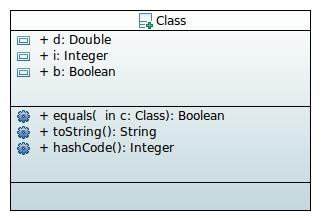
\includegraphics[width=0.4\textwidth]{uml/example.jpeg}
%	\caption{UML class diagram of questions representation.}
	\label{uml:example}
\end{figure}

%\begin{center}
%	\begin{tikzpicture}
%		\umlclass[y=-3]{Class}{
%			+ d : double \\ - i : int \\ \# b : boolean
%		}{ + equals(c : Class) : Boolean \\ + toString() : String \\ + hashCode() : Integer}
%	\end{tikzpicture}
%\end{center}

As we can see, the description of a class is divided into three sections, in the first there is its name, in the second its attributes and in the third its methods or behaviors. Attributes and methods can be either private $(-)$ to the class itself, protected $(\#)$ to the class and its children, or public $(+)$ to every other class.

In the example presented here there is a class named \textit{Class} with three attributes: a public attribute named $d$ of type \textit{Double}, a private attribute named $i$ of type \textit{Integer} and a protected attribute named $b$ of type \textit{Boolean}. Moreover, \textit{Class} has three methods:
\begin{itemize}[noitemsep]
	\item a method \textit{equals} which takes an element of the class \textit{Class} as input, compares it to the object on which this method is called and returns \textit{True} if they are the same objects, \textit{False} otherwise. The implementation of the method itself determine the meaning of similarity.
	\item a method \textit{toString} which does not take any input and returns the String corresponding to the current object. This value is often used for visualization purposes.
	\item a method \textit{hashCode} which does not take any input and produces an Integer value associated to the current object. This value is often used by the method \textit{equals} since same objects must return the same hash value. 
\end{itemize}

We described these three methods because they are basic methods that are automatically inherited by all classes. In fact, every class is an implicit child of a more general \textit{Object} class. If not specified these methods return the default mechanism that can lead to unexpected results. Although specified in our code, we decided to omit these methods from the uml diagrams as a matter of the clarity of the figure.

\subsection{Preference Representation}

\Cref{uml:preference} describes the basic elements of our elicitation software.
The two basic elements are represented by the \textit{Alternative} and \textit{Voter} objects. A \textit{Preference} is a list of alternatives in which the order represents the preference order. Multiple alternatives can have the same rank but an alternative cannot be associated to multiple ranks, i.e. it represents a linear order. Methods allow, for example, to know the alternative in a given rank or, conversely, to know the rank of a given alternative.
A \textit{StrictPreference} is an extension of the Preference object. This means that it inherits all of its behaviors and attributes but can redefine a given mechanism. In particular, StrictPreference does not allow two alternatives to have the same rank, i.e. it represents a strict order.
A \textit{VoterStrictPreference} links a Voter to her StrictPreference.
A \textit{PrefGraph} is a graph of preferences that can be added or modified. Specifically, each node represents an alternative, and an arc from a node $a$ to a node $b$ means that the alternative $a$ is preferred over the alternative $b$.
A \textit{VoterPartialPreference} links a Voter to her PrefGraph.

\begin{sidewaysfigure}
	\centering
	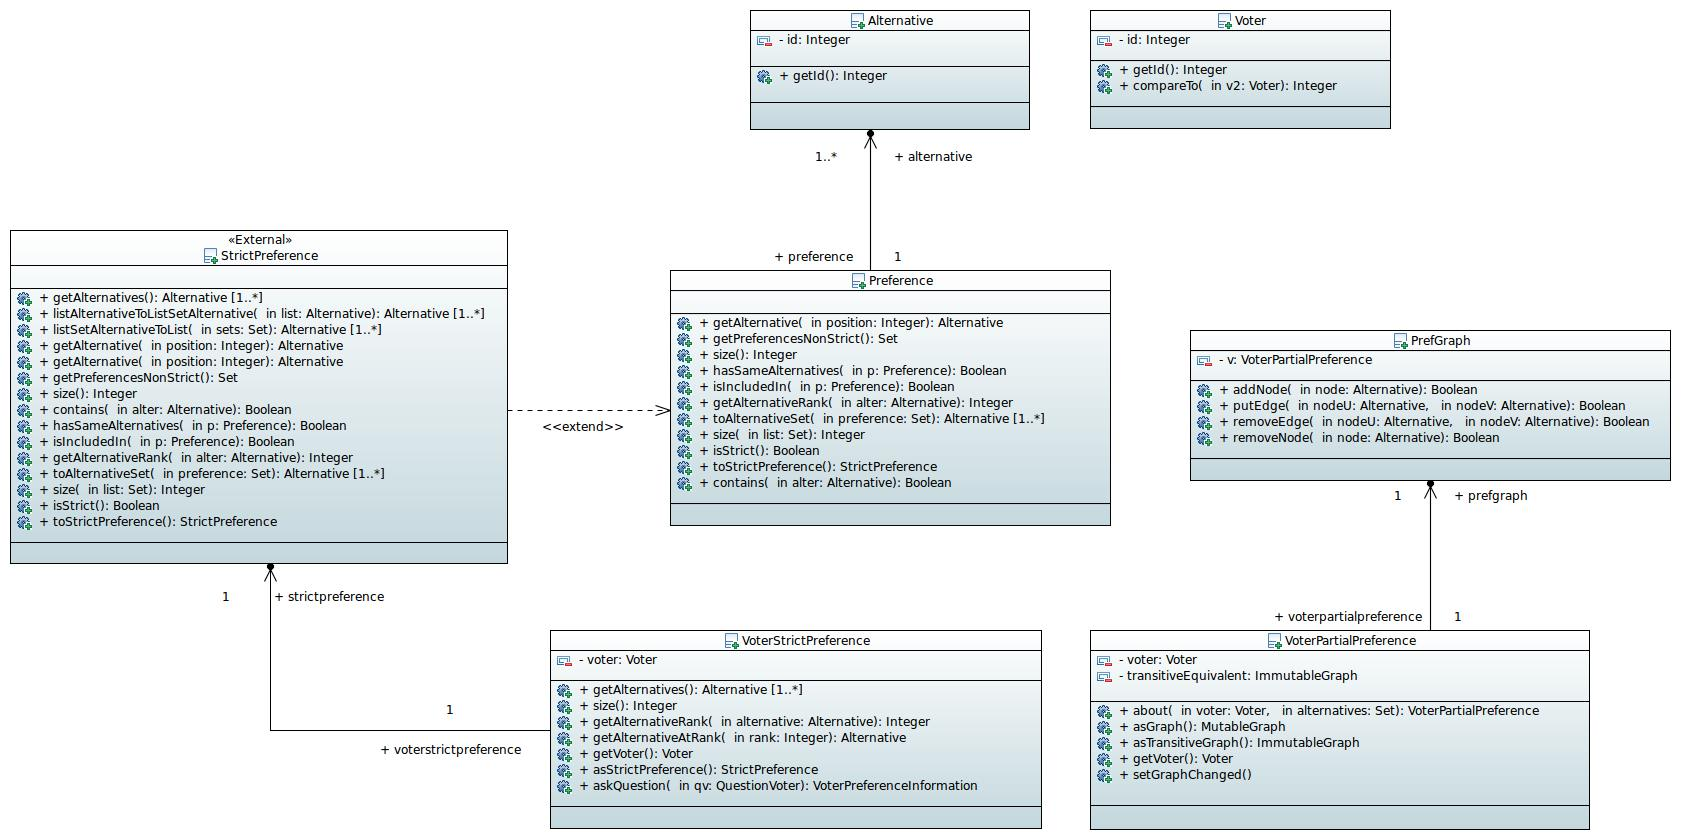
\includegraphics[width=\textwidth]{uml/basic.jpeg}
	\caption{UML class diagram of preferences representation.}
	\label{uml:preference}
\end{sidewaysfigure}

\subsection{Knowledge Representation}

\Cref{uml:knowledge} describes our approach to the representation of knowledge. We defined \textit{PreferenceKnowledge} as an interface, i.e. a completely abstract entity that define the structure that concrete objects must implement. An instance of PreferenceKnowledge must implements, among others, methods to return the alternatives, the voters, the profile and the constraints on the weights associated to rank positions.
A possible implementation is given by \textit{UpdateablePreferenceKnowledge} which keeps, as attributes, a partial profile and the constraints on weights and allows you to modify them. The \textit{ConstraintsOnWeights} are equations relating the difference between the weights of two consecutive pairs of ranks. It provides method to add constraints and to return an optimal set of weights that satisfies the constraints. Those weights are represented by \textit{PSRWeights} which is a list of rational numbers associated to the Positional Scoring Rule. Since in our framework we assume the convexity of weights the satisfaction of this condition is automatically checked when creating a new instance of this class.
Finally, in the diagram we can see an \textit{Oracle} class. This represents "true" knowledge, which exists but is unknown to us and which we try to elicit by asking questions. It contains the set of alternatives, the preferences of the chair\textemdash which are the weights of the scoring rule\textemdash and the preferences of the voters\textemdash which is the profile. During our elicitation procedure we ask questions to this entity.

\begin{sidewaysfigure}
	\centering
	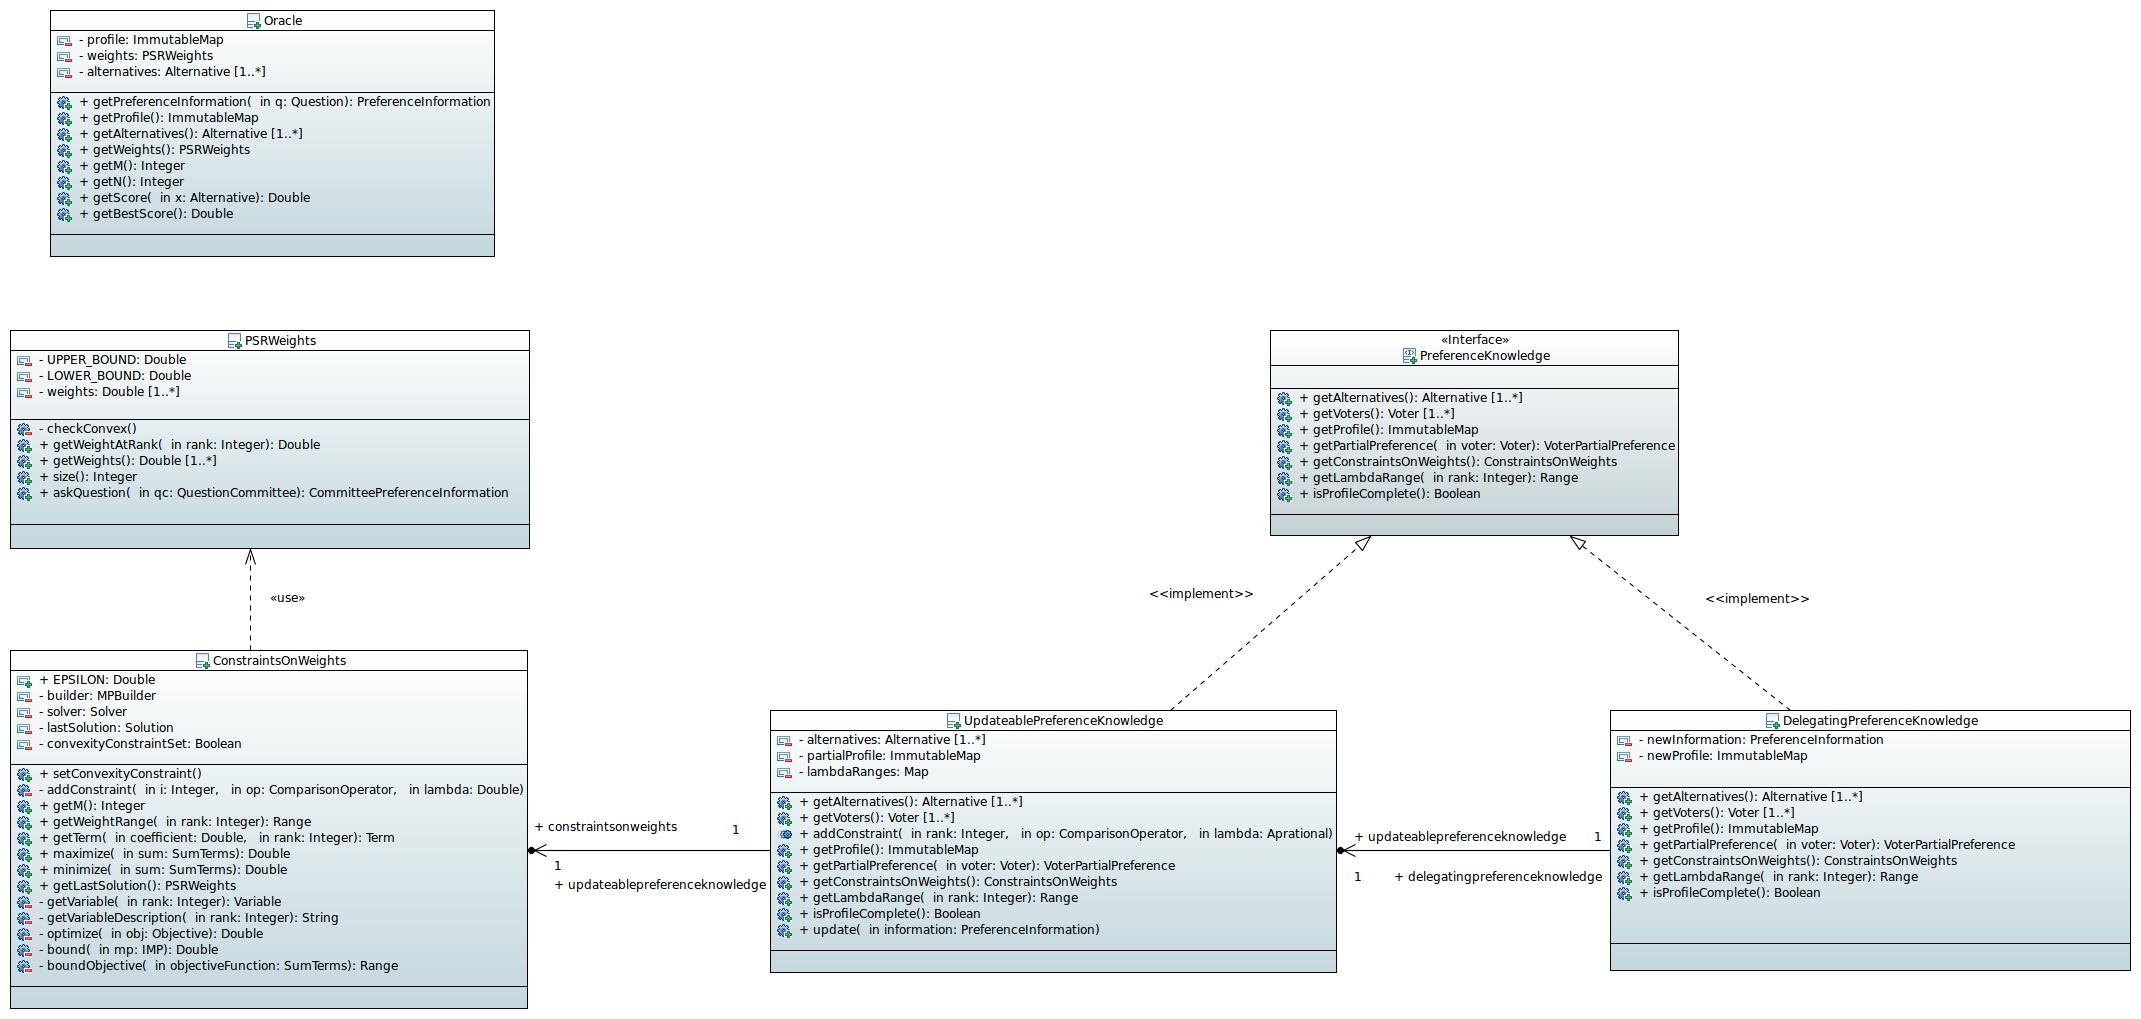
\includegraphics[width=\textwidth]{uml/knowledge.jpeg}
	\caption{UML class diagram of knowledge representation.}
	\label{uml:knowledge}
\end{sidewaysfigure}

\subsection{Questions Representation}

\Cref{uml:questions} shows the diagram related to the questions implementation. A \textit{Question} can be either a question to the chair, about their preferences on the voting rule, or a question to one of the voters, about their preferences over the alternatives. This is represented by the use of an enumeration \textit{QuestionType} that admits only two values: VOTER$\_$QUESTION and COMMITTEE$\_\allowbreak$QUESTION.
The method \textit{getType()} of \textit{Question} returns one of those two values.
A \textit{QuestionVoter} is a comparison query relating two alternatives $a$ and $b$, where \textit{getPositiveInformation()} returns the \textit{VoterPreferenceInformation} (see \Cref{uml:prefinfo}) associated to that specific voter and the alternative $a$ and $b$. Conversely, \textit{getNegativeInformation()} returns the information regarding the alternative $b$ and $a$. In other words, the first method returns the information when the answer to the question "$a\pref b ?$" is yes, thus $a$ is preferred to $b$, and the second method that when the answer is no, thus $b\pref a$.
A \textit{QuestionCommittee} tries to improve the knowledge about the scoring rule by refining the multiplier $\lambda$ in the constraint $w_{r} - w_{r+1} \geq \lambda (w_{r+1} - w_{r+2})$ for some $r \in \{1,\ldots,m-2\}$. Given a $\lambda$ and a rank defined by an elicitation strategy, \textit{getPositiveInformation()} returns the response to the following question "$w_{r} - w_{r+1} \geq \lambda (w_{r+1} - w_{r+2})?$". The complementary method, \textit{getNegativeInformation()}, returns the information of the opposite question $"w_{r} - w_{r+1} \leq \lambda (w_{r+1} - w_{r+2})?"$.
Positive and negative information is used by the elicitation strategies for the choice of the next question to ask. In particular, the Pessimistic strategy considers, for each potential question, the information in case of positive and negative answer and picks the question that leads to minimal regret in the worst case. This is described in \Cref{uml:strategies}, in particular in the class diagram of \textit{MmrLottery}.


\begin{figure}
	\centering
	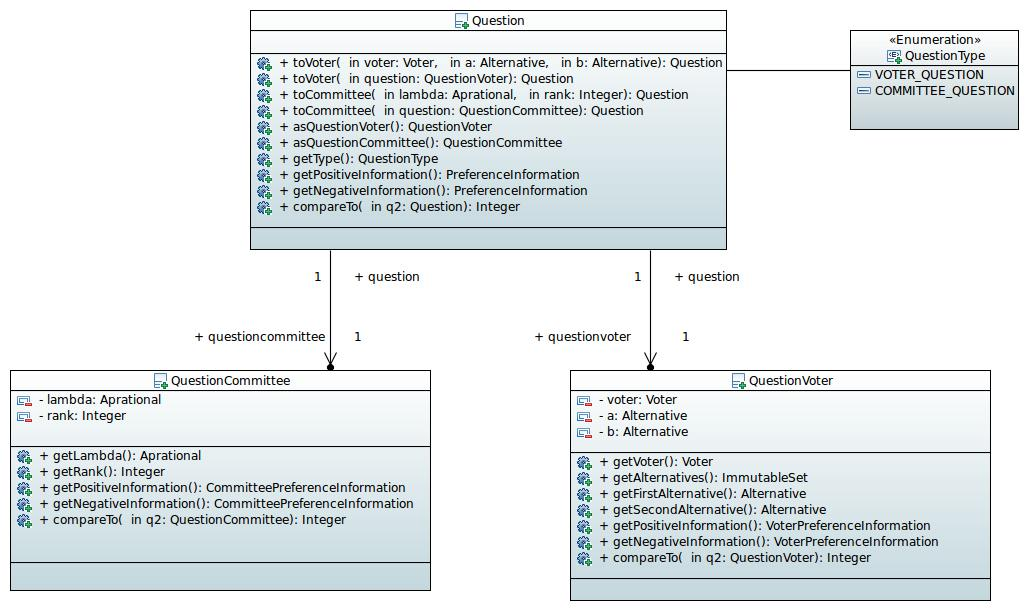
\includegraphics[width=\textwidth]{uml/questions.jpeg}
	\caption{UML class diagram of questions representation.}
	\label{uml:questions}
\end{figure}

\subsection{Preference Information}

\Cref{uml:prefinfo} illustrates the diagram related to the information about preferences acquired by asking questions. With a similar representation to the questions themselves, \textit{PreferenceInformation} can be of two types: \textit{CommitteePreferenceInformation} or \textit{VoterPreferenceInformation}. The type of the information depends on the type of the question asked.

\begin{figure}
	\centering
	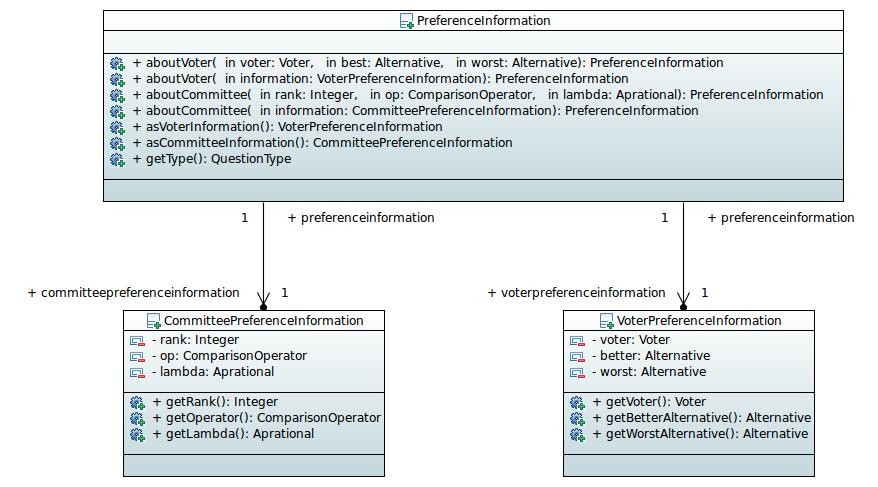
\includegraphics[width=\textwidth]{uml/prefinfo.jpeg}
	\caption{UML class diagram of elicited knowledge obtained by asking questions.}
	\label{uml:prefinfo}
\end{figure}

\pagebreak

\subsection{Regret Computation}
\Cref{uml:regret} is the diagram representing the procedure described in \Cref{sec:mmr}. The \textit{PairwiseMaxRegret} is the building block of the regret computation. Given two alternatives, their ranks and the weights associated to ranks, it computes the regret of choosing the first alternative instead of the second one. This is used by the \textit{Regrets} instance, which calculate the minimal max regret value and it can return all the alternatives associated to such value. A small constant epsilon is introduced to express the granularity of this similarity. In fact, we may want to consider two weights equals if, for example, they are equal up to the third decimal place. \textit{RegretComputer} is the class that handles the proper calling of the methods specified by the classes aforementioned. For example by providing the pairwise maximum regret computation with the worst-case scenario: the worst completion of profile and scoring vector.


\begin{figure}
	\centering
	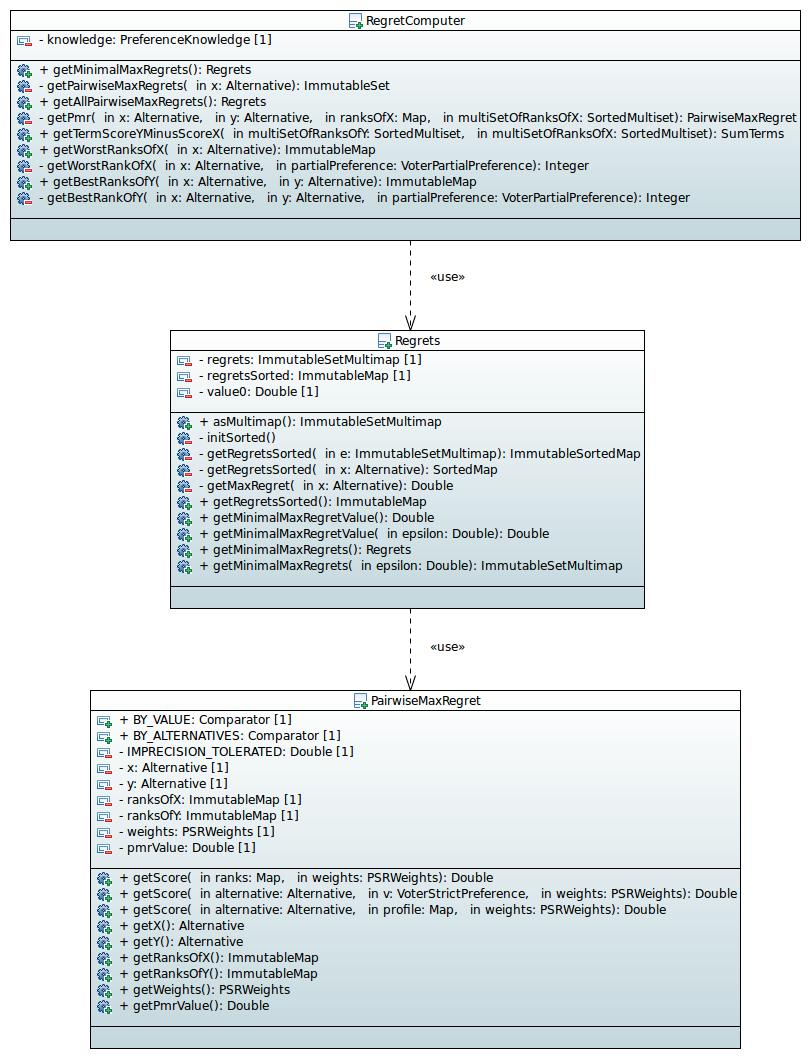
\includegraphics[width=\textwidth]{uml/regret.jpeg}
	\caption{UML class diagram of regret computation.}
	\label{uml:regret}
\end{figure}


\subsection{Strategies}

\Cref{uml:strategies} describe our design of elicitation strategies. A \textit{Strategy} is an interface that specify two methods: \textit{setKnowledge} that sets and updates the knowledge collected so far, and \textit{nextQuestion} that returns the next question to ask. Every strategy, i.e. every implementation of \textit{Strategy}, must define those two methods. We created an enumeration for the \textit{StrategyType} based on the different strategies we implemented and tested.
In particular, the ones discussed in \Cref{sec:elicit} are \textit{StrategyByMmr} that, depending on the parameters with which it is invoked, corresponds to \textit{Pessimistic}, \textit{Extended pessimistic} or \textit{Two Phases}, \textit{StrategyElitist} that corresponds to \textit{Elitist} and \textit{StrategyRandom} that corresponds to \textit{Random}.
Please see \Cref{sec:elicit} for a detailed explanation of their behaviors and performances.
From a design point of view, each strategy defines the interface methods and it makes use of a \textit{StrategyHelper} for all those functions common to each strategy. For example, to get all the pairs of alternatives whose order is already known and therefore it does not make sense to ask about; or to find the voters to whom we can still ask questions and, eventually,all those possible questions.
Finally, \textit{StrategyFactory} is an object that handles the creation of the desired strategy without disclosing to the user the strategy's creation logic.

The java package containing all those classes and also the UML diagrams can be found at \url{https://github.com/oliviercailloux/minimax}.

\begin{sidewaysfigure}
	\centering
	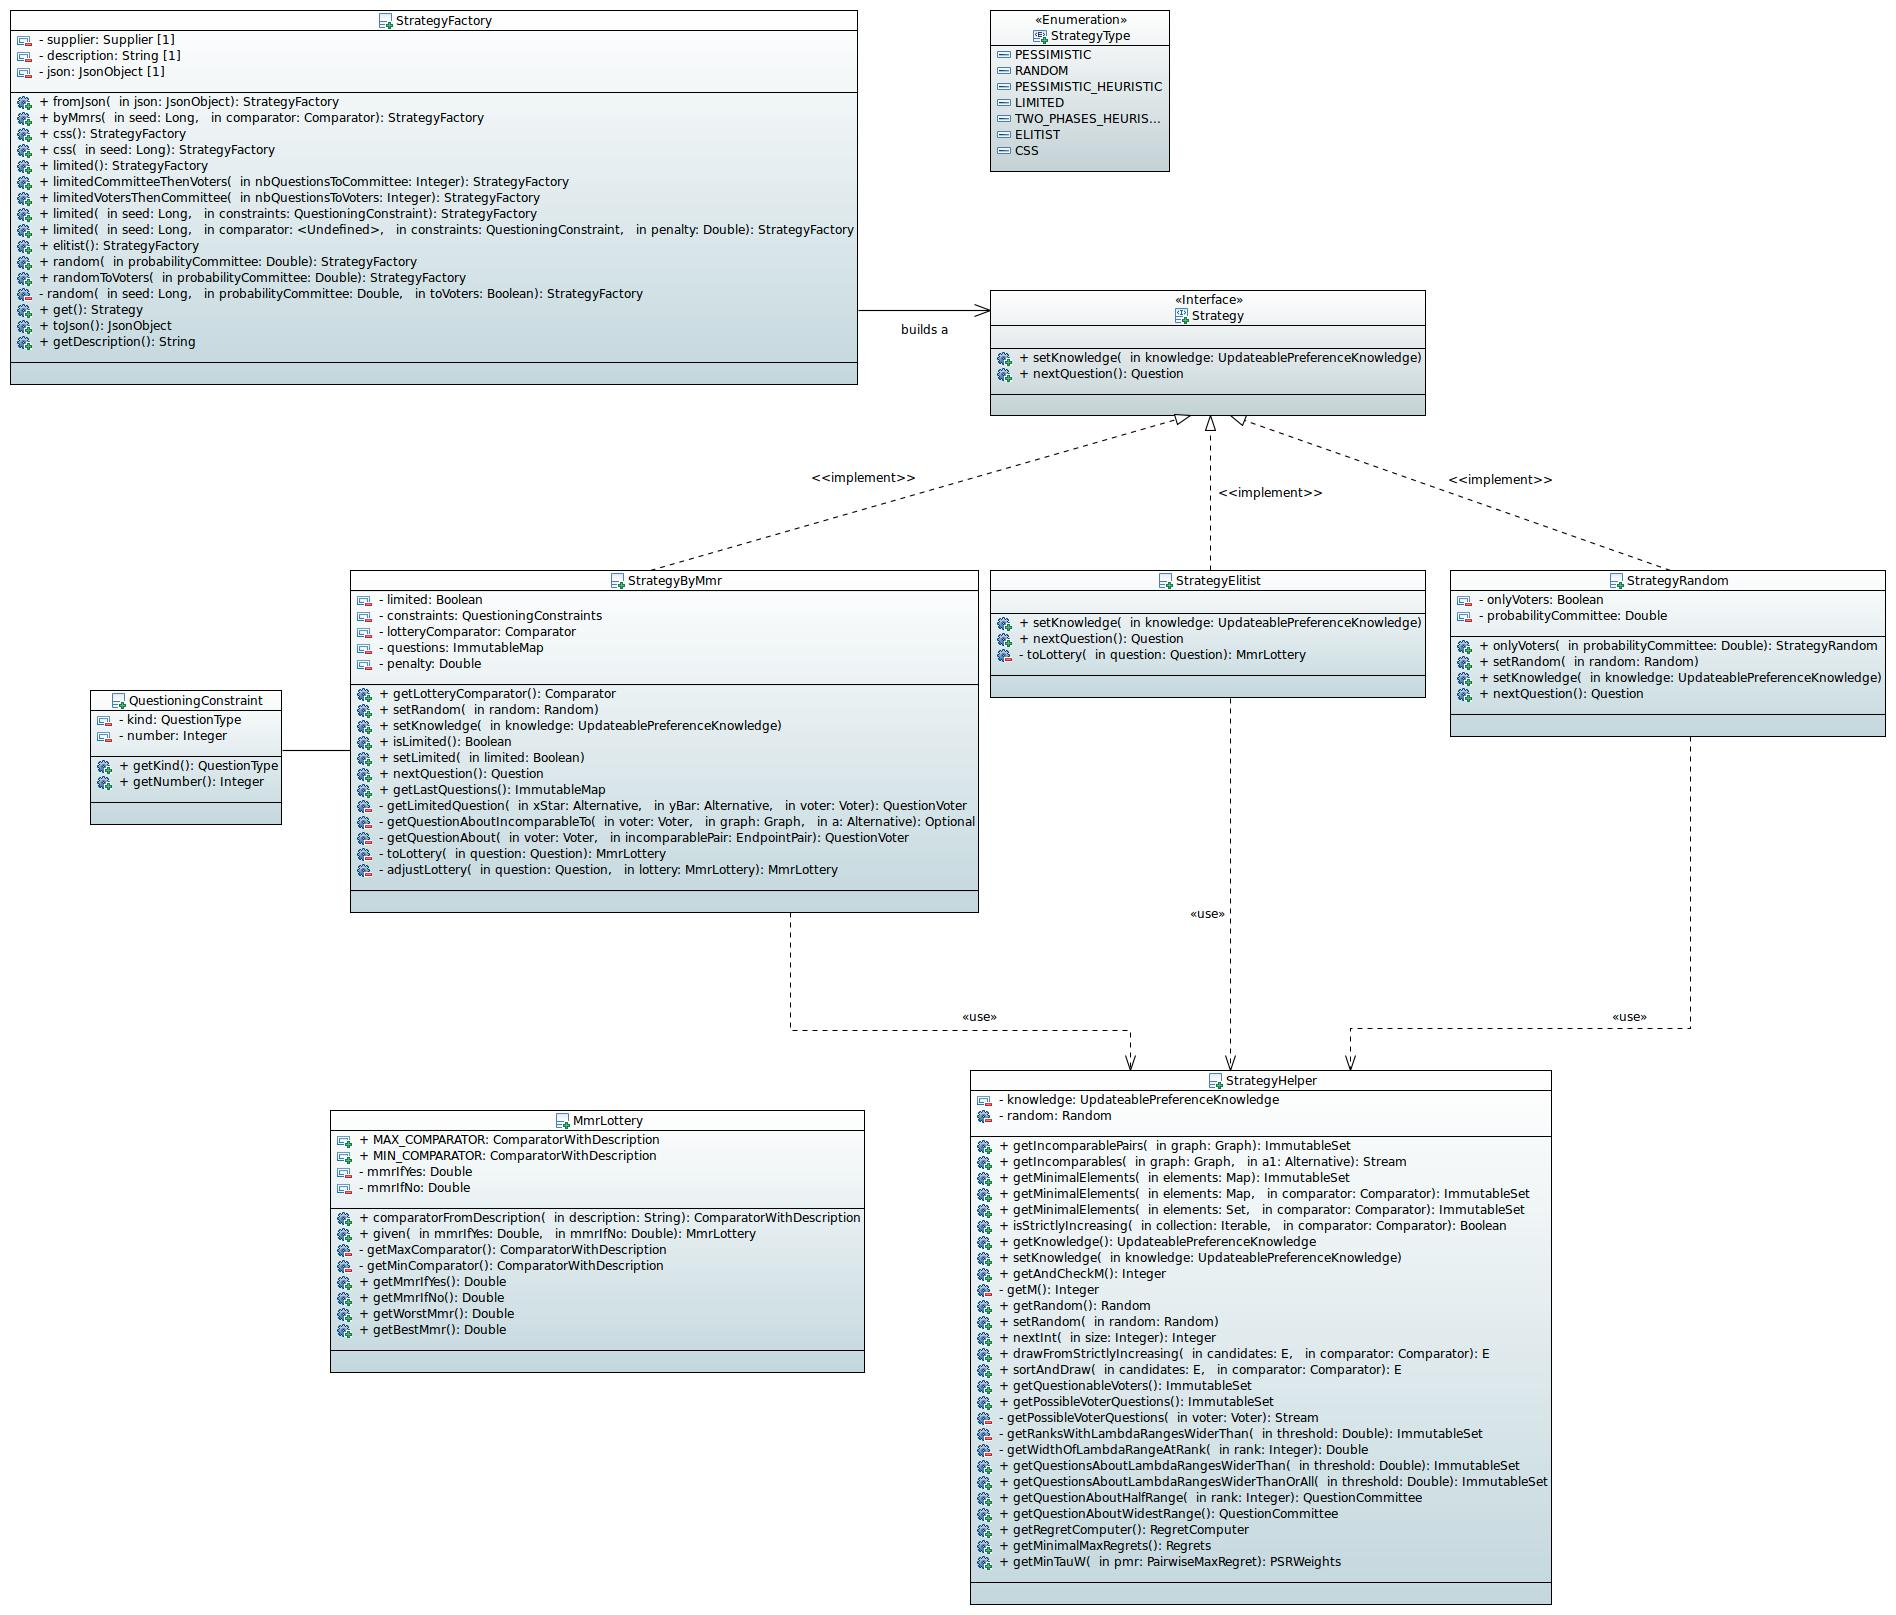
\includegraphics[width=0.8\textwidth]{uml/strategies.jpeg}
	\caption{UML class diagram of strategies.}
	\label{uml:strategies}
\end{sidewaysfigure}

	\chapter{Majority Judgment winner determination under incomplete information}
		\label{ch:MJ}
		%!TeX root= ../thesis.tex

\begin{abstract}
\ac{MJ} is a voting system where voters assign grades to candidates using an ordinal scale. The winner is the candidate with the highest majority-grade \textemdash which is the median of the grades received. This method has attracted increasing attention of french associations and political parties which have started to use \ac{MJ} for internal decisions or local elections. In particular LaPrimaire.org is a french association that uses \ac{MJ} to choose its candidate for the french presidential election. The vote is conducted in two rounds: in the first one the voters judge five candidates randomly picked; the five candidates with the highest medians pass at the second round as finalists and the voters are asked to judge them. Is the random selection of candidates a good elicitation technique? In this paper we explore the consequences of profile incompleteness and prove that this method can fail to elect the winning candidate of the complete profile. Furthermore, we perform experiments on randomly generated profiles and profiles following the grade distribution of a real voting scenario. We find that the probability of not selecting the winner of the full profile greatly decreases as the number of voters increases and we investigate how much of the grade vector we should know in order for this probability to be low. 
\end{abstract}

\section{Introduction}
\label{sec:intro}
\ac{MJ} is a voting method proposed by \citet{Balinski2007,Balinski2011} to elect one out of $m$ candidates based on the judgments of $n$ voters. The latter express their preferences by assigning to each candidate one of the following adjectives: Excellent, Very good, Good, Average, Mediocre, Inadequate, To be rejected. Those adjectives represent a common language whose semantic is assumed to be a shared knowledge among the voters carrying thus an absolute meaning. For each candidate the median of the grades she received is computed, this is called \textit{majority-grade}. The candidate with the highest majority-grade is elected. Ties are broken by considering the majority-grade of first order: one vote associated with the majority-grade of each tied candidates is removed and their medians are recomputed. The candidate with the highest new median is elected. If there is still a tie the process is repeated until a unique winner is found. 

In the last few years \ac{MJ} has being adopted by a progressively larger number of french political parties including: Le Parti Pirate, Génération(s), LaPrimaire.org, France Insoumise and La République en Marche.
%https://www.lopinion.fr/edition/politique/en-marche-teste-elections-jugement-majoritaire-mode-scrutin-tres-201884
"Mieux Voter" \citep{MV} is a french association that promotes the use of \ac{MJ} as voting method whenever a collective choice has to be selected: public administration, associations, companies. On their website it is possible to find all the citizens lists \textendash party lists that are not affiliated to any national political party \textemdash that used \ac{MJ} to rank their candidates during the local elections of 2020. In two cases, Bordeaux et Annecy, the candidate selected using \ac{MJ} was then elected as a mayor. 

In particular, LaPrimaire.org \citep{LaPrimaire} is a french political initiative whose goal is to select an independent candidate for the french presidential election using \ac{MJ} as voting rule. The association Democratech implemented the platform for the first time in 2016 in view of the 2017 presidential elections. The number of voters who participated in the election was $10676$ during the first round, and $32685$ during the second round.

The procedure that they adopted consists of two rounds. In the first round each voter is asked to express her judgment, using \ac{MJ}, on five random candidates. At the end of this phase the five candidates with the highest medians are considered the finalists who qualify for the second round. In the second round each voter is asked to express her judgment, using \ac{MJ}, on all the five finalists. The candidate with the best median at the end of this phase is selected as representative for the presidential election.

In this paper we analyze this elicitation process of voters preferences. In particular, we investigate the consequences of randomness when asking the voters to judge candidates. We evaluate the cost of this procedure \textemdash which can be quantified as number of questions per voter \textemdash and its fairness for candidates \textemdash which reflects the idea that a potential winner should not loose for lack of information.


\subsection{Related work}

One of the earliest uses of the median as an aggregator in voting theory can be identified in the \textit{middlemost} method proposed by \citet{Galton1907a,Galton1907b}. In particular, in situations where a group of people had to assess a damage, he suggested the median as the only method that does not suffer from over- or under-exaggerations.

We can consider the median grade as the highest level at which a candidate obtains the support of the majority of the voters. Starting for the highest grade $\delta$ we check if the majority of the voters assigned at least $\delta$ to some alternative. If this is not the case, we descend in the grading scale until such level $\delta^*$ is found. The grade $\delta^*$ is the median of grades associated to some alternative, and, since it is the first level we stopped at, it corresponds to the best possible median. This method was rediscovered several times and proposed under the name of Bucklin's rule \citep{Hoag1926}, Majoritarian Compromise \citep{Sertel1986,Sertel1999} and q-approval fallback bargaining \citep{Brams2001}. Moreover, when the number of grades is equal to two (approve, disapprove) then it is reduced to Approval Voting.

More recently \citet{Bassett1999} proposed the use of the median as voting rule for elections advocating for its robustness.
Several studies on the use of the median have been conducted. In particular, \citet{Bassett1994} and \citet{Gehrlein2003} study its manipulation. \citet{Barthelemy1981} survey mathematical problems and properties related to the notion of median in the context of cluster analysis and social choice theory. \cite{Nehring2022} analyze the median rule in judgment aggregation and they define a weighted median rule that is equivalent to \acs{MJ} except for the treatment of ties.

However, there is a significant concern that has never been analyzed when considering \ac{MJ}. Asking voters to provide a grade for each of the candidates can have a high cognitive and communicative cost. In situations where the set of alternatives is very large, voters may not be able to assign a significant and informed grades. \citet{Conitzer2005} studied the complexity of communication of some of the most common voting rules.
In these cases, elicitation strategies exist to retrieve the most relevant information. \citet{Konczak05} introduced the notion of possible and necessary winners. This paved the way for procedures that attempted to find necessary winners by asking voters the fewest questions possible \citep{Kalech2011}.
Considering scoring rules, \citet{Lu2011} suggested the use of minimax regret as a guide to the elicitation procedure. \citet{Bachrach2010} proposed a probabilistic approach. Several authors studied the complexity of determining when to stop the elicitation process for some of the most common voting rules \citep{Conitzer2002, Walsh2009}.
However, to the best of our knowledge, there are no works on preferences elicitation considering \ac{MJ}.

Very recently, \citet{Varloot2022} considered a version of \ac{MJ} under uncertainties in order to study its strategyproof properties. Their premise, however, is based on the fact that voters who are uncertain about the degree to assign to an alternative would instead assign to it a probability distribution. In other words, if a voter does not know whether to assign good or excellent to a certain alternative, then she may assign to it, for example, good with $\frac{1}{3}$ of the probability and excellent with $\frac{2}{3}$ of the probability. 
This approach requires the submission of even more information and is very far from our idea of incomplete knowledge.


\section{Notation}
\label{sec:complete}
Consider a finite set $N=\{i_1, \dots, i_n\}$ of voters (or judges) and a finite set $A=\{j_1, \dots, j_m\}$ of alternatives (or competitors). 
A \textit{common language} $\triangle = \{ \delta_1, \delta_2, \dots \}$ is a set of strictly ordered grades, and the notation $\delta_1 \geq \delta_2$ indicates that $\delta_1$ is a better or equivalent grade than $\delta_2$. A profile $P : A\times N \rightarrow \triangle$ is a $m$ by $n$ matrix of grades. Given any $N'\subseteq N$, the operator $\rho: \triangle^{N'} \rightarrow \triangle^{\card{N'}}$ defines an ordering function that given a vector of grades $P_j$ returns the vector ordered by decreasing grades.

Consider a set of alternatives $S\subseteq A$,
%where $|S|=s$ and $s \in \intvl{1,m}$ \textemdash the double brackets represent an interval in the integers. 
we denote by $P^S \in \triangle^{S \times N}$ a restriction of the profile $P$ to only the alternatives in $S$, $P^S \subseteq P$. Note that when $S=A$ then $P^S=P$.
%\commentOC{Could also write $\restr{P}{S × N}$, which leads to more generality, if restricting the users is also sometimes convenient.}

%We let $f: \triangle^{N} \rightarrow \triangle$ denote a function that assigns to any vector of grades a final grade. Given any $S\subseteq A$, a grading function $f^S: \triangle^{S \times N} \rightarrow \triangle^S$ returns a vector of final grades by applying $f$ to every alternative in $S$.
% the \emph{middlemost} aggregation function $f$, for each vector of grades $r_i= (r_1 , \dots, r_n )$ associated to the alternative $i \in \intvl{1,m}$, returns: 
%\begin{align}
%	f(r_i) &= r_{(n+1)/2} \text{ when n is odd,} \\
%	r_{n/2} \geq f(r_i) &\geq r_{(n+2)/2} \text{ otherwise.}
%\end{align}

We let $\fmaj:\triangle^{N} \rightarrow \triangle$, denote the \emph{majority-grade} function that associates to a vector of grades $\emptyset \neq v \in \triangle^{N'}, N' \subseteq N$ its median grade value: $\fmaj(v) = \rho(v)_{\floor{\frac{\card{v}}{2}} + 1}$. Note that in case $\card{v}$ is even, two medians could be used, but, as in \citet{Balinski2011} definition, the lower grade is picked. 

%Given any $S\subseteq A$, by applying $\fmaj$ to all vectors of grades associated to the alternatives in $S$ we obtain the corresponding grading function $\fmaj[S]$. Formally, $\fmaj[S](P^S)_j = \fmaj[S](P^S_j)$. The $j$-\emph{th} element of the resulting vector is the median of the ordered vector of grades associated to the $j$-\emph{th} alternative. 
%%Because $f^S_{maj}(P^S)_i$ depends only on $P^S_i$ we write $f^S_{maj}(P^S_i)$. \commentOC{I am not sure I follow. You already have a notation for this, namely, $\fmaj(P^S_i)$, isn’t it?}
%Moreover, when we consider the complete profile (when $S=A$) we will write $\fmaj(P_j)$ instead of $\fmaj[A](P^A_j)$.
%\commentOC{I doubt that the general $f$ is actually useful, you only seem to use $f$ maj.}
%\commentOC{The argument doesn’t seem correct to me, in $\fmaj[A](P^A_j)$.}
%\commentOC{I find it confusing to use the same symbol ($\fmaj$) for two quite related but distinct functions.}
%i.e. it corresponds to the lower middlemost.

Given any $S\subseteq A$, the winner function $\Fmaj[S]:\triangle^{S \times N} \rightarrow A$ %$F^S_{maj}:\triangle^{S \times N} \rightarrow 2^A \setminus \emptyset$
is a function that given $|S|$ alternatives and their median grade, selects the alternative with the highest median grade as winner. We can define it as  $\Fmaj[S](P^S) = \argmax_{j\in S}\fmaj(P^S_j)$ assuming it is a singleton. 
For brevity, we will write $\Fmaj$ when considering $S=A$.
To avoid adding further complexity to the notation, we describe only informally what happens in case multiple alternatives are tied for the highest median grade $h$, thus, when $\argmax_{j\in S}\fmaj(P^S_j)$ is not a singleton.
In this case, ties are broken by removing one $h$ grade from the vectors of grades of each tied alternative, recomputing the new median grade and repeating the process until one unique winner is found or there are no more grades to remove. When $n$ is odd, this is equivalent to take the next element after the median, i.e. the one at index $(\floor{\frac{n}{2}} + 1) +1$. If there is still a tie we then look at the previous element before the median, i.e. the one at index $(\floor{\frac{n}{2}} + 1) -1$, and keep alternating until the tie is broken or there are no more elements in the vector. When $n$ is even the element before the median, i.e. the one at index $\floor{\frac{n}{2}}$, is taken first and, if there is still a tie, then the element after the median is considered, i.e. the one at index $\floor{\frac{n}{2}} + 2$, and so on. If after applying the mechanism there are still ties we break them using an arbitrary ordering defined on all alternatives, e.g. lexicographical order.

Similarly to the winner function, given any $x \in \intvl{1,m}$, we can define a more general \emph{selection function} $F^S_x:\triangle^{S\times N} \rightarrow \powersetz{A}$, where $\powersetz{A}$ is the powerset of $A$ excluding the empty set, that selects exactly the $x$ alternatives with the $x$ highest median grades. Thus, $F^S_x(P^S) = \Fmaj[S](P^S) \cup \Fmaj[S'](P^{S'}) \cup \dots \cup \Fmaj[S^{k-1}](P^{S^{k-1}})$ where $S'= S \setminus \Fmaj[S](P^{S})$, $S''= S \setminus \Fmaj[S](P^S) \setminus \Fmaj[S'](P^{S'})$ etc.


\subsection{Incomplete knowledge}
In order to analyze the elicitation procedure used by LaPrimaire.org, we need to adapt the notation just described to incomplete profiles. 
Let $\Pbar$ be our knowledge about the profile $P$.
The voters have full knowledge of their own judgments but we ignore them; our goal is to elicit them by questioning the voters starting from zero knowledge.
We introduce an additional grade $\dbar$, and, given a language $\Delta$, $\dbar< \delta, \forall \delta \in \Delta$.
%\commentBN{I think we should avoid to say this but rather add in $\bar{F}$ that the $\dbar$ are excluded.}
The common language in the incomplete knowledge setting is then $\overline{\triangle}=\triangle \cup \dbar$. Voters cannot use this grade to express their judgment over an alternative and it does not count in the computation of the median grade as we will explain formally. We refer to the grades in $\triangle$, the ones used by voters, as "defined" grades.

Let $\Pbar\in \overline{\triangle}^{A \times N}$ denote an \emph{incomplete profile}, i.e. a matrix $m \times n$ of grades some of which are "undefined".
The starting knowledge is represented by a matrix $m\times n$ of $\dbar$ grades. Given $k \in \N$, we define with $K_i \subseteq A$ a set of $k$ alternatives that we ask the voter $i\in N$ to evaluate. 
After having asked every voter in $N$ to judge $k$ candidates, we obtain an incomplete profile $\Pbar^k$, that is a matrix $m \times n$ of grades of which $kn$ are "defined".
Note that when $k=m$, the resulting profile $\Pbar^k$ corresponds to the complete profile $P$. Let $C(\Pbar)$ be the set of all completions of $\Pbar$ obtained by substituting all $\dbar$ grades with "defined" ones, note that $P \in C(\Pbar)$.
%if we want to define $C(\Pbar) = \{P' \in \triangle^{m \times n} \suchthat \restr{\Pbar}{\triangle} \subseteq P'\}$ then we introduce $\restr{\Pbar}{\triangle} = \Pbar \cap (A \times N \times \triangle)$
 
%If $K_i=K_l, \forall i,l\in N$, i.e. if we ask all voters to judge the same $k$ alternatives, then we have complete knowledge restricted to this set of candidates. We denote with $P^{K_i}$ the restriction of the complete profile $P$ to only the alternatives in $K_i$.
%\commentOC{I wonder if this notation will be useful.}

Let $g:\overline{\triangle}^N\rightarrow \bigcup_{N' \subseteq N}\triangle^{N'}$ be the function that given an incomplete vector of grades $q \in \overline{\triangle}^N$, thus $q \subseteq N × \bar{\triangle}$, returns the vector composed only of the "defined" grades. 
%$g(q) = \restr{q}{N × \triangle}$ \commentOC{This should be $q \cap (N × \triangle)$, but anyway as above this may be more complexity that what we do with this afterwards justifies, so perhaps omitting what $g$ is formally (especially considering that this union is not straightforward to understand) may be beneficial to the reader.}.

%The operator $\overline{\rho}$ defines a restricting ordering function that given $\overline{P_i}$, an incomplete vector of $n$ grades, returns the correspondent complete vector restricted to its $x$ "defined" grades decreasingly ordered: $\overline{\rho}(\overline{P_i})=\rho(d(\overline{P_i}))$. \commentBN{Not sure this is necessary.}

The \emph{majority-grade} for incomplete profile $\fmajbar: \overline{\triangle}^N \rightarrow \triangle$ corresponds to $\fmaj$ that only considers the "defined" grades in the computation of the median. Consider an incomplete grade vector $\overline{P}_j$ and let $P'_j=g(\Pbar_j)$ be the partial vector of $\overline{P}_j$ of only "defined" grades, then \[\fmajbar(\Pbar_j)= \left\{ \begin{array}{cl}
	\fmaj(P'_j) =  \rho(P'_j)_{\floor{\frac{\card{P'_j}}{2}} + 1} & \mbox{for } \
	 P'_j \neq \emptyset  \\  \dbar & \mbox{otherwise}
\end{array}\right.
\]
In a similar fashion, we can define $\Fmajbar[S](\Pbar)=\argmax_{j\in S}\fmajbar(\Pbar^S_j)$ and, given a value $x\in \intvl{1,m}$, the selection function of the $x$ best alternatives is $\overline{F}^S_x(\Pbar^S) = \Fmajbar[S](\Pbar^S) \cup \Fmajbar[S'](\Pbar^{S'}) \cup \dots \cup \Fmajbar[S^{x-1}](\Pbar^{S^{x-1}})$ where $S'= S \setminus \Fmajbar[S](\Pbar^{S})$, $S''= S \setminus \Fmajbar[S](\Pbar^S) \setminus \Fmajbar[S'](\Pbar^{S'})$ etc.

To summarize the elicitation process we want to investigate, starting with zero knowledge, each voter is asked to evaluate $k$ candidates. Given the partial information at our disposal, we are able to define the "known" median grade for each alternative by applying $\fmajbar(\Pbar^k_{j}), \forall j\in A$. We can then use the \emph{selection function} $\overline{F}_k$ to select the $k$ alternatives with the highest "known" median grades. We denote this set of alternatives with $K=\overline{F}_k\subseteq A$. The alternatives in $K$ will be presented to all voters, who must provide a grade for each of them, thus obtaining a restriction of the complete profile to this subset of $k$ alternatives. From here, we can use $\Fmaj[K](P^K)$ to select the winning alternative of the restricted profile $P^K$.

%I'm not sure the following is relevant
%
%Given the set $\tilde{K}=F^S_k(g(\Pbar^S_j))$ of the best $k$ alternatives, every voter is then asked to judge all the candidates in $\tilde{K}$. 
%\commentOC{$i$ is not defined; and there may be a type incompatibility between the result of $g$ and the domain of $F^S_k$.}
%
%This process results in a restriction $P^{\tilde{K}}$ of the complete profile $P$. It is important to mention that when we ask the voters to judge an alternative $i\in \tilde{K}$ we assume that they report their preference as they would have stated it when asked about $P$. In other words, $P^{\tilde{K}}_{i} = P_j$ for any $i \in \tilde{K}$.
%\commentOC{The formal part of this does not look like your informal hypothesis.}
%
%Please note that $P^{\tilde{K}}$ is a complete matrix of $kn$ grades and that we fall back to the complete profile case, thus, we apply the \emph{majority-grade}, $\fmaj[\tilde{K}]$, function to $P^{\tilde{K}}$ to determine the median grades and then the winner function $\Fmaj[\tilde{K}]$ to select the winner. 
%For simplicity we denote by $\overline{W}_{\overline{P^k}} \subseteq A$ the results of this process.

\begin{remark}
	Because we are interested into investigating \acs{MJ}, we are going to use an alphabet with the same size of the one proposed by \citet{Balinski2011} which is composed of the following adjectives: To be Rejected, Inadequate, Mediocre, Average, Good, Very Good, Excellent. For brevity we are gonna rename those adjectives respectively from $\delta_1$, corresponding to To be Rejected, to $\delta_7$, corresponding to Excellent. Therefore, $\triangle=\{\delta_1,\delta_2, \delta_3,\delta_4,\delta_5,\delta_6,\delta_7\}$ 
\end{remark}

\section{Reasoning on incompleteness}
Let us now consider the effects of incomplete knowledge on the selection of a winner. In particular, we want to prove that if we consider an incomplete profile and take the $k$ alternatives with the highest median grade, with any $k$ being between $1$ and $m-1$, it is possible to miss the winner of one of its completion. 
This is important because in the elicitation process implemented by LaPrimaire.org, only the full grade vectors of the $k$ alternatives with the highest median grade are considered. Clearly, if the winning alternative in the complete profile is in this set $K \subset A$, then she will also be the winner of the incomplete profile. This is because the voters will be asked to provide a grade for all those $k$ alternatives, providing thus a restriction of the complete profile to only the alternatives in $K$. If a candidate is a winner for a complete profile, then she is also a winner for any of its restrictions that include her.
Note that this is not true in case of multiple winners where ties that cannot be broken by tie-breaking procedures and for which arbitrary ordering is, therefore, necessary. In what follows we assume the absence of such ties.
We want to show that it is possible for the winning alternative of the complete profile not to be included in this subset $K$ of alternatives.

	\begin{theorem}
		\label{th:notinK}
		Given a set $A$ of alternatives $m\geq 2$, a set of voters $N$ and a value $k\in \intvl{1,m-1}$, there exist a complete profile $P$ and an incomplete profile $\Pbar$ such that $P \in C(\Pbar)$ and $\Fmaj(P) \nsubseteq \overline{F}_k(\Pbar)$.
	\end{theorem}
	\begin{proof}
		Consider the following complete profile $P$
		\begin{center}
			$
			\begin{array}{ccccc}
				& i_1 & i_2 & \dots & i_n \\
				j_1 &	\delta_7 & \delta_7 & \dots & \delta_7 \\
				j_2 &	\delta_6 & \delta_6 & \dots & \delta_6 \\
				. &	\delta_6 & \delta_6 & \dots & \delta_6 \\
				j_m &	\delta_6 & \delta_6 & \dots & \delta_6 \\
			\end{array} \quad,
			$
		\end{center}
		where all voters judge all alternatives $\delta_6$ except for the alternative $j_1$ which is judged $\delta_7$ by everyone.
		The median grade of the alternative $j_1$ is $\fmaj(P_{j_1})=\delta_7$ and the one of all the other alternatives is $\fmaj(P_x)=\delta_6, \forall x \in A \setminus \{j_1\}$. Thus, the winner in the profile $P$ is $\Fmaj(P)=\{j_1\}$.
		Consider now the following incomplete profile $\Pbar$:
		\begin{center}
			$
			\begin{array}{ccccc}
				& i_1 & i_2 & \dots & i_n \\
				j_1 & \dbar & \dbar & \dots & \dbar \\
				j_2 &	\delta_6 & \delta_6 & \dots & \delta_6 \\
				. &	\delta_6 & \delta_6 & \dots & \delta_6 \\
				j_m &	\delta_6 & \delta_6 & \dots & \delta_6 \\
			\end{array} \quad.
			$
		\end{center}
		The median grade of $j_1$ under the profile $\Pbar$ is $\fmaj(\Pbar_{j_1})=\dbar$ and the one of all the other alternatives is $\fmaj(\Pbar_x)=\delta_6, \forall x \in A \setminus \{j_1\}$. Because $\dbar < \delta_6$, $\overline{F}_k(\Pbar)$ will be any subset of $k$ elements of $\{j_2,j_3,\dots,j_m\}$, for any $k\in \intvl{1,m-1}$. Since all those alternatives have the same grade vectors, some orderings can be used to define the members of $\overline{F}_k(\Pbar)$.	
		Thus, $j_1 \notin \overline{F}_k(\Pbar)$, and $\Fmaj(P) \subsetneq \overline{F}_k(\Pbar)$, for any $k\in \intvl{1,m-1}$.
	\end{proof}

	From \Cref{th:notinK}, considering $k=1$ and recalling that $\overline{F}_{k=1}(\Pbar) = \Fmajbar(\Pbar)$ we can conclude that there exist an incomplete profile and one of its completion that do not have the same winner.
	\begin{remark}
		Given a set of alternatives $A$ and a set of voters $N$, there exist a complete profile $P$ and an incomplete profile $\Pbar$ such that $P \in C(\Pbar)$ and $\Fmaj(P) \neq \Fmajbar(\Pbar)$.
	\end{remark}

	
	We have shown that it is possible to find a complete profile $P$ whose winner is not in the set $K$ of alternatives with the highest medians for an incomplete profile $\Pbar$, with $P \in C(\Pbar)$.
	If we look at the procedure used by LaPrimaire.org, however, the situation is slightly more complex. We are not considering just any incomplete profile, but a $k$ value is set from the beginning and the incomplete profile is formed by asking each voter to rate $k$ random chosen candidates. They set $k=5$.
	The $k$ alternatives with the highest medians on this incomplete profile form $K$.
	
	Note that, the example profile $\Pbar$ considered in the proof of \Cref{th:notinK} could be the result of a random process of questioning the voters about $k=m-1$ alternatives, and they never got the chance to grade the alternative $j_1$.
	
	We recall that $\Pbar^k$ is an incomplete profile where every voter judges $k\in \intvl{1,m-1}$ alternatives. If we consider the matrix $m \times n$ of grades, then the columns, i.e. the vectors of grades expressed by each voter, are composed of only $k$ "defined" grades.
	
	\begin{theorem}
		\label{th:uncompleteK}
		Given a set $A$ of alternatives $m\geq 2$, a set of voters $N$ and a value $k\in \intvl{1,m-1}$, there exist a complete profile $P$ and an incomplete profile $\Pbar^k$ such that $P \in C(\Pbar^k)$ and $\Fmaj(P) \nsubseteq \overline{F}_k(\Pbar^k)$.
	\end{theorem}
	\begin{proof}
		Consider the complete profile $P$ defined in the proof of \Cref{th:notinK}, we will show how to construct an incomplete profile for any value of $k\in \intvl{1,m-1}$ such that the statement is true. Let us call $K=\overline{F}_k(\Pbar^k)$.
		Note that we can select any complete profile where there is one alternative $j$ graded the highest by everyone, and all the other alternatives are considered worst by everyone.
		
		When $k=m-1$, the proof follows from the proof of \Cref{th:notinK}. The set of the $m-1$ alternatives with the highest medians is $K=\{j_2,j_3,\dots,j_m\}$. Thus, $\Fmaj(P)=j_1 \notin K$.
		
		For any other $k<m-1$ we can follow the same reasoning by building $\Pbar^k$ making sure that we never ask anyone the grade of $j_1$. 
		The grade vector of $j_1$ is $\Pbar^k_{j_1}=(\dbar, \dots, \dbar)$ and $\fmajbar(\Pbar^k_{j_1})=\dbar$.
		Two situations are now possible, either all voters grade the same $k$ alternatives and their associated grade vectors are complete; or each voter evaluates a set of $k$ different alternatives from $A\setminus j_1$. In the first case we have exactly $k$ alternatives whose majority grade is defined and they would form the set $K$. In the second case there are at least $k$ alternatives with at least one "defined" grade and, thus, with a defined majority grade.  Therefore $\fmajbar(\Pbar^k_{j_1})=\dbar$ will be lower than at least $k$ others and it will not be selected in $K$.
	\end{proof}	
	
	From \Cref{th:uncompleteK}, considering $k=1$ we have that:
	\begin{remark}
		Given a set $A$ of alternatives $m\geq 2$, a set of voters $N$ and a value $k\in \intvl{1,m-1}$, there exist a complete profile $P$ and an incomplete profile $\Pbar^k$ such that $P \in C(\Pbar^k)$ and $\Fmaj(P) \neq \Fmajbar(\Pbar^k)$.
	\end{remark}

	In the proofs of \Cref{th:notinK,th:uncompleteK} we showed the existence of an incomplete profile whose $k \in \intvl{1,m-1}$ best alternatives did not include the winner of one of its completions. To do so, we assumed that no questions were asked about an alternative $j$ winner in the complete profile $P$. Although the theoretical result remains, how likely is this to happen in practice?
	
	\begin{proposition}
		\label{pr:probabilityJ}
		Given a set $A$ of $m$ alternatives, a set $N$ of $n$ voters, a value $k\in\intvl{1,m-1}$ and considering an elicitation strategy in which each voter is asked independently to evaluate $k$ alternatives picked equiprobably, the probability that an alternative $j\in A$ is never asked about is $(1-\frac{k}{m})^n$.
	\end{proposition}
	\begin{proof}
		To prove this let us first consider $e_i$ the event of asking a voter $i\in N$ to grade the alternative $j$ in $k$ questions, and let us compute the probability $\mathcal{P}$ of this event to happen.
		There are $\binom{m-1}{k-1}$ ways to select $k$ alternatives among $m$ that include the alternative $j$. This is because once we select the alternative $j$ we can still pick $k-1$ alternatives to ask the voter among the remaining $m-1$.
		Moreover, there are $\binom{m}{k}$ ways to select $k$ alternatives among $m$ with no constraints. Thus, the probability of asking a voter to grade the alternative $j$ in $k$ questions is:
		\[\mathcal{P}(e_i)= \frac{\binom{m-1}{k-1}}{\binom{m}{k}}=\frac{\frac{(m-1)!}{(k-1)!(m-1-k+1)!}}{\frac{m!}{k!(m-k)!}}=\frac{(m-1)!}{(k-1)!(m-k)!}\cdot\frac{k(k-1)!(m-k)!}{m(m-1)!}=\frac{k}{m}.\]
		The probability that one voter is never questioned about an alternative is then:
		\[\mathcal{P}(\overline{e_i})=1-\mathcal{P}(e_i)=1-\frac{k}{m}.\]
		Because questionings different voters are independent events, we can express the probability that no voter is asked to grade an alternative $j$ as the product of the individual probabilities. Denoting this event with $e_j$ we have that:
		\[\mathcal{P}(e_j)=\mathcal{P}(e_i)^n=\left(1-\frac{k}{m}\right)^n.\]
	\end{proof}

	\begin{remark}
		\label{rm:sizeGV}
		After asking each of the $n$ voters to grade $k\in \intvl{1,m-1}$ of the $m$ alternatives, the average size of the grade vectors is $q = n \cdot \frac{k}{m}$.
	\end{remark}
	This observation comes from the proof of \Cref{pr:probabilityJ}. Given an alternative $j\in A$ and a voter $i\in N$ the probability that $i$ is asked about $j$, thus that $\Pbar^k_{j}(i)$ is defined, is $\frac{k}{m}$. This gives us an approximation on the number of elements of the grade vector, because for each of the $n$ elements, we have $\frac{k}{m}$ probability that the element is defined.
	
	The value found in \Cref{pr:probabilityJ} is very low to occur in real examples, if, for example, we consider $k=3$, $n=m=10$ the probability that none is asked to grade the winner of the complete profile is $0.7^{10}$ (which approximated is $0.0282\%$).
	However, this is also very restrictive. For an alternative $j$, winner of the complete profile, not to be the winner of the incomplete profile it suffices for her median to be smaller than the one of other $k$ alternatives. 
	We do not need the vector of the alternative considered to be empty, just to be misrepresented enough to have a median lower than $k$ others.
	
	\begin{example} \normalfont
		Consider the following profile $P$:
		\begin{center}
			$
			\begin{array}{ccccccc}
					& i_1 & \dots & i_{\floor{\frac{n}{2}} + 1} & i_{\floor{\frac{n}{2}} + 2} & \dots & i_n \\
				j_1 & \delta_7 & \dots &\delta_7 & \delta_5 & \dots & \delta_5 \\
				j_2 & \delta_6 & \dots &\delta_6 & \delta_6 & \dots & \delta_6 \\
				. & \delta_6 & \dots &\delta_6 & \delta_6 & \dots & \delta_6 \\
				j_m & \delta_6 & \dots &\delta_6 & \delta_6 & \dots & \delta_6 \\
			\end{array} \quad.
			$
		\end{center}	
		Exactly $\floor{\frac{n}{2}} + 1$ voters grade the alternative $j_1$ with the highest grade $\delta_7$ and the rest of the voters grade her $\delta_5$. All voters grade any other alternative $\delta_6$.
		The median grade of $j_1$ is $\fmaj(P_{j_1})=\delta_7$ and the one of all the other alternatives is $\fmaj(P_x)=\delta_6, \forall x \in A \setminus \{j_1\}$. Thus, $j_1$ is the winner of the profile $P$.
		For $j_1$ not to be the winner of any $\Pbar^k$ such that $P \in C(\Pbar^k)$, it must be that $\fmajbar(j_1)=\delta_5$. This happens when the incomplete grade vector of $j_1$ has a number of $\delta_5$ grades at least as great as the number of $\delta_7$ grades. 
		Let us denote with $q=|\Pbar^k_{j_1}|$ the size of the incomplete grade vector of $j_1$.
		Assume, for the sake of simplicity, that $n$ and $q$ are both even, although this reasoning can easily be adapted in case they are odd.
		An incomplete grade vector whose median is $\delta_5$, could be formed by $q/2$ $\delta_7$ grades and $q/2$ $\delta_5$ grades. To compute the probability of this vector to be formed, we must consider that there are $\binom{\frac{n}{2}+1}{ \frac{q}{2}}$ ways of taking $q/2$ of the $\frac{n}{2}+1$ $\delta_7$ grades of the complete vector. Moreover, there are $\binom{\frac{n}{2}-1}{ \frac{q}{2}}$ ways of taking $q/2$ of the $\frac{n}{2}-1$ $\delta_5$ grades. If we consider no restrictions there are $\binom{n}{q}$ ways of taking a vector of $q$ grades out of a vector of $n$ elements.
		However, this is not the only vector whose median is $\delta_5$. In fact, we could have $q/2-1$ $\delta_7$ grades and $q/2+1$ $\delta_5$ grades. If we iterate this reasoning on all the possible division of $q$ we have that:
	
		\[ \mathcal{P}= \sum_{i=0}^{q/2} \frac{\binom{\frac{n}{2}+1}{ \frac{q}{2}-i}\cdot\binom{\frac{n}{2}-1}{\frac{q}{2}+i}}{\binom{n}{q}} \]
		
		Because we know from \Cref{rm:sizeGV} that the average size of any grade vector is $q=n\cdot\frac{k}{m}$, we experimentally computed this probability with different values of $n,m$ and $k$. Except when $k$ is very close to $m$, and then we have almost the whole vector, we have that this probability is $\mathcal{P}\approx \frac{1}{2}$.
	\end{example}

	Again, the profile considered here is rather peculiar and not of practical use. In the next section we investigate experimentally different profile distributions.


\section{Experimental results}
	
	In our experiments we assume the existence of an Oracle who knows the complete profile, to whom we ask questions to elicit voters preferences. Specifically, we want to investigate what is the probability that starting from zero knowledge and asking $k$ questions to each voter the winner of the complete profile is not within the $k$ alternatives with the best medians of the incomplete profile.
	One of the first observations, also from the previous examples, is that given a number $n$ of voters, this probability is highly dependent on how well each grade vector is represented.
	Because the average size of each vector is equal to $q=n\cdot\frac{k}{m}$, we are particularly interested in how the probability of \textit{"missing the winner"} varies as a function of $k/m$. This, in fact, can be interpreted as the percentage of representation of the whole grade vector of $n$ elements. By knowing this relation we therefore know the percentage of each vector, on average, that must be known in order to have a given probability of missing the winner. From this, we can infer important information, for example how many questions, $k$, to ask each voter so that the probability of missing the winner is less than a given threshold.
	Another measure we are interested in follows somewhat the opposite reasoning, given a number of questions $k$ that I want to ask each voter, which can be fixed for reasons of cognitive and computational complexity, how large the electorate $n$ must be for the vectors to be well represented?
	
	In what follows we consider two different scenarios. In the first we assume that each grade vector is randomly selected from a uniform distribution, somewhat like in the \textit{Impartial Culture} model used to evaluate ranking methods. In the second we consider that the grade vectors associated with the alternatives are distributed following the results of a real survey carried out during the French presidential election in 2022. The code to run the experiments is available at \url{	https://github.com/xoxor/elicitationMJ}.

	\subsection{Profile uniformly distributed}
	For the first experiment we consider a profile where each voter has equal probability of assigning a grade $\delta \in \Delta$ to each alternative. Because we observed that with a low number of voters the probability of missing the winner $\mathcal{P}$ is very high, and with an high number of voters it is very low, we arbitrarily take $n=100$ and $m=50$. Moreover, in order to avoid the use of tie breaking mechanisms, that can be non resolute in case of ties that cannot be broken, we assume a profile $P$ where there is an alternative $j_1$ whose median is always $\delta_7$ and there are no other alternatives with the same median. 
%\commentOC{Doing this distorts very much the profiles you consider compared to realistic ones (or even, not-too-unrealistic ones). I suspect that this will artificially substantially raise the probability of finding the right winner (make the exercice easier). That’s a pity, considering that you can easily do much better than this, I think. Suffice to reject profiles where ties occur when drawing them.}\commentBN{Mmh we can leave this for another time but I'm not sure this is different from what I do. If I "reject profiles where ties occur when drawing them" (which I already do for any other alternative $\neq j_0$) it means there will be one alternative with the highest median. What does it change with enforcing this since the beginning? What I do now is $1)$ generate a random vector for $j_0$ such that its median is $\delta_7$ and $2)$ generate other $m-1$ random vectors discarding all those whose median is $\delta_7$.}
%\commentOC{The difference is between making sure one is $\delta_7$ (leaving a big gap with the second one, on average) or allowing any highest median grade. But I agree that it is now too late to change this.}
	Given such a profile $P$, we ask $k$ questions to each voter for all $k\in \{1,m/2\}$. We consider this interval because we observed that already with $k=m/2$ the probability $\mathcal{P}$ is very close to $0$. After the elicitation procedure is complete and the incomplete grade vectors are found, we compute the median for each of those vectors. The $k$ alternatives with the highest medians form the set $K$ and we check if $j_1$ is in this set. If yes, then we know it will be the winner in the next phase when the complete preferences are asked to each voters. Otherwise, $j_1$ will not be the winner and we count this incomplete profile $\Pbar^k$ for our $\mathcal{P}$. In fact, given the profile $P$ we repeat this operation $1000$ times, and $\mathcal{P}$ will be the number of profiles $\Pbar^k$ for which $j_1$ is not a winner, over the total number of incomplete profiles considered which is $1000$. 
	Moreover, we repeat this operations $1000$ times. Thus, we generate $1000$ complete profiles $P$ and for each we consider $1000$ incomplete profiles. At the end we obtain $1000$ probabilities for which we consider average and standard deviation.
	
	\Cref{tab:MJelicitationIC} shows the average probability for each value $k$ with the standard deviation over the $1000$ runs. We varied $k$ from $1$ to $25$ but omitted the results after $k=13$ because they are too small to be relevant. The complete results can be found at \url{https://github.com/xoxor/elicitationMJ} and they are displayed on \Cref{fig:MJelicitationIC}. 
	In fact, if we take the first line of \Cref{tab:MJelicitationIC}, we have that when we ask $k=1$ question to each voter we have $64\%$ of probability not to find $j_1$ in the set $K$. This happens when the incomplete vectors are, on average, $k/m=1/50$ ($2\%$) of the complete vector. If we take $k=5$, we know on average $1/10$ of each grade vector, and the probability drops at $0.19\%$. \Cref{fig:MJelicitationIC} shows this correlation.
	
	\begin{table}
		\centering
		\captionsetup{type=table}
		\caption{Average probability of missing the winner $\mathcal{P}$, given $n=100, m=50$ considering $1000$ complete profiles uniformly distributed and $1000$ incomplete profiles for each of them.}
		\label{tab:MJelicitationIC}
		\begin{tabular}{S[table-figures-integer=2, table-figures-decimal=0]S[table-number-alignment = right, table-figures-decimal=2]@{ \quad ± \quad }S[table-number-alignment = left]}
			\toprule
			{$k$} & {avg $\mathcal{P}$} & {sd} \\
			\midrule		
			1	&	0.638898	&	\num{2.43d-04}	\\
			2	&	0.516191	&	\num{7.75d-04}	\\
			3	&	0.392228	&	\num{2.40d-03}	\\
			4	&	0.284388	&	\num{3.03d-03}	\\
			5	&	0.190178	&	\num{3.10d-03}	\\
			6	&	0.139743	&	\num{2.77d-03}	\\
			7	&	0.111304	&	\num{2.60d-03}	\\
			8	&	0.087645	&	\num{2.21d-03}	\\
			9	&	0.064264	&	\num{1.60d-03}	\\
			10	&	0.045563	&	\num{1.01d-03}	\\
			11	&	0.029234	&	\num{5.85d-04}	\\
			12	&	0.016319	&	\num{2.33d-04}	\\
			13	&	\num{8.68d-03}	&	\num{1.01d-04}	\\
%			14	&	\num{4.25d-03}	&	\num{4.30d-05}	\\
%			15	&	\num{2.08d-03}	&	\num{1.30d-05}	\\
%			16	&	\num{1.19d-03}	&	\num{6.93d-06}	\\
%			17	&	\num{5.98d-04}	&	\num{3.05d-06}	\\
%			18	&	\num{4.30d-04}	&	\num{1.55d-06}	\\
%			19	&	\num{2.70d-04}	&	\num{9.81d-07}	\\
%			20	&	\num{1.27d-04}	&	\num{3.01d-07}	\\
%			21	&	\num{1.15d-04}	&	\num{3.52d-07}	\\
%			22	&	\num{5.50d-05}	&	\num{1.14d-07}	\\
%			23	&	\num{4.20d-05}	&	\num{1.50d-07}	\\
%			24	&	\num{2.30d-05}	&	\num{5.65d-08}	\\
%			25	&	\num{1.20d-05}	&	\num{1.39d-08}	\\
			\bottomrule
		\end{tabular}
	\end{table}
	
	
	\begin{figure}
		\centering
		\caption{Average probability of missing the winner under uniform distribution of preferences, given $n=100, m=50$ and $k\in \intvl{1,25}$ for $1000$ batches of $1000$ runs.}
		\label{fig:MJelicitationIC}
		\begin{tikzpicture}
			\begin{axis}[
			%	y=8,
				xlabel=$k/m$,
				ylabel=Avg. Prob. of Miss.,
				table/col sep=comma,
			%	ytick={0,2,4,6,8,10},
			%	xtick distance=10,
			%	ytick distance=2,
			%	xtick pos=left,
				ymajorgrids=true,
				ytick style={draw=none},
				ymin=0,
				ymax=0.64,
				xmin=0.02,
				xmax=0.5,
			%	yticklabels={0,2,4,6,8,10},
			%	legend style={font=\scriptsize}
				]
				
				\addplot[thick, red] table [x=kom, y=ProbOfMiss]{data/table.dat};
								
			\end{axis}
		\end{tikzpicture}
	\end{figure}
	
	\subsection{Profile real scenario}
	In the next experiment we want to investigate a different problem. Given a number of alternatives $m$, we assume that we want to ask a limited number of questions $k$ because asking questions is costly. How large the electorate $n$ must be for an incomplete grade vector of $n\cdot k/m$ elements to be sufficiently representative of a complete vector?
	Because randomly constructed profiles are often seen as unrepresentative of reality we decided to construct the grade vectors for each alternative following the grade distribution obtained in a real experiment conducted during the 2022 French presidential election.
	Given $12$ political candidates, voters were asked to give a grade from \textit{To be rejected}, corresponding to our $\delta_1$, to \textit{Excellent}, corresponding to $\delta_7$, to each of the alternatives. The winner is determined using \ac{MJ}.
	
	The same experiment was carried out independently by the association \textit{Mieux Voter} and the experimental study \textit{Un Autre Vote} (UAV). The results, that can be found respectively at \citet{MieuxVoterElection2022} and \citet{UAVElection2022}, are extremely similar. We chose to use the distribution obtained from the candidates in the UAV experiment, see \Cref{fig:distributionUAV}, for no particular reason. The code can be easily adapted to the results obtained from MieuxVoter.
	Note that in the UAV study, some voters were asked to judge the alternatives on a $5-$grade scale and others to provide judgments on a $7-$grade scale. We consider the profile obtained in the second case.
	Also, if you have followed the French presidential election you may notice that the distribution shown in \Cref{fig:distributionUAV} is not an accurate portrait of the country's political situation. This is because the study did not capture a representative sample of the population. In their analysis of the results, \citet{UAVElection2022} try to correct this bias while acknowledging, nonetheless, that a discrepancy may still remain.
	However, this is not relevant to us for the purpose of our work. We take a voting profile and consider what happens when we do not know all the grades. We are not interested in the identity of the candidates nor in the purpose of the vote, taking the profile out of context it could represent voters opinions on a set of restaurants or movies. Our study focuses on considering a distribution of preferences in a realistic profile, a profile in which grades are not uniformly distributed but some alternatives are generally preferred over others.
	
	\begin{figure}
		\caption{Result obtained from UAV experiment by asking $n=1147$ voters to judge $m=12$ alternatives.}
		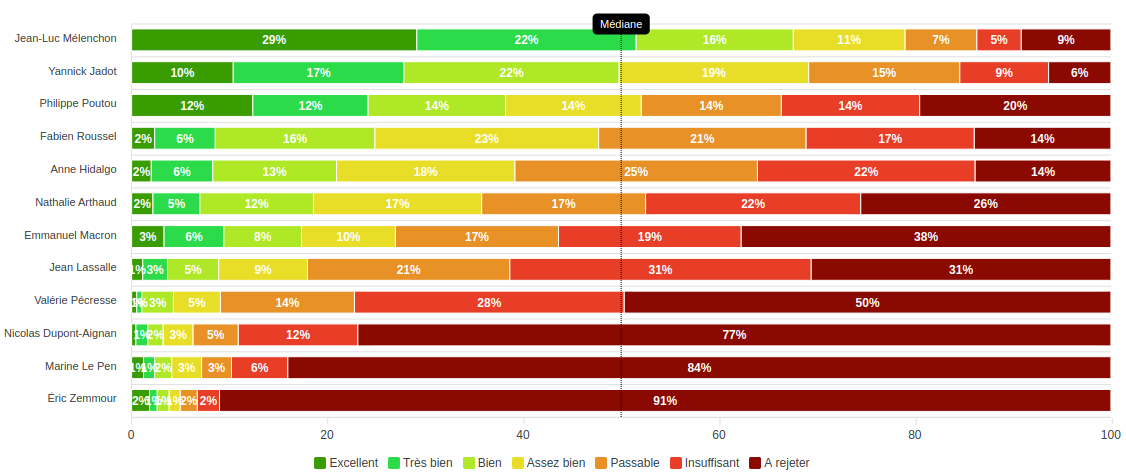
\includegraphics[scale=0.35]{data/profileUAV}
		\label{fig:distributionUAV}
	\end{figure}
	
	The grade vector associated to the candidate Jean-Luc Mélenchon is composed for: $29\%$ of Excellent grades, $22\%$ of Very good, $16\%$ of Good, $11\%$ of Average, $7\%$ of Mediocre, $5\%$ of Inadequate and for $9\%$ of To be rejected.
	Because it is the winner of the complete profile this alternative will be our $j_0$ and its complete grade vector will be formed following the same proportions: $29\%$ of $\delta_7$, $22\%$ of $\delta_6$, $16\%$ of $\delta_5$, $11\%$ of $\delta_4$, $7\%$ of $\delta_3$, $5\%$ of $\delta_2$ and for $9\%$ of $\delta_1$.
	We follow the same reasoning for the other grade vectors in order to have the complete profile.
	
	Given $m=12$ alternatives we fix a value of $n$ and see what is the probability that $j_0$ is not in $K$ for $k$ from $1$ to $5$. Using the same reasoning as in the previous experiment we repeat this a total of $1,000,000$ times and we average over the probability. After that we increase $n$ and repeat the same experiment. We note that the probability decreases dramatically as $n$ increases so, although we varied $n$ from $10$ to $1500$, in \Cref{fig:MJelicitationUAV} we show the results only for a limited number of $n$ values.
	\Cref{tab:MJelicitationUAV} shows the data for the same values of $n$, the complete dataset can be found at \url{https://github.com/xoxor/elicitationMJ}. We see that when we have $n=50$ voters by asking $k=3$ questions per voter already we have an almost zero probability of not electing $j_0$. This result is obtained by asking $2$ questions per voter when $n=100$ and $1$ question when $n=500$.
	
	These results suggest that in small profiles with few voters this method can pose a serious risk of not electing the "correct" alternative unless many questions are asked. This risk, however, is almost absent for elections in which a large number of voters are involved. Although we cannot use these findings to reach a definite conclusion, working in this direction might help in the formulation of a more comprehensive result.
	
	\begin{figure}
		\centering
		\caption{Average probability of missing the winner using a real case distribution of preferences, given $m=12$ for $n\in \{10,25,50,100,250,500\}$ and $k\in \intvl{1,5}$.}
		\label{fig:MJelicitationUAV}
		\begin{tikzpicture}[scale=1.2]
			\pgfplotsset{
				every axis legend/.append style={
					at={(0.5,1.1)},
					anchor=south
				},
			}
			\begin{axis}[
				%	y=8,
				xlabel=$k$,
				ylabel=Avg. Prob. of Miss.,
				table/col sep=comma,
				legend columns=3,
				%	ytick={0,2,4,6,8,10},
				%	xtick distance=10,
				%	ytick distance=2,
				%	xtick pos=left,
				ymajorgrids=true,
				ytick style={draw=none},
				ymin=0,
				ymax=0.8,
				xmin=1,
				xmax=5,
					legend style={font=\scriptsize}
				]
				
				\addlegendimage{mark=halfsquare right*,brown,mark size=2}
				\addlegendimage{mark=diamond*,red,mark size=2}
				\addlegendimage{mark=pentagon*,cyan,mark size=2}
				\addlegendimage{mark=halfcircle*,violet,mark size=2}
				\addlegendimage{mark=*,pink,mark size=2}
				\addlegendimage{mark=triangle*,green,mark size=2}
				\addlegendimage{mark=halfsquare left*,blue,mark size=2}
				\addlegendimage{mark=square*,teal,mark size=2}
				\addlegendimage{mark=halfsquare*,magenta,mark size=2}
				
				
				\addplot[thick, mark=halfsquare right*, mark size = {2}, mark indices = {3}, brown] table [x=k, y=p10]{data/electiontableFig.dat};
				\addlegendentry{n=10}
				\addplot[thick, mark=diamond*, mark size = {2}, mark indices = {3}, red] table [x=k, y=p25]{data/electiontableFig.dat};
				\addlegendentry{n=25}
				\addplot[thick, mark=pentagon*, mark size = {2}, mark indices = {2}, cyan] table [x=k, y=p50]{data/electiontableFig.dat};
				\addlegendentry{n=50}
				\addplot[thick, mark=halfcircle*, mark size = {2}, mark indices = {2}, violet] table [x=k, y=p100]{data/electiontableFig.dat};
				\addlegendentry{n=100}
				\addplot[thick, mark=*, mark size = {2}, mark indices = {1}, pink] table [x=k, y=p250]{data/electiontableFig.dat};
				\addlegendentry{n=250}
				\addplot[thick, mark=triangle*, mark size = {2}, mark indices = {1}, green] table [x=k, y=p500]{data/electiontableFig.dat};
				\addlegendentry{n=500}
%				\addplot[thick, mark=halfsquare left*, mark size = {2}, mark indices = {1}, blue] table [x=k, y=p1000]{data/electiontableFig.dat};
%				\addlegendentry{n=1000}
%				\addplot[thick, mark=square*, mark size = {2}, mark indices = {1}, teal] table [x=k, y=p1500]{data/electiontableFig.dat};
%				\addlegendentry{n=1500}
				
			\end{axis}
		\end{tikzpicture}
	\end{figure}
	
	
	\begin{table}
		\centering
		\captionsetup{type=table}
		\caption{Average probability of missing the winner using a real case distribution of preferences, given $m=12$ for different values of $k$ and $n$.}
		\label{tab:MJelicitationUAV}
		\begin{tabular}{S[table-figures-integer=1, table-figures-decimal=0]S[table-figures-decimal=2]S[table-figures-decimal=2]S[table-figures-decimal=2]S[table-figures-decimal=2]S[table-figures-decimal=2]S[table-figures-decimal=2]}
			\toprule
			{$k$} & {avg $\mathcal{P}_{n=10}$} & {avg $\mathcal{P}_{n=25}$}& {avg $\mathcal{P}_{n=50}$}& {avg $\mathcal{P}_{n=100}$}& {avg $\mathcal{P}_{n=250}$} & {avg $\mathcal{P}_{n=500}$} \\
			\midrule		
			1	&	0.705851	&	0.495156	&	0.336408	&	0.167265	&	0.033418	&	0.004053	\\
			2	&	0.503269	&	0.218081	&	0.066655	&	0.008869	&	0.000117	&	0.00	\\
			3	&	0.339681	&	0.095145	&	0.008971	&	0.000149	&	0.00	&	0.00	\\
			4	&	0.184584	&	0.035866	&	0.000723	&	0.000001	&	0.00	&	0.00	\\
			5	&	0.069446	&	0.0099	&	0.000025	&	0.00	&	0.00	&	0.00	\\				
			\bottomrule
		\end{tabular}
	\end{table}
	
	\section{Conclusions}
		In this paper we analyzed a procedure proposed by the association \textit{Mieux Voter} and used in a real life application by \textit{LaPrimaire.org} for eliciting judgments of a set of voters over a set of alternatives.
		The procedure consists of randomly asking each voter to judge $k$ candidates on the $m$ available. The $k$ alternatives with the best medians are then presented to all voters in a second round of voting, and the best alternative is selected by \ac{MJ} as the winner.
		We have proven that given a complete profile it is possible to find an incomplete profile (such that a possible completion is equal to the considered profile) with a different winner from the complete profile.
		We also showed that the probability of this happening depends on the profile considered. 
		
		Moreover, we have performed experiments on profiles in which each grade vector has a randomly generated distribution of grade. Fixing the number of voters, we analyzed how much of the grade vector we must know in order for the probability missing the winner to be low. We have found that when knowing only the $20\%$ of the vector (thus after having asked $10$ questions) the probability of missing the winner is close to zero.
		We have also considered a profile created from the grade distribution of a real voting scenario. We have found that the probability of not selecting the winner of the complete profile greatly decreases as the number of voters increases, making this method suitable for elections with large numbers of voters but less appropriate for small profiles.
		
		Future work on this topic could investigate the manipulability of this elicitation process. Especially on the side of the "analyst" who is in charge of questioning voters and how she can potentially manipulate the outcome by asking particular questions to specific groups of voters. For example, if she knows that voters in a given electoral district tend to vote predominantly for a given party she may decide never to ask those voters about that party's candidate (or vice-versa depending on the party she favors). 
		
		Another step might involve the explainability of this process to voters. In fact, voters may find difficult to believe that judging only one person gives a good approximation of the result that would be obtained by asking for the full profile. Also, they may not appreciate judging a random candidate and not their favorite.
		
		The code to reproduce the experiments in this article and the files with the reported data are available at \url{https://github.com/xoxor/elicitationMJ}.
	

	\chapter{Compromising as an Equal-Loss Principle}
	\label{ch:compromise}
		%!TeX root= ../thesis.tex

\begin{abstract}
A social choice rule aggregates the preferences of a group of individuals over a set of alternatives into a collective choice. The literature admits several social choice rules whose recommendations are supposed to reflect a compromise among individuals. We observe that all these compromise rules can be better described as \emph{procedural compromises}, i.e., they impose over individuals a willingness to compromise but they do not ensure an outcome where everyone has effectively compromised. We revisit the concept of a compromise in a collective choice environment with at least three individuals having strict preferences over a finite set of alternatives. Referring to a large class of spread measures, we view the concept of compromise from an \emph{equal loss} perspective, favoring an outcome where every voter concedes as equally as possible. As such, being a compromise may fail Pareto efficiency, which we ensure by asking voters to concede as equally as possible among the Pareto efficient alternatives. We show that Condorcet consistent rules, scoring rules (except antiplurality) and Brams-Kilgour compromises (except fallback bargaining) all fail to ascertain an outcome which is a compromise. A slight restriction on acceptable spread measures suffices to extend the negative result to antiplurality and fallback bargaining.
This failure also prevails for social choice problems with two individuals: all well-known two-person social choice rules of the literature, namely, fallback bargaining, Pareto and veto rules, short listing and veto rank, fail to pick ex-post compromises. We conclude that there is a need to propose and study rules that satisfy this equal loss, or outcome oriented, notion of a compromise.
\end{abstract}

\section{Introduction}
\label{sec:introduction}
In a typical social choice problem, several individuals express their preferences over a set of alternatives and one shall be picked as the collective outcome. Although the literature admits several \acp{SCR} with different properties, there is a common understanding that collective choices must reflect “compromises”. One of the first to explicitly refer to a \ac{SCR} as a compromise is \citet{Sertel1986} introducing the \emph{majoritarian compromise}. This \ac{SCR}, further analyzed by \citet{Sertel1999}, is a rediscovery of a method suggested by James W.\ Bucklin at the beginning of the \nth{20} century \citep{Erdelyi2015}. Starting from everyone’s ideal alternative, it falls back to the voters’ second, third and more generally $k$-\emph{th} best, until one of the alternatives considered appears among the first $k$ best for a majority. \citet{Brams2001} generalize this concept and introduce a class of \acp{SCR} called $q$\emph{-approval fall-back bargaining}, where $q$ is the required quantity of support that can vary from a single voter up to unanimity. Different choices of $q$ lead to different \acp{SCR}. Considering $n$ voters, the choice of $q=1$ corresponds to the plurality rule, $q=\ceil{\frac{n}{2}}$ is closely related, but not identical, to the majoritarian compromise and $q=n$ represents a bargaining procedure called \emph{fall-back bargaining}, which has been further analyzed by \citet{Kibris2007} and \citet{Congar2012}. We will refer to these rules as \ac{BK} compromises with threshold q.

As \citet{OezkalSanver2004} discuss, the concept of compromising is mostly understood as the trade off between the number of voters supporting an alternative (i.e., the quantity of support) and the distance of that alternative from the supporters’ ideal alternative (i.e., the quality of support). This trade off, which is explicit for $q$-approval fall-back bargaining, is also the basis for several other \acp{SCR} such as the \emph{median voting rule} proposed by \citet{Bassett1999} and further analyzed by \citet{Gehrlein2003} or the \emph{Condorcet practical method} described by \citet{Nurmi1999}. \Citet{Merlin2019} identify and analyze a large class of \emph{compromise rules} that explore this trade off.

One can argue that a collective choice \emph{per se} implies a compromise. After all, except extreme cases such as dictatorships,
a \acp{SCR} operates on the principle that all voters could fall back from their ideal position. Whether all voters effectively do fall back and whether this fall is “equal among voters” is the subject of our analysis. In what follows, we will present examples where they do not, which could be considered counter to the spirit of compromising. \footnote{This objection to the compromise nomenclature was raised by Jean-François Laslier during a CNRS workshop on compromising hosted by Istanbul Bilgi University in 2018.}

Consider the following example.
\begin{example}
	\label{ex:ex1}
	Let $N$ be a set of $n ≥ 3$ voters and $A$ a set of alternatives. $\linors$ represents the set of linear orders over $A$. Consider the following preference profile $P\in \linors^{N}$,
	\begin{center}
		$
		\begin{array}{cccc}
			\mathbf{1} \quad &c&b&a\\
			\mathbf{n-1} \quad &a&b&c\\
		\end{array}\quad ,
		$
	\end{center}
	which represents one individual who prefers $c$ to $b$, $b$ to $a$, hence $c$ to $a$; and $n-1$ individuals who prefer $a$ to $b$, $b$ to $c$, hence $a$ to $c$. At $P$, all \acs{BK} compromises, except when $q=n$ (i.e. fall-back bargaining that would select $b$) and $q=1$ (which would select both $a$ and $c$), will ignore the single voter and will pick $a$ as the collective outcome.
\end{example}

As a matter of fact, almost every \ac{SCR} will ignore this “marginal minority” and choose $a$ in this situation. While this choice is defensible on the grounds of qualified majoritarianism, it is questionable whether $a$ can be qualified as a compromise. Observe that $b$ receives unanimous support when each voter falls back one step from his ideal point. The question becomes more compelling when $a$ remains the collective choice even if the ignored group is much larger.

\begin{example}
	\label{ex:ex2}
	Consider the following preference profile with $n=100$:
	\begin{center}
		$
		\begin{array}{cccc}
			\mathbf{49} \quad &c&b&a\\
			\mathbf{51} \quad &a&b&c\\
		\end{array} \quad.
		$
	\end{center}
	When $q\in \intvl{1,\frac{n}{2}-1}$, all \acs{BK} compromises pick $\{a,c\}$, and, when $q=\frac{n}{2}$ and $q=\frac{n}{2}+1$, all \acs{BK} compromises pick $\{a\}$. Again, it does not appear as a compromise as almost half of voters reach their best alternative while the remaining half have to be contented with their worst one.
\end{example}

Observe that all these \acp{SCR} impose to voters a willingness to compromise, but do not effectively ensure a compromise as the collective choice. In fact, the term “compromise” in this literature refers to procedural compromises that differ from outcome oriented compromises, a conceptual distinction that seems to be overlooked in the literature.
This can also be viewed as a distinction between ex-ante and ex-post compromises, where the profile is the source of uncertainty.

To define an ex-post compromise, we adapt a concept of equal losses that considers allocation of continuous utilities. This principle is used for bargaining \citep{Chun1988, Chun1991} and bankruptcy problems \citep{Herrero2001}. 
We introduce two definitions of compromise. In both of them, we pick a spread measure that determines how equally a given vector of numbers is distributed and we propose to make a collective choice where voters give up from their ideal points “as equally as possible”. The difference between the two is that one, called \emph{egalitarian compromise}, insists on equality at the expense of Pareto efficiency while the other, called \emph{Paretian compromise}, is constrained to pick among the Pareto efficient alternatives. We show that Pareto efficient \acp{SCR} cannot ensure egalitarian compromises under any spread measure. We prove that several well-known \acp{SCR} such as Condorcet extensions, scoring rules, $q$-approval fall-back bargaining, all fail to be Paretian compromises under any spread measure. We provide examples for which being a Paretian compromise would necessitate to pick an alternative that is, although Pareto optimal, ranked very low by all voters. Such alternative would never be picked by any of the above-mentioned \acp{SCR}. 

We conclude that the equal-loss principle appears adequate for collective choice problems with at least three individuals, when egalitarianism, in the sense of conceding equally, is a major concern. Imagine a situation where the head of a laboratory needs to decide which project to fund and she asks for the preferences of the laboratory members. The workplace harmony is extremely important and, in order to avoid conflicts, the winning project must be equally supported by all members. 

Consider now a situation with only two voters. As the vast literature on the ultimatum game \citep{Werner2014} suggests, mutual consent is hard to obtain when one individual sees injustice at the levels of mutual losses. The equal-loss principle seems to be crucial in this new scenario.

Collective choice models with two individuals can be interpreted as bargaining or arbitration problems. While the bargaining interpretation necessitates an explicitly defined disagreement outcome \citep{Kibris2007}, the arbitration interpretation \citep{Sprumont1993} remains within the classical collective choice environment with no explicit disagreement outcome. In this paper, we consider the latter interpretation. 

Arbitration rules are thoroughly discussed by \citet{Barbera2020}. As prominent examples, we have fallback bargaining proposed by \citet{Brams2001}, the veto-rank and short listing procedures analysed by \citet{Clippel2014} and the Pareto-and-veto rules analysed by \citet{Laslier2020}. These models consider discrete alternatives which are not contained by the classical \citet{Nash1950} bargaining environment with convex utilities. We make the same assumption. However, as \citet{Mariotti1998} and \citet{Nagahisa2002} illustrate, the two worlds can be interconnected, as we do for the equal-loss principle of \citet{Chun1988} and \citet{Chun1991}. The arbitration environment presents an instance where the equal-loss principle could matter and it is rather surprising to discover that most interesting \acp{SCR} used as arbitration solutions fail to be Paretian compromises. 

The rest of the paper is organized as follows. \Cref{sec:notation} presents the basic notions and notation. \Cref{sec:compromise} introduces egalitarian compromises and Paretian compromises, two concepts that turn out to be logically incompatible. \Cref{sec:more2voters} shows that with at least three individuals, many \acp{SCR} fail to pick a compromise. \Cref{sec:2voters} considers the two-individual case, showing that most \acp{SCR} of the literature fail to pick compromises. \Cref{sec:conclusion} makes some concluding remarks. 

\section{Basic notions and notation}
\label{sec:notation}
Consider a finite set $N$ of individuals with $\#N=n\geq 2$ and a finite set $A$ of alternatives with $\#A=m\geq 3$. We write $\linors$ for the set of linear orders over $A$.
A generic element $\prefi$ of $\linors$ stands for a preference of $i\in N$. This implies that, given any $x ≠ y\in A$, precisely one of $x \prefi y$ and $y\prefi x$ holds while $x \prefi x$ holds for no $x\in A.$ Moreover, $x\prefi y$ and $y\prefi z$ implies $x\prefi z$ $\forall x,y,z\in A$.

A \emph{profile} $P: N → \linors$ associates with each individual $i \in N$ a preference $P(i) = {\prefi}$. A \emph{\acl{SCR}} (\acs{SCR}) is a mapping $f:\linors^{N} \rightarrow 2^{A} \setminus \{\emptyset \}$. 

We write $r_{\prefi}(x)=\#\{y\in A \suchthat y \prefi x\}+1$ for the \emph{rank} of $x\in A$ at ${\prefi} \in \linors$. We denote by $\lambda_{\prefi}(x)=r_{\prefi}(x)-1$ the loss in terms of ranks for $i\in N$ with preference $\prefi$, when $x$ is elected instead of the best alternative
for $i$. The mapping $\lambda_P: A → \alllosses$ assigns to each $x\in A$ the loss vector $\lambda_{P}(x)=(\lambda_{\prefi}(x))_{i\in N}$ induced by the election of $x$. The double brackets denote intervals in the integers.

We are interested in measuring the spread of loss vectors. To this end, we define a \emph{spread measure} $\sigma: \alllosses → \R_{+}$ as a function that associates a spread value to every possible loss
vector. We write $\Sigma$ for the set of spread measures $\sigma$ that satisfy, for every $l\in\alllosses$, $\sigma(l)=0 ⇔ l_{i}=l_{j}$ $\forall i,j\in N$. Thus, the spread of $l$ gets its lowest value $0$ in case of perfect equality and only in this case. Note that this condition incorporates the minimal requirement to identify a spread measure and leads to the largest set of spread measures one could define. As discussed in \Cref{sec:RestrictionOnSigma}, this flexibility has the advantage of making our results more general.

Given any distinct $x,y\in A$, we say that $x$ \emph{Pareto dominates} $y$ at $P \in\linors^{N}$ (or equivalently $y$ is \emph{Pareto dominated} by $x $ at $P$) iff $x\prefi y,\forall i\in N$. We denote by
$\paretopt(P)= \set{x \in A \suchthat \forall y \in A\setminus\{x\}, \exists i \in N \suchthat x \pref_i y}$ the set of \emph{Pareto optimal} alternatives at $P$.
A \ac{SCR} $f$ is \emph{Paretian} iff $f(P)\subseteq\paretopt(P)$ $\forall P\in\linors^{N}$.

\section{Egalitarian versus Paretian compromises}
\label{sec:compromise}
\subsection{Egalitarian compromises}
\label{sec:EgCompromise}
We let $\argmin_{X}(\sigma \circ \lambda_P) = \set{x \in X \suchthat \allowbreak{}\forall y \in X: \sigma(\lambda_P(x)) ≤ \sigma(\lambda_P(y))}$ denote the minimal elements of $X \subseteq A$ according to $(\sigma \circ \lambda_{P})$. In other words, $\argmin_{X}(\sigma\circ\lambda_{P})$ denotes the alternatives in X whose loss vectors are the most equally distributed according to the spread measure $\sigma$.

In what follows, we define some classes of \acp{SCR} that we are interested in analyzing. 


\begin{definition} A \ac{SCR} $f$ is an \emph{Egalitarian Compromise} (EC) iff \[\exists \sigma \in \Sigma \suchthat \forall P \in \linors^N \text{ we have }f(P) \subseteq \musigma.\]
\end{definition}

\begin{definition} A \ac{SCR} $f$ is \emph{Egalitarian Compromise Compatible} (ECC) iff \[\exists \sigma \in \Sigma \suchthat \forall P \in \linors^N \text{ we have } f(P) \cap \musigma \neq \emptyset.\]
\end{definition}

Under a \ac{SCR} that is EC (resp., ECC), \emph{all} (resp., \emph{some}) winners are among the alternatives with most equally distributed losses. Clearly, EC is a subclass of ECC. Perhaps less obviously, being ECC (or EC) is incompatible with being Paretian. This will be deduced from the following proposition, which will also be useful to prove other theorems.% \cref{th:incompatibility}.

\begin{proposition} \label{prop:muSigmaLast}
	For $n ≥ 2, m ≥ 3$, there exists a profile $P \in \linors^N$ and an alternative $a_m$ such that $\forall i \in N$: $r_{\prefi}(a_m)=m$, and such that $\forall \sigma \in \Sigma: \musigma = \set{a_m}$; hence, $\musigma \cap \paretopt(P) = \emptyset$.
\end{proposition}
\begin{proof}
	Consider the following profile $P$:
	\begin{center}
		$
		\begin{array}{cccccc}
			\mathbf{1} \quad &a_1&a_2&\dots&a_{m-1}&a_m\\
			\mathbf{n-1} \quad &a_{\pi_{(1)}}&a_{\pi_{(2)}}&\dots&a_{\pi_{(m-1)}}&a_m\\
		\end{array}
		$ \quad,
	\end{center}
	where $\pi$ is the following permutation over $\intvl{1, m-1}$:
	\[
	\pi(i) = 
	\begin{cases}
		i+1 & \text{if } i \in \intvl{1, m-2} \\
		1 & \text{if } i = m-1
	\end{cases} \quad .
	\]
	In $P$, $a_m$ is the only alternative such that $r_{\prefi}(a_m)$ is independent of $i$; hence, $\sigma(\lambda_P(a)) > 0$, $\forall a \in A\setminus \{a_m\}$, $\forall \sigma \in \Sigma$. Thus, the set $\musigma$ consists of the sole element $a_m$, and, because $a_m$ is Pareto dominated, $\musigma \cap \paretopt(P) = \emptyset$.
\end{proof}

Our main result for \cref{sec:EgCompromise} follows easily.
\begin{theorem} \label{th:nonParetian}
	For $n\geq 2, \ m\geq3$, no Paretian \ac{SCR} is ECC.
\end{theorem}
\begin{proof}
	Proving this amounts to show that $\forall \sigma \in \Sigma, \exists P \in \linors^N \suchthat \paretopt(P) \cap \musigma = \emptyset$. Suffices to use \cref{prop:muSigmaLast}, which asserts that there exists a profile $P$ such that $\forall \sigma \in \Sigma: \musigma \cap \paretopt(P) = \emptyset$.
\end{proof}

\subsection{Paretian compromises}
Having seen the tension for a \ac{SCR} being Paretian and ECC, we investigate the consequences of inverting the order of priorities by insisting that at least some of the winning alternatives are Pareto optimal, and considering the most equally distributed loss vectors among those.

We consider two classes of \acp{SCR}. 
Observe that $\mustar$ denotes the set of Pareto optimal alternatives whose loss vectors are the most equally distributed according to the spread measure $\sigma$.

\begin{definition} A \ac{SCR} $f$ is a \emph{Paretian Compromise} PC iff \[\exists \sigma \in \Sigma \suchthat \forall P \in \linors^N \text{ we have } f(P) \subseteq \mustar.\]
\end{definition}

\begin{definition} A \ac{SCR} $f$ is \emph{Paretian Compromise Compatible} PCC iff \[\exists \sigma \in \Sigma \suchthat \forall P \in \linors^N \text{ we have } f(P) \cap \mustar \neq \emptyset.\]
\end{definition}

Again, it is clear that PC is a subclass of PCC. It will also probably come with no surprise that for a \ac{SCR}, being PC is incompatible with being ECC, as being PC requires to be Paretian, which permits to use \cref{th:nonParetian}. On the other hand, it is less immediate that being EC is incompatible with
being PCC, because being PCC does not require to be Paretian. This is however true.

\begin{theorem} \label{th:incompatibility} 
	For $n ≥ 2, m ≥ 3$, no \ac{SCR} is both EC and PCC.
\end{theorem}
\begin{proof}	
	Considering the profile $P$ of \cref{prop:muSigmaLast}, with $a_m$ the alternative mentioned there, any EC $f$ and any $\sigma \in \Sigma$, suffices to prove that $f(P) \cap {\mustar[\sigma][P]} = \emptyset$.
	
	First, from \cref{prop:muSigmaLast} we have that
	$\set{a_m} \cap \paretopt(P) = \emptyset$, hence $\set{a_m} \cap$ \break $ {\mustar[\sigma][P]} = \emptyset$. 
	
	Second, because $f$ is EC, for some $\sigmatop$, $f(P) \subseteq {\musigma[\sigmatop][P]}$. Using \cref{prop:muSigmaLast} again, we see that ${\musigma[\sigmatop][P]} = \set{a_m}$, hence $f(P) = \set{a_m}$.
	
	That $f(P) \cap {\mustar[\sigma][P]} = \emptyset$ follows from these two facts.
\end{proof}

It is interesting to note that the incompatibility is not complete, however.

\begin{remark}
	For $n ≥ 2$, $m ≥ 3$, there exist \acp{SCR} that are both ECC and PCC, such as the \ac{SCR} that selects the whole set of alternatives at every profile. However, this \ac{SCR} fails to be Paretian, as is any \ac{SCR} that is ECC.
\end{remark}


\section{Which \acp{SCR} are compromises?}
\label{sec:more2voters}
In this section we assume $n\geq 3$ and leave the analysis of $n=2$ to the
next section.

\subsection{Condorcet consistent rules}

An alternative $x\in A$ is a \emph{Condorcet winner} at $P\in \linors^N$ iff for all $y\in A \setminus \set{x} $, $\#\set{i \in N \suchthat x \prefi y} >\#\set{i \in N \suchthat y \prefi x}$. So each profile admits
either no or a unique Condorcet winner. An \ac{SCR} $f$ is \emph{Condorcet
	consistent} iff $f(P)=$ $\left\{ x\right\} $ at each $P\in \linors^N$ that
admits $x$ as the (unique) Condorcet winner.

\begin{theorem} \label{th:condorcet}
	Let $n\geq 3$ and $m\geq 3$. A Condorcet consistent \ac{SCR} $f$ is neither ECC nor PCC.
\end{theorem}
\begin{proof}
	Consider the following profile $P$, where the dots represent the sequence $a_4$ to $a_m$:
	\begin{center}
		$
		\begin{array}{cccccc}
			\mathbf{n-1} \quad &a_1&a_2&a_3&\dots\\
			\mathbf{1} \quad &a_3&a_2&\dots&a_1\\
		\end{array}
		$ \quad.
	\end{center}
	
	Consider any Condorcet consistent \ac{SCR} $f$. Thus, $f(P)=\{a_1\}$. However, $\musigma=\mustar=\{a_2\}$ $\forall \sigma \in \Sigma$, so there exists a profile $P$ such that both $f(P)\cap \musigma$ and $f(P)\cap \mustar$ are empty.
\end{proof}

Note that Condorcet consistent rules need not be Paretian so the fact that they all fail ECC does not follow from \cref{th:nonParetian}. 

\subsection{Scoring rules}
\label{sec:scoringrules}
A \emph{score vector} is an $m-$tuple $w=(w_{1},\dots,$ $w_{m})\in \intvl{0, 1}^{m}$ with $w_{1}=1$, $w_{m}=0$ and $w_{i}\geq w_{i+1}$ $\forall i\in \intvl{1, m-1}$. Given a score vector $w$, we write $s^{w}(x,P)=\sum_{i\in N}w_{r_{\prefi}(x)}$ for the score of $x\in A$ at $P \in \linors^N$. Each vector $w$ identifies a \emph{scoring rule} $f^w_n$ defined as $f^w_n(P)=\left\{ x\in A:s^{w}(x,P)\geq s^{w}(y,P) \ \forall y\in A\right\}$ for every $P \in \linors^N$.

We first show that no scoring rule is ECC, for any value of $n$ and $m$ at least 3.

\begin{theorem}\label{th:srECC}
	Let $n\geq 3$ and $m\geq 3.$ No score vector $w$ induces a scoring rule $f^w_n$ that is ECC.
\end{theorem}
\begin{proof}
	Take any score vector $w$. Consider the profile $P$ of \cref{prop:muSigmaLast}. Observe that $\musigma=\{a_m\} \ \forall \sigma \in \Sigma $. However, as $w_{1}>w_{m}$, we have $s^{w}(a_{1},P)>s^{w}(a_{m},P)$ which implies $a_{m}\notin f^{w}(P)$.
\end{proof}

We call antiplurality score vector the vector $w$ such that $w_{i} = 1, \forall i \in \intvl{1, m-1}$, and $w_{m}=0$.

\begin{theorem}
	\label{th:AntSatsPCC}
	Let $m\geq 3$ and let $w$ be the antiplurality score vector. The \ac{SCR} $f_{n}^{w}$ satisfies PCC for all $n\geq 3$.
\end{theorem}
\begin{proof}
	Define $\bar\sigma \in \Sigma$ as, $\forall l \in \intvl{0,m-1}^N$: $\bar\sigma(l) = 1$ iff $\exists i, j \in N \suchthat l_i ≠ l_j$; $\bar\sigma(l) = 0$ otherwise.
	We show the non-emptiness of $f^w_n(P) \cap \mustar[\bar\sigma]$ for any profile $P$.
	
	Let $k = \min_{\paretopt(P)} \set{(\bar\sigma \circ \lambda_P)(x)}$ be the minimal value attained by $\bar\sigma \circ \lambda_P$ over $\paretopt(P)$. By construction of $\bar\sigma$, $k$ equals either $0$ or $1$.
	
	For $k = 1$, take any $x \in f^w_n(P) \cap \paretopt(P)$. This intersection is non-empty because whenever the antiplurality rule picks a Pareto dominated alternative $z$, it also picks all alternatives which Pareto dominate $z$.
	By definition of $\bar\sigma$, $\bar\sigma(x) ≤ 1$, hence, $x \in \mustar[\bar\sigma]$.
	%	We then have that $x \in \mustar[\bar\sigma]$ as by definition of $\bar\sigma$, $\bar\sigma(x) ≤ 1$.
	
	For $k = 0$, take any $x \in \mustar[\bar\sigma]$. As $\bar\sigma (\lambda _{P}(x))=0$, we have, $\forall i, j \in N$: $\lambda_i^P(x) = \lambda_j^P(x)$, hence, $\forall i, j \in N$: $r_{\succ_i}(x) = r_{\succ_j}(x)$. 
	The case $r_{\succ_i}(x) = m, \forall i \in N$ is ruled out by $x \in \paretopt(P)$. Hence, $r_{\succ_i}(x) ≤ m - 1, \forall i \in N$, hence, $x \in f^w_n(P)$.
\end{proof}

It is worth noting that the antiplurality rule $f_{n}^{w}$ is not Paretian, hence fails PC  for all $n\geq 3$. This can be seen by picking a unanimous profile $P \in \linors^{N}$ with $a_{1}\prefi a_{2}\prefi \dots \prefi a_{m}$ $\forall i\in N$, where $\mustar=\left\{ a_{1}\right\} \forall \sigma \in \Sigma $ while $f_{n}^{w}(P)=A \setminus \left\{ a_{m}\right\}$.

\begin{theorem}
	\label{th:srPCC}
	Let $m\geq 3.$ Take any score vector $w$ which is not the antiplurality score vector. For some $n ≥ 3$, the \ac{SCR} $f_{n}^{w}$ fails PCC.
\end{theorem}

\begin{proof}
	Take any $m\geq 3$ and any score vector $w$ that is not the antiplurality score vector; therefore, $w_{m-1}<1$. Pick any $n$ such that $n ≥ m - 1$ and $n > \frac{1}{1 - w_{m - 1}}$. Consider a profile $P \in \linors^N$ conforming to
	
	\begin{center}
		$
		\begin{array}{cccccc}
			i = 1 \quad & a_2 & … & a_m & a_1\\
			2 ≤ i ≤ m - 2 \quad & a_1 & … & a_m & a_i\\
			m - 1 ≤ i ≤ n \quad & a_1 & … & a_m & a_{m-1}\\
		\end{array}
		$\quad,
	\end{center}
	where all alternatives except $a_m$ appear at least once in the last rank.
	Thus, for every $\sigma \in \Sigma$, we have 
	$\sigma (\lambda _{P}(x))>0$ $\forall x\in A \setminus \left\{ a_{m}\right\}$
	while
	$\sigma (\lambda_{P}(a_{m}))=0$. 
	Moreover, $a_{m}\in \paretopt(P)$. Thus, $\mustar=\left\{ a_{m}\right\} $ $\forall \sigma \in \Sigma $. On the other hand, $s^{w}(a_{1}; P)=n-1$, $s^{w}(a_{m}; P)=n\cdot w_{m-1}$ and
	as $n > \frac{1}{1 - w_{m - 1}}$ (or, equivalently, $n - 1 > n w_{m - 1}$), we have $s^{w}(a_{1}; P)>s^{w}(a_{m};$ $P)$,
	establishing $a_{m}\notin f^{w}(P)$, thus $f^{w}(P)\cap \mustar=\emptyset $ $\forall \sigma \in \Sigma $.
\end{proof}

\subsection{\acs{BK} compromises}
\label{sec:BKn3}
Given any $k\in \intvl{1, m}$, we write $n_{k}(x,P)=\#\{i\in
N\mid r_{\prefi}(x)\leq k\}$ for the \emph{$k$-support} that $x$ gets at $P$, that is, the number of individuals for whom the rank of alternative $x\in A$ is lower than or equal to $k$ in the profile $P \in \linors^N$.
Note that $n_{k}(x,P)\in \intvl{1, n}$ is non-decreasing on $k$ and $n_{m}(x,P)=n.$ For each $q\in \intvl{1,n}$, we define $\rho_{q}(x,P)=\min \{k\in \intvl{1,m} \suchthat n_{k}(x,P)\geq q\}$ as the minimal rank $k$ at which the $k$-support that $x$ gets at $P$ is at least $q$. We
write $\rho _{q}(P) = \min_{x \in A} \set{\rho_{q}(x, P)}$ for the minimal rank $k$ at which the $k$-support that some alternative gets at $P$ is at least $q$. A \emph{\ac{BK} compromise with threshold }$q$ is the
\ac{SCR} $f_{q}$ defined for each $P\in \linors^N$ as $f_{q}(P)=\{x\in A \suchthat n_{\rho _{q}(P)}(x,P)\geq q\}$.
We can also define a tie breaking version of the \acs{BK} compromise where among the winners only the alternatives with the greatest support are selected: $f'_{q}(P)=\{x\in A \suchthat n_{\rho _{q}(P)}(x,P)\geq n_{\rho _{q}(P)}(y,P), \forall y\in A\}$

We first consider the \acs{BK} compromise with threshold $q=n$, $f_n$, which corresponds to the rule also known as \textit{fallback bargaining} \citep{Brams2001}.

\begin{theorem}
	\label{th:FBsatsPC}
	Let $n\geq 3$ and $m\geq 3.$ The \acs{BK} compromise $f_{n}$ satisfies PC.
\end{theorem}

\begin{proof}
	Define $\bar{\sigma } \in \Sigma$ as, $\forall l \in \intvl{0,m-1}^N$: $\bar\sigma(l) = 1$ iff $\exists i, j \in N \suchthat l_i ≠ l_j$; $\bar\sigma(l) = 0$ otherwise.
	Considering any $x \in f_n(P)$, let us show that $x \in \mustar[\bar{\sigma}]$. Because $x \in f_n(P)$, $x \in \paretopt(P)$, and therefore, suffices to show that $\forall y \in \paretopt(P)$, $\bar{\sigma}(\lambda_P(y)) ≥ \bar{\sigma}(\lambda_P(x))$. Given the choice of $\bar{\sigma}$, picking any $y \in \paretopt(P)$ with $y≠x$, suffices to show that $\bar{\sigma}(\lambda_P(y)) = 1$, equivalently, that $\exists i, j \in N \suchthat r_{\prefi}(y) ≠ r_{\pref_j}(y)$. 
	Because $x \in f_n(P)$, $\rho_n(P) = \rho_n(x, P) = \max_{N} r_{\prefi}(x)$.
	It follows from $\rho_n(P) = \min_{z \in A} \set{\rho_n(z, P)}$ that $\rho_n(y, P) ≥ \rho_n(x, P)$, thus, $\exists i \in N \suchthat r_{\prefi}(y) ≥ \rho_n(P)$. 
	Also, $y \in \paretopt(P)$ implies that $\exists j \in N \suchthat r_{\pref_j}(y) < r_{\pref_j}(x)$, thus $\exists j \in N \suchthat r_{\pref_j}(y) < \rho_n(P)$. 
	Therefore, $r_{\prefi}(y) ≠ r_{\pref_j}(y)$.
\end{proof}

\begin{theorem}
	\label{th:FBfailsECC}
	Let $n\geq 3$ and $m\geq 3.$ The BK compromise $f_{n}$ fails ECC. 
\end{theorem}
\begin{proof}
	As $f_{n}$ is Paretian, the proof comes straightforward from \cref{th:nonParetian}.
\end{proof}

\begin{theorem}
	\label{th:BKthreshold}
	Let $n\geq 3$ and $m\geq 3.$ A BK compromise $f_{q}$ with threshold $q \in \intvl{1, n-1}$ is neither ECC nor PCC.
\end{theorem}
\begin{proof}
	%Take any $n\geq 3$ and $m\geq 3.$ Let $A=\left\{ a_{1},\text{ }a_{2,}...
	%\text{ }a_{m}\right\} $. Pick some $q\in \left\{ 1,...,n\right\} $ and
	%consider the BK compromise $f_{q}$. 
	Consider the following profile $P$ (also used in the proof of \cref{th:condorcet}), where the dots represent the sequence $a_4$ to $a_m$:
	\begin{center}
		$
		\begin{array}{cccccc}
			\mathbf{n-1} \quad &a_1&a_2&a_3&\dots\\
			\mathbf{1} \quad &a_3&a_2&\dots&a_1\\
		\end{array}
		$\quad.
	\end{center}
	When $q=1$ we have that $f_{1}(P)=\{a_1,a_3\}$ and when $q \in \intvl{2, n-1}$ we have that $f_{q}(P)=\{a_1\}$. Because $\sigma(\lambda_P(a_2)) = 0$ and $\sigma(\lambda_P(a_1)) > 0$ and $\sigma(\lambda_P(a_3)) > 0$, neither $\musigma$ nor $\mustar$ contain $a_1$ nor $a_3$ for any $\sigma \in \Sigma$. 

	Note that for $q \in \intvl{1, n-1}$ we have that $f'_{q}(P)=\{a_1\}$ since the tie breaking version of the \acs{BK} compromise selects the alternatives with the greatest support. This version of the rule was used in the proof for \Cref{th:BKthreshold} published by \citet{Cailloux2022}.
	%Remzi’s proof
	%Take any $n\geq 3$ and $m\geq 3.$ Let $A=\left\{ a_{1},\text{ }a_{2,}...%
	%\text{ }a_{m}\right\} $. Pick some $q\in \left\{ 1,...,n\right\} $ and
	%consider the BK compromise $f_{q}$. Consider the profile $P\in \linors^{N}$ such that 
	%$a_{1}\succ _{i}a_{2}\succ _{i}...\succ _{i}a_{m}$ $\forall i\in N\diagdown
	%\left\{ n\right\} $ and $a_{\pi (1)}\succ _{n}a_{\pi (2)}\succ _{n}...\succ
	%_{n}a_{\pi (m)}$ where $\pi $ is a bijection on $\left\{ 1,\text{ }2,...,%
	%\text{ }m\right\} $ with $\pi (1)=3$, $\pi (2)=2,\pi (3)=1$, $\pi (i)=i+1$ $%
	%\forall i\in \left\{ 4,...,\text{ }m-1\right\} $ and $\pi (m)=4 $, we have $%
	%f_{q}(P)=\left\{ a_{1}\right\} $ while $\mu _{\sigma }(P)=\mu _{\sigma
	%}^{\ast }(P)=\left\{ a_{2}\right\} $ $\forall \sigma \in \Sigma $.
\end{proof}

\subsection{Restrictions on sigma}
\label{sec:RestrictionOnSigma}
The perfect equality recognition condition we adopt for spread measures, i.e., that the spread gets its lowest value $0$ in case of perfect equality and only in this case, is very basic. Unless this condition is violated, $\Sigma$ is the largest set of spread measures we could conceive. On the other hand, it is possible to let $\Sigma$ shrink by imposing additional conditions over spread measures. Nevertheless, as the satisfaction of PC, PCC, EC, or ECC requires the existence of a spread measure, all of our negative results, namely, those expressed by Theorems \ref{th:nonParetian}, \ref{th:incompatibility}, \ref{th:condorcet}, \ref{th:srECC}, \ref{th:srPCC}, \ref{th:FBfailsECC} and \ref{th:BKthreshold} prevail when $\Sigma$ is restricted. In a similar vein, the positive results in Theorems \ref{th:AntSatsPCC} and \ref{th:FBsatsPC} risk to be lost with additional conditions over spread measures.
Indeed, this section shows that a mild restriction removes the positive results concerning the only two rules that we found to be compatible with any of our compromise concepts.

\begin{definition}
	\label{def:conditionC}
	Given any $m\geq4$ and $n\geq \max\{4,m-1\}$, we say that a spread measure $\sigma$ satisfies condition $C_{m,n}$ iff we have $\sigma(m-3, m-1, m-2, \dots, m-2) < \sigma(m-2, m-3, \dots, 1, 0, \dots, 0)$.
\end{definition}

As both vectors are $n$ dimensional, the term $m-2$ repeats $n-2$ times in the first vector and the term $0$ repeats $n-m+2$ times in the second vector.

This condition imposes a very reasonable requirement on spread measures for large values of $m$ and $n$. Asking for $\sigma(1,3,2,2)$ to be smaller than $\sigma(2,1,0,0)$ is demanding while asking for $\sigma(5,7,6,6,6,6,6)$ to be smaller than $\sigma(6,5,4,3,2,1,0)$ reflects a mild assumption. In any case, as we state below, several well-known spread measures of the literature (see \citet{Allison1978} for a comprehensive account) satisfy \cref{def:conditionC}. Letting $\bar{l} = \sum_{i=1}^{n} l_i / n$ denote the arithmetic mean of the values of $l = (l_1, …, l_n)$, we consider the following measures:

\begin{itemize}
	\item the mean absolute difference $\sigma_{mad}(l)= \frac{1}{n^2} \sum_{i=1}^{n}\sum_{j=1}^{n}|l_i-l_j|$;
	\item the average absolute deviation $\sigma_{ad}(l)= \frac{\sum_{i=1}^{n}|l_i-\bar{l}|}{n}$;
	\item the standard deviation $\sigma_{sd}(l)= \sqrt{\frac{\sum_{i=1}^{n}(l_i-\bar{l})^2}{n}}$;
	\item the Gini coefficient $\sigma_{G}(l)= \frac{\sum_{i=1}^{n}\sum_{j=1}^{n}|l_i-l_j|}{2 \cdot n \cdot \sum_{i=1}^{n} l_i}$.
\end{itemize} 

\begin{remark}
	\label{prop:spreadMeas}
	We checked experimentally that $\sigma_{mad}$, $\sigma_{ad}$, $\sigma_{sd}$ and $\sigma_{G}$ all satisfy condition $C_{m,n}$, for $m \in \intvl{4,1000}$ and $n \in \intvl{b, 1000}$ where $b = \max\{4,m-1\}$.
\end{remark}

%A \emph{spread measure} $\sigma: \alllosses → \R_{+}$ satisfies condition gamma iff  $\sigma (m-3,$ $m-1,m-2,...,$ $m-2)$ <$\sigma(m-2,$ $m-1,...1,$0, $\ 0)$.
%			(\lambda_{P}(y))$ that associates a spread value to every possible loss
%vector. We write On the other hand, $\lambda
%			^{P}(x)=(m-3,$ $m-1,m-2,...,$ $m-2)$ and $\lambda_{P}(y)=(m-2,$ $m-1,,...1,$
%			$0,$ $\ 0)$.

We write $\Sigma^{C_{m,n}} \subseteq \Sigma$ for the set of spread measures that satisfy condition $C_{m,n}$. 
\begin{theorem} 
	\label{th:3votRestriction}
	For all $m\geq 4$, $n\geq \max\{4,m-1\}$, under $\Sigma^{C_{m,n}}$,
	\begin{itemize}
		\item [1)] $f_n^{w}$ fails PCC when $w$ is the antiplurality score vector;
		\item [2)] the \acs{BK} compromise  $f_n$ fails PCC.
	\end{itemize}
\end{theorem}
\begin{proof}
	Given any $\sigma \in \Sigma^{C_{m,n}}$, let us show that there exists a profile $P$ such that $f_n^{w} \cap \mustar = \emptyset$ and $f_n \cap \mustar = \emptyset$. To that aim, consider some $x,y\in A$ and some $P\in \linors^{N}$ with $r_{\prefi[1]}(x)=m-2$, $r_{\prefi[2]}(x)=m,$ $r_{\prefi}(x)=m-1$ $\forall i\in N \setminus \left\{ 1, 2\right\}$, and $r_{\prefi}(y)=m-i$ $\forall i\in \intvl{1,m-1}$, $r_{\prefi[j]}(y)=1$ $\forall j\in \intvl{m,n}$. Moreover, for each $z\in A \setminus \left\{ x,y\right\} $, let $r_{\prefi[i]}(z)=m$ for some $i\in N$. 
	
	Note that $f_n^{w}(P) = f_{n}(P) = \set{y}$. On the other hand, $\lambda_{P}(x)=(m-3, m-1,m-2,\dots,m-2)$ and $\lambda_{P}(y)=(m-2, m-3,\dots,1,0, \dots, 0)$. As $\sigma(\lambda_{P}(x)) < \sigma(\lambda_{P}(y))$ (because $\sigma \in \Sigma^{C_{m,n}}$), we see that $y\notin \mustar$.
\end{proof}

\section{Two-voters case}
\label{sec:2voters}
In addition to \emph{fallback bargaining (FB)} \citep{Brams2001} (defined in \cref{sec:BKn3}), we consider three prominent solutions of the literature.

\emph{Pareto-and-Veto rules (PV)} \citep{Moulin1983, Abreu1991, Laslier2020} distribute a veto power of $v_1$ and $v_2$ alternatives to voters 1 and 2, respectively, with $v_1+v_2=m-1$. So, every voter $i=1,2$ (simultaneously) vetoes his worst $v_i$ alternatives. The \ac{SCR} picks all non-vetoed and Pareto optimal alternatives.

The \emph{Veto-Rank mechanism (VR)} is commonly used in the selection of arbitrators \citep{Clippel2014}. Given a list of $m$ (odd) alternatives (that are candidates to be arbitrators), each of the two voters (that are the two parties that must agree on an arbitrator) simultaneously vetoes his worst $\frac{m-1}{2}$ alternatives. The selected alternatives are the ones with the highest Borda score among the non-vetoed alternatives.

Again within the context of selecting arbitrators, \citet{Clippel2014} propose and analyze \emph{Shortlisting (SL)} where one of the two parties starts by vetoing her worst $\frac{m-1}{2}$ alternatives ($m$ being odd), and then the second party chooses her best alternative out of the remaining ones. As the outcome of the procedure depends on the party that starts, symmetry among players is ensured by defining the solution as the union of the two outcomes where one and the other party starts.


\begin{definition}
	Given any $m \geq 7$, a spread measure $\sigma \in \Sigma$ satisfies condition $D_m$ iff 
	$\sigma(\ceil{\frac{m}{2}}, \ceil{\frac{m}{2}} - 2) < \sigma(0, \ceil{\frac{m}{2}} - 1)$ and 
	$\sigma(\ceil{\frac{m}{2}} - 2, \ceil{\frac{m}{2}}) < \sigma(\ceil{\frac{m}{2}} - 1, 0)$.
\end{definition}

For $m=7$ the condition requires $\sigma(4, 2) < \sigma(0, 3)$ and $\sigma(2, 4) < \sigma(3, 0)$ which is reasonable in our context. When the value of $m$ is larger, the condition appears even more convincing. As $m$ grows, the distance between $0$ and $\ceil{\frac{m}{2}} - 1$ grows, while the distance between $\ceil{\frac{m}{2}}$ and $\ceil{\frac{m}{2}} - 2$ remains constant. Requiring, for example, the spread of $(15, 13)$ to be smaller than the spread of $(0, 14)$ is very reasonable.

We write $\Sigma^{D_{m}} \subseteq \Sigma$ for the set of spread measures that satisfy condition $D_{m}$. 

\begin{theorem} \label{th:2votPCC}
	Let $m \geq 7$. Under $\Sigma^{D_{m}}$, FB and PV fail PCC. Furthermore, when $m$ is odd, VR and SL also fail PCC.
\end{theorem}
\begin{proof}
	Take any $m \geq 7$ and any $\sigma \in \Sigma^{D_m}$. Define $\alpha = \ceil{\frac{m}{2}} - 1$ and $\beta = \ceil{\frac{m}{2}} - 2$. It follows from $\sigma \in \Sigma^{D_{m}}$, that $\sigma(\alpha + 1, \beta) < \sigma(0, \beta + 1)$ and $\sigma(\beta, \alpha + 1) < \sigma(\beta + 1, 0)$.
	For $m$ odd, note that $\alpha + \beta + 2 = m$ and consider the profile $P$ where voter $i_1$ has the preference $x \succ a_1 \succ … \succ a_\alpha \succ y \succ b_1 \succ … \succ b_\beta$ and voter $i_2$ has the preference $b_1 \succ … \succ b_\beta \succ y \succ x \succ a_1 \succ … \succ a_\alpha$. For $m$ even, note that $\alpha + \beta + 3= m$, and define the profile $P$ in the same way, except that a supplementary alternative $z$ is added at the bottom of both rankings.
	
	Note that $\sigma(\lambda_{P}(y)) = \sigma(\alpha + 1, \beta)$ and that $\sigma(\lambda_{P}(x)) = \sigma(0, \beta + 1)$. 
	Therefore, $\sigma(\lambda_{P}(y)) < \sigma(\lambda_{P}(x))$. As $y$ is not Pareto-dominated, an \ac{SCR} that uniquely picks $x$ at $P$ cannot be PCC. In a similar vein, at the profile $P'$ which is obtained by the inversion of the preferences of $i_1$ and $i_2$ at $P$, an \ac{SCR} that is PCC cannot pick $x$ uniquely.	
	
	The proof will be concluded by showing that FB, PV, and (when $m$ is odd) VR and SL all pick only $x$ at $P$ or at $P'$.
	
	We readily see that FB picks only $x$ at $P$ (and at $P'$) since $x$ is the first alternative which reaches the unanimous consent.
	For PV, let $v_{i_1} ≥ v_{i_2}$ (thus $v_{i_1} ≥ \ceil{\frac{m-1}{2}} ≥ \ceil{\frac{m-2}{2}} = \beta + 1$ and $v_{i_2} ≤ \floor{\frac{m - 1}{2}} = \ceil{\frac{m - 2}{2}} = \alpha$), and consider the profile $P$. Observe that the first voter vetoes at least $y$ and every $b_j$ ($1 ≤ j ≤ \beta$) while no voter vetoes $x$. As $x$ Pareto-dominates every $a_j$ ($1 ≤ j ≤ \alpha$), PV picks only $x$ at $P$. When $v_{i_2} ≥ v_{i_1}$, a similar reasoning yields that PV picks only $x$ at $P'$.
	
	Now let $m$ be odd.
	
	For VR, a reasoning similar to the one applied to PV yields $x$ as the unique choice at $P$: each voter vetoes her worst $\frac{m-1}{2}$ alternatives, thus $i_1$ vetoes $y$ and every $b_j$ ($1 ≤ j ≤ \beta$) and $i_2$ vetoes every $a_j$ ($1 ≤ j ≤ \alpha$). The alternative $x$ is the only non-vetoed alternative, so it is selected as the sole winner.
	
	Finally, SL also picks $x$, as it is the unique winner no matter which voter starts the veto phase. If $i_1$ starts, $y$ and every $b_j$ ($1 ≤ j ≤ \beta$) get vetoed, then $i_2$ chooses her best alternative out of the remaining ones which is $x$. If $i_2$ starts, every $a_j$ ($1 ≤ j ≤ \alpha$) get vetoed, then $i_1$ chooses her best alternative which is $x$. 
\end{proof}



\section{Concluding remarks}
\label{sec:conclusion}
We define an ex-post compromise as an outcome where individuals give up as equally as possible from their ideal points. 
With three or more individuals, several well known \acp{SCR} fail to pick ex-post compromises, under any reasonable meaning attributed to “giving up equally”. 
Our findings cover Condorcet extensions and scoring rules but also \acs{BK} compromises, which impose a willingness to compromise without ensuring a compromised outcome.
In particular we find that: no Condorcet procedure is ECC or PCC (\Cref{th:condorcet}), no scoring rule is ECC (\Cref{th:srECC}) or PCC except for the antiplurality rule (\Cref{th:AntSatsPCC,th:srPCC}), \acs{BK} compromises are neither ECC or PCC (\Cref{th:BKthreshold,th:FBfailsECC}) except for fallback bargaining that is PC (\Cref{th:FBsatsPC}).

Our impossibility results are stated for the set of spread measures $\Sigma$, but they prevail for any subset of $\Sigma$. As $\Sigma$ is the largest set of sensible spread measures, they are valid for any specific concept of equity one might pick. On the other hand, our possibility results on fallback bargaining and antiplurality are not propagated to subsets of $\Sigma$. In fact, as soon as a reasonably mild restriction on $\Sigma$ is imposed, both rules are no longer PCC (\Cref{th:3votRestriction}). With two individuals and a similar restriction on $\Sigma$, all well-known two-person SCRs of the literature, namely, fallback bargaining, Pareto and veto rules, short listing and veto rank, fail to pick ex-post compromises (\Cref{th:2votPCC}).

The exclusion of the equal-loss principle by almost all \acp{SCR} of the literature leads to ask whether the principle is uninteresting in a discrete social choice context. This seems to be the case for voting situations where the number of voters exceeds the number of candidates and usually every candidate is ranked last by at least one voter. In these cases, the main concern is about the support of alternatives rather than equality. On the other hand, two-person collective choice problems are typically interpreted as arbitration or bargaining situations where mutual consent is a critical element in reaching a solution. Thus, the equal-loss principle appears to be valid for two-person collective choice problems and our analysis raises the question of designing new discrete arbitration rules compatible with the equal-loss principle. 

We also want to mention that different notions of compromise can be conceived. \citet{Borgers1991} defines as compromises all Pareto-optimal alternatives that are not the top choice of any individual. In this context a compromise does not always exist. This is also a possible approach to adopt and we thank an anonymous reviewer for this remark.

We close by noting, as one anonymous reviewer to whom we are grateful remarked, that the tension between equity and efficiency is not new in economics. In our paper we try to cast this tension in a context where it does not seem to have been considered yet. We certainly hope that this is only the beginning of a discussion that may lead to further progress in the future. In particular, viewing a compromise through the equal loss principle can be especially interesting in richer informational settings with a status-quo point, cardinal individual preferences or a continuum of alternatives.

%\begin{acknowledgements}
%	This paper is a part of the ‘Polarization viewed from a social choice perspective’ (POSOP) research project that is carried on under the RDI program funded by Istanbul Bilgi University. We would like to thank POSOP  for the support. We also thank Jean-François Laslier who provided the inspiration and the basis for this article. Last but not least, we thank the associate editor and three anonymous reviewers for their comments and valuable suggestions.
%\end{acknowledgements}





\part{Conclusion}
	\chapter{Conclusion}
		\label{ch:conclusion}
		%!TeX root= ../thesis.tex

Throughout this manuscript, we have addressed several problems related to the field of social choice. In particular, we focused on two scenarios. 
Considering a classical model in which the preferences of a set of voters over a set of alternatives are known, we defined two classes of voting rules able to reflect a notion of compromise in which egalitarianism, in the sense of conceding equally, is a major concern.
Moreover, we stepped back from this standard perspective in which preferences are assumed to be known from the beginning and investigated the problem of preference elicitation in different settings. In what follows we describe the results of our works in more detail.

\section{Summary of the contributions}

\paragraph{Simultaneous Elicitation of PSR and Agent Preferences}
In \Cref{ch:minimax} we studied the second of the aforementioned scenarios. Considering positional scoring rules with convex weights, we developed methods for preference elicitation under uncertainty of both the voting rule and the agent preferences.
Assuming that those preferences are initially unknown to the system, the goal of the procedures is to incrementally reveal them through questioning and quickly acquire the most relevant information.
We proposed the use of minimax regret both as a means of robust winner determination and as a guide to the process of simultaneous elicitation of preferences and voting rule.
This serves mainly for two reasons, first to give an indication of the relevance of potential questions, but also to give us a measure of how many questions it takes to get to a low regret or to stop the elicitation process once the regret reaches a certain threshold.
We presented incremental elicitation methods that at each step of the elicitation question either one of the agents or the chair, and we discussed several heuristics to choose questions  quickly reduce the regret. Answers to questions are encoded as constraints: questions to the agents are comparisons between pairs of alternatives, while questions to the chair ask to select a winner out of a synthetic profile.
We compared the effectiveness of several questioning strategies based on the current knowledge of the rule and preferences. 
Our experimental results suggest that regret-based elicitation is effective and allows to quickly reduce worst-case regret significantly. In particular:
\begin{itemize}
	\item we defined different elicitation strategies that achieve good results within reasonable computation time and we compared their performances;
	\item we showed that with our elicitation methods, in particular with the Pessimistic strategy, it is possible to reach low regret with a reasonable number of questions;
	\item we analyzed the strategies on both real data and randomly generated profiles and found that low degree of similarity among preferences (as in impartial culture) is a more challenging setting than less varied profiles (as real preferences profiles);
	\item we showed that for the class of rules considered, asking a few questions to the chair suffice to reach low regret.
\end{itemize}
Moreover, as a part of our contribution, we proposed a novel mechanism for eliciting a voting rule by translating abstract questions about weights to a choice of the winning alternative on a concrete profile.

\paragraph{Preference Elicitation Under Majority Judgment}
In \Cref{ch:MJ} we analyzed the preference elicitation mechanism used in a real voting scenario by the french political initiative LaPrimaire.org.
In fact, they proposed a voting procedure to select an independent candidate for the french presidential election using \ac{MJ} as voting rule.
The procedure that they adopted consists of two rounds. In the first round each voter is asked to express her judgment, using \ac{MJ}, on five random candidates. At the end of this phase the five candidates with the highest medians are considered the finalists who qualify for the second round. In the second round each voter is asked to express her judgment, using \ac{MJ}, on all the five finalists. The candidate with the best median at the end of this phase is selected as representative for the presidential election.
We investigated the consequences of randomness in the described preference elicitation procedure. We analyzed its cost, quantified as number of questions per voter, and its fairness, stating that a winner for the complete profile should not loose for lack of information.
In particular, we have proven that this latter case it is possible. Given a complete profile it is possible to find an incomplete profile (such that a possible completion is equal to the considered profile) with a different winner.
We also showed that the probability of this happening depends on the profile considered and we showed, as an extreme example, a case for which this probability is almost $1/2$.
By denoting this as the probability of "missing the winner", we computed the average size of a grade vector after a given number of questions to each voter and studied what percentage of this vector we need to know so that this probability is low.
Considering randomly generated vector of grades following a uniform distribution, we have found that when knowing only the $20\%$ of the vector (thus after having asked $10$ questions) the probability of missing the winner is close to zero.
We have also considered a profile created following the grade distribution of a real voting scenario and analyzed the probability of missing the winner as a function of the number of voters. We have found that this greatly decreases as the number of voters increases, suggesting that this method is more suitable for elections with large numbers of voters but less appropriate for small profiles.

\paragraph{Compromising as an Equal-Loss Principle}
In \Cref{ch:compromise} we analyzed the concept on compromise in the literature. 
We observed that almost all the voting rules that are known as \textit{compromise rules} impose over individuals a willingness to compromise but they do not ensure an outcome where everyone has effectively compromised. 
We revisited the notion of compromise from an \emph{equal-loss} perspective, favoring an outcome where every voter concedes as equally as possible, and we proposed some class of rules reflecting this concept.
We denoted a voting rule as \textit{Egalitarian Compromise} (EC) (resp., \textit{Egalitarian Compromise Compatible} (ECC)), if \emph{all} (resp., \emph{some}) winners are among the alternatives with the most equally distributed losses.
Furthermore, we denoted a voting rule as \textit{Paretian Compromise} (PC) (resp., \textit{Paretian Compromise Compatible} (PCC)), if \emph{all} (resp., \emph{some}) winners are among the Pareto optimal alternatives with the most equally distributed losses.
We proved that no Condorcet procedure is ECC or PCC, no scoring rule is ECC or PCC except for the antiplurality rule, \acs{BK} compromises are neither ECC or PCC except for fallback bargaining that is PC.
We showed that, although our results are stated for a broad set of spread measures $\Sigma$, they prevail for any subset of $\Sigma$. Moreover, as soon as a we consider such subset where a reasonably mild restriction on $\Sigma$ is imposed, fallback bargaining and antiplurality are no longer PCC. 
We also considered a specific voting scenario with two individuals and a similar restriction on $\Sigma$, and we proved that all well-known two-person voting rules of the literature, namely, fallback bargaining, Pareto and veto rules, short listing and veto rank, are not PCC.


\section{Future works}
There are many interesting directions for future works for each of the problems considered.

Regarding the simultaneous elicitation of voting rule and agent preferences, one could develop more strategies with different heuristics to compare to the ones we proposed. For example, less computationally costly strategies would allow testing of larger datasets, with more voters and more alternatives. 
It would also be interesting to expand the elicitation of the voting rules other than scoring rules or to relax the convexity constraint. 
Furthermore, we think that transforming questions into example profiles is a very interesting concept that is not explored much in the literature and could be applied in different settings. 

The chapter on the analysis of the elicitation procedure using MJ is not yet fully mature so there are many ideas for possible extensions. One could investigate, for example, the manipulability of the elicitation process itself. In particular, how the party in charge of questioning the voters can manipulate the outcome by directing questions to specific voters. 
Another direction may involve the explainability of this process. Voters may find difficult to believe that judging only one person gives a good approximation of the result that would be obtained by asking for the full profile.

Finally, when considering the concept of compromise, different notions of compromise can be conceived. One approach might consider choosing alternatives that are neither the best nor the worst of any voter. It all depends on the idea of justice one wants to represent and the priorities in the scenario under consideration.
Furthermore, the trade-off between equity and efficiency can be explored in other, and richer, settings. 

To conclude, we like to think that each of our contributions is merely the beginning of a long series of future expansions.





\backmatter
\addcontentsline{toc}{chapter}{Bibliography}
\bibliography{biblio}


%\begingroup
%\hypersetup{hidelinks}
%\printindex
%\endgroup
 
%\printglossary

\chapter{Résumé long en français}
%!TeX root= ../thesis.tex
\setcounter{section}{0}
\section{Introduction}
	La prise de décision collective est un processus dans lequel les préférences individuelles sont agrégées pour former un choix collectif unique. Cette définition large permet à de nombreux cas, qui semblent très différents les uns des autres, d'entrer dans cette catégorie.
	Parmi les exemples, citons les \textit{problèmes d'allocation équitable}\textemdash qui traite du problème de la répartition équitable de certaines ressources entre des individus qui ont des intérêts différents, par exemple l'allocation de maisons, la création d'un horaire de travail, etc.\textemdash \textit{problèmes d'appariement}\textemdash qui traite du problème de l'appariement d'individus de deux groupes distincts en tenant compte de leurs préférences, par exemple, des étudiants aux écoles, des locataires aux maisons etc.\textemdash 
	et \textit{problèmes d'agrégation de jugements}\textemdash qui tentent de regrouper les croyances de différents individus en un jugement qui reflète la société en tant qu'entité unique.
	Dans cette thèse, nous nous concentrerons sur un autre exemple de prise de décision collective : le \textit{vote}. Étant donné un ensemble d'individus qui expriment leurs préférences sur un ensemble donné de candidats, comment choisir le \textit{meilleur} candidat pour le groupe ? Il s'agit d'un dilemme très ancien qui a été affronté de multiples fois au cours des siècles et que nous allons aborder tout au long de ce manuscrit.
	Comme nous allons le voir, la réponse dépend de nombreux facteurs, tels que les informations dont nous disposons\textemdash connaissons-nous les préférences de tous les électeurs par rapport à tous les candidats ?\textemdash et les propriétés que nous voulons que le résultat satisfasse\textemdash qu'entendons-nous par le meilleur candidat ? Qui décide de ce qui est le meilleur ?
	
	Une méthodologie importante dans notre travail consiste à définir les propriétés souhaitables que nous voulons qu'une règle satisfasse. Cela nous permet, d'une part, de diviser les règles d'agrégation en classes de méthodes satisfaisant les mêmes propriétés, et, d'autre part, de faire le processus inverse : partir d'une méthode déjà définie pour aider le décideur à comprendre ses propriétés.
	Le manque d'information et l'aide aux décideurs sont deux des thèmes explorés au cours de ce travail.
	
	Nous avons mentionné l'analyse des processus d'agrégation par la définition de desiderata, mais cette approche axiomatique est très récente et n'a commencé qu'après la publication de la thèse de doctorat de Kenneth \citet{Arrow1951}.
	La théorie des processus de prise de décision collective est cependant beaucoup plus ancienne et, comme l'a écrit \citet{McLean1990}, \say{la théorie du vote est connue pour avoir été découverte trois fois et perdue deux fois}. En partant des premières traces des processus de décision, nous décrivons le début et l'évolution de la théorie du choix social. 
	
	\paragraph{Questions de recherche et contributions.}
	En étudiant l'histoire des méthodes d'agrégation, nous avons réalisé qu'à partir d'un large éventail de procédures, nous pouvons identifier des classes dont les éléments satisfont des propriétés communes. Étant donné une méthode, nous pouvons analyser les axiomes qu'elle satisfait.
	L'intérêt de cette démarche est que nous pouvons aussi faire l'inverse : étant donné certaines préférences sur les propriétés que la règle doit respecter, nous pouvons aider le décideur à définir la méthode d'agrégation qu'il souhaite. 
	C'est précisément l'un des points sur lesquels nous allons nous concentrer : 
	\begin{itemize}
		\item comment pouvons-nous aider le décideur à définir formellement une règle électorale sur la base de préférences génériques sur ses propriétés ?
	\end{itemize}
	Dans \Cref{ch:minimax}, nous étudions une situation dans laquelle un comité de non-experts doit décider comment agréger les préférences des électeurs. 
	Supposons que le comité attribue un score à chaque position dans l'ordre des préférences des électeurs. Ainsi, par exemple, le premier classé obtient 10 points, le second 5, etc.
	Imaginez maintenant que le comité souhaite que le score du meilleur choix soit \say{beaucoup plus élevé} que celui du troisième meilleur choix.
	Comment traduire ce "beaucoup plus" en une règle de vote ? Qu'est-ce que cela signifie exactement ?
	Dans cette thèse, nous nous concentrons sur une classe particulière de règles, les \textit{Règles de notation positionnelle} \textemdash que nous décrivons en détail dans \Cref{ch:preliminaries} \textemdash et développons une méthode pour poser des questions au comité en termes de choix des gagnants dans un exemple de profil. 
	Ainsi, nous transformons une question complexe impliquant des différences de poids entre des positions consécutives en des questions auxquelles un comité humain peut plus facilement répondre, telles que "qui devrait gagner dans ce profil" ? De la réponse à cette question, nous déduisons la réponse à la question initiale.
	
	Un autre problème important lors du choix d'une règle de vote est son coût. C'est un point que nous retrouvons également dans notre première question de recherche. 
	Dans ce cas, il est représenté par le coût cognitif pour les non-experts de formaliser une règle de vote sur la base de certaines préférences génériques. Mais, comme nous le savons, le coût est également lié aux électeurs lorsqu'ils doivent ordonner un grand ensemble de préférences, et au calcul de la transmission de toutes ces informations.
	Cette prise de conscience nous amène à étudier les stratégies d'élicitation des préférences des électeurs :
	\begin{itemize}
		\item comment pouvons-nous acquérir les informations les plus pertinentes au moindre coût ?
	\end{itemize}
	Nous étudions cette question pour différentes règles de vote (règles de notation positionnelle et jugement majoritaire) dans \Cref{ch:minimax,ch:MJ}. En particulier, dans \Cref{ch:minimax}, nous combinons cette question de recherche avec la première et nous essayons de comprendre si, dans un contexte d'information nulle, l'imbrication de l'élicitation des préférences des électeurs et de l'élicitation de la règle de vote donne de meilleurs résultats qu'une approche plus linéaire. 
	Dans \Cref{ch:MJ}, nous étudions des scénarios concrets tirés de situations de vote réelles, dans lesquels les préférences des électeurs sont obtenues en posant un nombre donné de questions aléatoires aux électeurs. Entre autres, nous cherchons comment identifier le nombre minimum de questions à poser pour que la probabilité d'obtenir le gagnant, en utilisant la règle du jugement majoritaire, soit élevée.
	
	Nous avons commencé à nous demander comment différentes situations pouvaient justifier l'utilisation de différentes règles de vote qui cherchent à atteindre le même objectif.
	Dans la littérature, diverses notions de compromis ont été proposées, et avec elles diverses règles de vote qui tentent plus ou moins de mettre en œuvre ces définitions.
	Lorsque nous parlons de compromis, ce que nous entendons dépend beaucoup du contexte. Lorsque nous voulons décider où dîner, nous sommes probablement d'accord pour que les électeurs essaient de trouver un terrain d'entente, même si le résultat ne s'avère pas être un compromis. C'est le cas avec certaines règles de vote dont nous parlerons plus tard, comme le Fallback Bargaining, où il peut arriver que le résultat soit le meilleur choix pour certains électeurs, mais qu'il déplaise à beaucoup d'autres.
	Cependant, lorsque nous avons affaire à des contextes où l'égalitarisme \textemdash que nous interpréterons comme le fait que tout le monde concède également \textemdash est une préoccupation majeure, cette notion de compromis n'est plus acceptable.
	Sur ces bases, nous développons les fondements de notre concept de compromis :
	\begin{itemize}
		\item comment pouvons-nous définir la notion de compromis où chaque électeur concède de manière aussi égale que possible ?
	\end{itemize}
	Dans \Cref{ch:compromise}, nous abordons cette question et analysons quelles règles existantes, le cas échéant, répondent à cette nouvelle définition. Nous verrons que différentes définitions ont un sens dans différents contextes et que l'une n'est pas nécessairement meilleure que l'autre.
	
	\paragraph{Organisation de la thèse}
	\Cref{ch:preliminaries} rassemble les notions importantes qui sont à la base des thèmes abordés dans cette thèse et qui reviendront de manière récurrente dans les chapitres suivants. Nous y décrivons la différence entre le vote avec différents types de scrutins : les scrutins classés, que nous utiliserons dans \Cref{ch:minimax,ch:compromise}, et les scrutins notés, que nous considérerons dans \Cref{ch:MJ}. Nous allons décrire les règles de vote que nous utiliserons dans nos contributions et certains des axiomes qui les caractérisent.
	
	Dans \Cref{ch:literature}, en utilisant la même approche que dans cette introduction, nous fouillerons dans le passé pour positionner notre travail. En particulier, dans \Cref{sec:litCMP}, en partant de la signification du compromis, nous retraçons son utilisation à travers l'histoire. Nous analysons les définitions qui ont été données des règles de compromis dans la théorie du choix social et soulignons comment certaines d'entre elles ne représentent pas certaines idées du compromis. Nous montrons comment notre approche s'inscrit dans cette littérature. 
	Constatant que la règle du jugement majoritaire est considérée comme une forme de compromis dans la littérature, nous approfondirons cette règle dans \Cref{sec:litMJ}. Nous étudierons son introduction, ses utilisations et aussi ses critiques.
	Comme dernier sujet de ce chapitre, nous couvrons dans \Cref{sec:litMNMX} un autre aspect important de cette thèse : l'élicitation des préférences. En effet, si jusqu'à présent on a supposé connaître les préférences des électeurs et la procédure de vote, cela ne peut être considéré comme acquis. L'élicitation des préférences est un problème bien étudié et nous décrirons les différentes approches par lesquelles il a été abordé dans la littérature. En outre, nous décrirons comment il a été abordé dans différents domaines, notamment dans la littérature sur l'aide à la décision et l'apprentissage automatique, et les similitudes avec notre approche.
	
	\Cref{part:contributions} inclut nos contributions. Plus précisément, \Cref{ch:minimax} est un article publié dans une conférence internationale \citep{Napolitano2021} et \Cref{ch:compromise} est un article publié dans une revue \citep{Cailloux2022}. \Cref{ch:uml} accompagne \Cref{ch:minimax} en décrivant le code fourni à l'appui de la contribution. 
	Enfin, \Cref{ch:MJ} est une contribution originale, non encore publiée, dont le but est d'étudier les conséquences du processus d'élicitation dans une situation de vote utilisant le jugement majoritaire.
	
	Pour conclure, \Cref{ch:conclusion} fournit un résumé des contributions de cette thèse et quelques perspectives pour les directions futures.


\section*{Contributions}

\section{Simultaneous Elicitation of PSR and Agent Preferences}
	Le cadre classique du choix social suppose une information complète sur les ordres de préférence de tous les électeurs, et sur le mécanisme de vote lui-même. Mais dans quelle mesure cette hypothèse est-elle raisonnable ?
	Si l'ensemble des alternatives est très vaste, il n'est pas raisonnable d'attendre des électeurs qu'ils fournissent un ordre complet de leurs préférences. D'abord d'un point de vue cognitif : des études de psychologie expérimentale décrivent comment, dans de nombreuses situations, nos préférences ne sont pas prédéfinies, mais que nous les construisons seulement au moment où nous devons les exprimer \citep{Lichtenstein2006}. Demander aux électeurs d'exprimer leurs préférences lorsque l'éventail de choix est très large peut entraîner divers problèmes, tels que la confusion et une faible participation.
	Deuxièmement, mais non moins important, cela représente un énorme coût de communication. \citet{Conitzer2005} ont étudié la complexité de communication de certaines des règles de vote les plus courantes et, pour chacune d'entre elles, ont fourni une limite supérieure et inférieure sur le nombre de bits d'information que les électeurs doivent communiquer avant que la règle puisse sélectionner un gagnant. D'autres mesures existent, comme le nombre de questions auxquelles les électeurs doivent répondre avant que la règle puisse déterminer un gagnant. Cette approche a été utilisée par \citet{Procaccia2008} pour déterminer le nombre minimum de questions permettant de sélectionner le gagnant de Condorcet.
	Dans les élections présidentielles, par exemple, nous avons tendance à préférer la précision au coût, mais ce n'est pas vrai dans toutes les applications. Lorsqu'il s'agit de choisir un restaurant pour dîner avec des amis, nous nous contenterons probablement d'un gagnant approximatif plutôt que de devoir passer toute la soirée à classer tous les restaurants de la ville.
	
	Cette observation a motivé plusieurs travaux supposant des ordres de préférence partiels : 
	un des premiers travaux est celui de \citet{Conitzer2005} qui a étudié la complexité de la communication lors de l'utilisation de différentes règles de vote ;
	\citet{Konczak05} a étudié le calcul des gagnants possibles et nécessaires pour différentes règles de vote ;
	\citet{Xia2008} ont ensuite montré que, si l'identification d'un co-gagnant nécessaire dans les règles de notation est polynomiale, la détermination des co-gagnants possibles est NP-dure ;
	D'autres résultats de complexité ont été donnés par \citet{Walsh2007} et \citet{Pini2007}.
	
	Puisque dans de nombreuses situations pratiques, il y aurait trop de gagnants possibles mais pas de gagnants nécessaires, plusieurs travaux ont abordé le problème de l'élicitation des préférences des agents en utilisant une variété d'approches (regret minimax, méthodes bayésiennes, etc.) dans le but de converger vers un gagnant nécessaire : \citep{Naamani-Dery2015,Kalech2011,Lu2011,Pini2009,Benabbou2016,Dey2016_2}. Parmi ceux-ci, \citet{Walsh2009} et \citet{Conitzer2009} ont analysé quand arrêter le processus d'élicitation.

	Une deuxième préoccupation concerne la capacité de la personne ou l'organisation qui supervise le processus de vote à fournir une définition précise de la règle de vote, ce qui suggère l'assouplissement de la deuxième hypothèse. En effet, il est souvent difficile pour des non-experts de formaliser une règle de vote sur la base de quelques préférences génériques sur une méthode d'agrégation souhaitée. 
	Nous donnons ici deux exemples de telles situations.
	
	Considérons, comme premier exemple, une commission qui est sur le point d'embaucher un nouvel employé dont les performances sont évaluées par plusieurs experts. Les membres de la commission peuvent ne pas avoir de règle de vote en tête au début du processus et ne pas vouloir se mettre d'accord sur une règle de vote spécifique. Cependant, ils pourraient être disposés à répondre à quelques questions exigeant de sélectionner le gagnant parmi des profils spécifiques. 
	
	Considérons, comme deuxième exemple, le processus d'évaluation d'une conférence où le meilleur article doit être élu. Les agents expriment leurs préférences sur les articles qu'ils ont évalués, mais ils ne sont pas conscients de la règle de vote que le président du programme appliquera lorsqu'il les regroupera. Néanmoins, les évaluateurs sont toujours prêts à participer au processus. De plus, le CP peut ne pas avoir de règle de vote spécifique en tête, et il lui sera difficile de fournir un vecteur de notation précis si on le lui demande. Peut-être croit-elle fermement que le fait d'être classé une fois en première position a "beaucoup plus" de valeur que le fait d'être classé deux fois en deuxième position, mais ne sait pas exactement de combien (bien qu'elle puisse juger des cas d'exemple).
	
	Nous nous concentrons sur les règles de notation positionnelle avec des poids convexes, qui sont une méthode particulièrement courante utilisée pour agréger les classements. 
	Nous développons des méthodes, basées sur la notion de regret minimax, pour déterminer un "gagnant" robuste en cas d'incertitude à la fois sur la règle de vote et sur les préférences des agents.
	Nous fournissons des méthodes d'élicitation incrémentales qui, à chaque étape de l'élicitation, interrogent l'un des agents ou le président, et nous discutons de plusieurs heuristiques pour choisir des questions qui réduisent rapidement le regret.
	Les réponses aux questions sont encodées sous forme de contraintes ; les questions aux agents sont des comparaisons entre des paires d'alternatives tandis que les questions au président demandent de sélectionner un gagnant parmi un profil synthétique.

	\paragraph{Conclusions.}
	Notre approche est évaluée sur des simulations avec des ensembles de données synthétiques et réelles où la règle de vote et les préférences de l'agent sont initialement inconnues du système et progressivement révélées par des questions. Nous supposons que le président est humain, donc capable de répondre à des questions sur un nombre limité d'alternatives, et nous nous concentrons donc sur des situations de choix social à petite échelle. Nous comparons l'efficacité de plusieurs stratégies de questionnement basées sur la connaissance actuelle de la règle et des préférences. Pour résumer nos contributions : 
	
	1) Nous fournissons un nouveau mécanisme pour éliciter une règle de vote en traduisant des questions abstraites sur les poids en un choix d'une alternative étant donné un profil concret. 
	Supposons, par example, que nous voulions poser la question suivante à la commission : $w_{2} - w_{3} ≥ 2 (w_{3} - w_{4})$. Cela signifie que nous voulons savoir si la différence de poids entre la deuxième et la troisième position est supérieure ou égale au double de la différence entre la troisième et la quatrième position. Nous montrons le profil de la figure \ref{fig:profileQstCommFrench} à la commission et demandons qui devrait gagner (chaque colonne est la préférence d'un agent).
	Les deux $a$ et $b$ ont des scores supérieurs à $c$ et $d$ pour tous les poids convexes, donc soit $a$ soit $b$ seront choisis selon notre hypothèse ; et $s(a) ≥ s(b) ⇔ w_2 + 2 w_4 ≥ 3 w_3$.
	La figure \ref{fig:profileQstCommCompactFrench} représente le même profil en utilisant une vue compressée, les chiffres en gras indiquant le nombre d'agents ayant la préférence dans la colonne correspondante.
	
	\begin{figure}
		\centering
		\caption{Profil représentant une question posée à la commission sous forme étendue (a) et compacte (b).}
		\begin{subfigure}[b]{0.49\textwidth}
			\begin{center}
				$
				\begin{array}{ccccccccc}
					c&d&d&a&a&a&b&b&b\\
					a&c&c&b&b&b&a&a&a\\
					b&b&b&c&c&c&d&d&d\\
					d&a&a&d&d&d&c&c&c\\
				\end{array}
				$
			\end{center}
			\caption{}
			\label{fig:profileQstCommFrench}
		\end{subfigure}
		\hfill
		\begin{subfigure}[b]{0.49\textwidth}
			\begin{center}
				$
				\begin{array}{cccc}
					\mathbf{1}&\mathbf{2}&\mathbf{3}&\mathbf{3} \\
					c&d&a&b\\
					a&c&b&a\\
					b&b&c&d\\
					d&a&d&c\\
				\end{array}
				$
			\end{center}
			\caption{}
			\label{fig:profileQstCommCompactFrench}
		\end{subfigure}
	\end{figure} 
	
	
	2) Nous montrons qu'avec notre méthode d'élicitation, il est possible d'atteindre un faible regret avec un nombre raisonnable de questions, voir \Cref{fig:linearityFrench}
	
	\begin{figure}
		\caption{MMR moyen (normalisé par $n$) après $k$ questions avec la stratégie pessimiste pour différents ensembles de données.}
		\label{fig:linearityFrench}
		\centering
		\begin{tikzpicture}[scale=1.2]
			\pgfplotsset{
				every axis legend/.append style={
					at={(0.5,1.1)},
					anchor=south
				},
			}
			\begin{axis}[
				y=80,
				legend columns=3,
				xlabel=Number of Questions,
				ylabel=MMR/n,
				ytick={0,0.5,1},
				xtick distance=100,
				xtick pos=left,
				ymajorgrids=true,
				ytick style={draw=none},
				ymin=0,
				ymax=1,
				xmin=0,
				xmax=1000,
				yticklabels={0,0.5,1},
				legend style={font=\footnotesize}]
				
				\addlegendimage{mark=halfsquare right*,brown,mark size=2}
				\addlegendimage{mark=diamond*,red,mark size=2}
				\addlegendimage{mark=pentagon*,cyan,mark size=2}
				\addlegendimage{mark=halfcircle*,violet,mark size=2}
				\addlegendimage{mark=*,pink,mark size=2}
				\addlegendimage{mark=triangle*,green,mark size=2}
				\addlegendimage{mark=halfsquare left*,blue,mark size=2}
				\addlegendimage{mark=square*,teal,mark size=2}
				\addlegendimage{mark=halfsquare*,magenta,mark size=2}
				
				
				\addplot[thick, mark=halfsquare right*, mark size = {2}, mark indices = {120}, brown] table [x=k, y=5.20]{data/linearity.dat};
				\addlegendentry{m=5, n=20}
				\addplot[thick, mark=diamond*, mark size = {2}, mark indices = {150}, red] table [x=k, y=10.20]{data/linearity.dat};
				\addlegendentry{m=10, n=20}
				\addplot[thick, mark=pentagon*, mark size = {2}, mark indices = {240}, cyan] table [x=k, y=11.30]{data/linearity.dat};
				\addlegendentry{m=11, n=30}
				\addplot[thick, mark=halfcircle*, mark size = {2}, mark indices = {400}, violet] table [x=k, y=tshirts]{data/linearity.dat};
				\addlegendentry{tshirts m11n30}
				\addplot[thick, mark=*, mark size = {2}, mark indices = {400}, pink] table [x=k, y=courses]{data/linearity.dat};
				\addlegendentry{courses m9n146}
				\addplot[thick, mark=triangle*, mark size = {2}, mark indices = {400}, green] table [x=k, y=9.146]{data/linearity.dat};
				\addlegendentry{m=9, n=146}
				\addplot[thick, mark=halfsquare left*, mark size = {2}, mark indices = {200}, blue] table [x=k, y=14.9]{data/linearity.dat};
				\addlegendentry{m=14, n=9}
				\addplot[thick, mark=square*, mark size = {2}, mark indices = {60}, teal] table [x=k, y=skate]{data/linearity.dat};
				\addlegendentry{skate m14n9}
				\addplot[thick, mark=halfsquare*, mark size = {2}, mark indices = {400}, magenta] table [x=k, y=15.30]{data/linearity.dat};
				\addlegendentry{m=15, n=30}
			\end{axis}
		\end{tikzpicture}
	\end{figure}
	
	
	3) Nous présentons des stratégies d'élicitation qui permettent d'obtenir de bons résultats en un temps de calcul raisonnable, voir \Cref{fig:smallSizeFrench}.
	
	\begin{figure}
		\centering
		\caption{MMR moyen dans des problèmes de taille $(5, 10)$ après $k$ questions.}
		\label{fig:smallSizeFrench}
		\begin{tikzpicture}[scale=1.2]
			\begin{axis}[
				y=8,
				xlabel=Number of Questions,
				ylabel=Avg. Regret,
				ytick={0,2,4,6,8,10},
				xtick distance=10,
				ytick distance=2,
				xtick pos=left,
				ymajorgrids=true,
				ytick style={draw=none},
				ymin=0,
				ymax=11,
				xmin=0,
				xmax=100,
				yticklabels={0,2,4,6,8,10},
				legend style={font=\scriptsize}]
				\addlegendimage{mark=*,teal,mark size=1.5}
				\addlegendimage{mark=triangle*,orange,mark size=1.5}
				\addlegendimage{mark=square*,blue,mark size=1.5}
				\addlegendimage{mark=diamond*,red,mark size=1.5}
				
				\addplot[thick, mark=*, mark size = {2}, mark indices = {35}, teal] table [x=k, y=Pes.]{data/comparison.dat};
				\addlegendentry{Pes.}
				\addplot[thick, mark=triangle*, mark size = {2}, mark indices = {45}, orange] table [x=k, y=Ex.Pes.]{data/comparison.dat};
				\addlegendentry{Ex.Pes.}
				\addplot[thick, mark=square*, mark size = {2}, mark indices = {50}, blue] table [x=k, y=Eli.]{data/comparison.dat};
				\addlegendentry{Eli.}
				\addplot[thick, mark=diamond*, mark size = {2}, mark indices = {50}, red] table [x=k, y=Rnd.]{data/comparison.dat};
				\addlegendentry{Rnd.}
				
			\end{axis}
		\end{tikzpicture}
	\end{figure} 
	
	
	4) Nous montrons que pour la classe de règles considérée, il suffit de poser quelques questions à la commission pour obtenir un faible regret, voir \Cref{tab:twoP500French}.
		\begin{table}
			\centering
			\captionsetup{type=table}
			\caption{MMR moyen dans des problèmes de taille $(10, 20)$ après $500$ questions, parmi lesquelles $q_c$ à la commission.}
			\label{tab:twoP500French}
			\begin{tabular}{S[table-figures-integer=3, table-figures-decimal=0]S[table-number-alignment = right]@{ ± }S[table-number-alignment = left, table-figures-integer=1]S[table-number-alignment = right]@{ ± }S[table-number-alignment = left, table-figures-integer=1]}
				\toprule
				{$q_c$} & {2 ph.\ ca} & {sd} & {2 ph.\ ac} & {sd} \\
				\midrule		
				
				0	&	0.59	&	0.59	&	0.59	&	0.59	\\
				15	&	0.5		&	0.49	&	0.55	&	0.58	\\
				30	&	0.32	&	0.45	&	0.36	&	0.46	\\
				50	&	0.08	&	0.2 	&	0.14	&	0.27	\\
				100	&	0.39	&	0.57	&	0.23	&	0.46	\\
				200	&	2.13	&	1.59	&	2.38	&	1.23	\\
				300	&	5.8 	&	1.65	&	6.65	&	1.46	\\
				400	&	11.28	&	1.09	&	11.94	&	1.22	\\
				500	&	20.0	&	0.0	&	20.0	&	0.0	\\
				
				\bottomrule
			\end{tabular}
		\end{table}
	


\section{Majority Judgment}
	Un exemple de compromis peut être représenté par \acl{MJ}, un système de vote où les électeurs attribuent des notes aux candidats en utilisant une échelle ordinale. L'évaluation des candidats au lieu de leur classement permet d'obtenir plus d'informations grâce à une plus grande expressivité.
	Dans le système \ac{MJ}, chaque électeur évalue, ou juge, chaque candidat et le gagnant est le candidat ayant la médiane la plus élevée des notes reçues. 
	Cette méthode a été introduite par \citet{Balinski2007} dans la période la plus récente de l'histoire du choix social. Pourtant, elle a attiré l'attention croissante des associations et des partis politiques français qui ont commencé à utiliser \ac{MJ} pour des décisions internes ou des élections locales. 
	
	De nombreux observateurs ont décrit la note médiane comme le niveau le plus élevé auquel un candidat obtient le soutien de la majorité des électeurs. En d'autres termes, en commençant par le niveau le plus élevé $d$, nous vérifions si la majorité des électeurs a attribué au moins $d$ à une certaine alternative $a$. Si ce n'est pas le cas, nous descendons dans l'échelle de notation jusqu'à trouver un niveau $d^*$ où un candidat $a^*$ satisfait la moitié de la population. La note $d^*$ est alors la médiane des notes $a^*$, et, comme c'est le premier niveau auquel on s'est arrêté, elle correspond à la meilleure médiane possible. Cette méthode a été redécouverte plusieurs fois et proposée sous le nom de règle de Bucklin \citep{Hoag1926}, Compromis Majoritaire \citep{Sertel1986,Sertel1999} et "q-approval fallback bargaining" \citep{Brams2001}. De plus, notez que lorsque le nombre de grades est égal à deux (approuver, désapprouver), cette méthode se réduit au vote par approbation.
	
	En France, le \ac{MJ} a été adopté par un nombre de plus en plus important d'associations et de partis politiques dont : Le Parti Pirate, Génération(s), LaPrimaire.org, la France Insoumise et La République en Marche.
	"Mieux Voter" \citep{MV} est une association française qui promeut l'utilisation du \ac{MJ} comme mode de scrutin dès lors qu'un choix collectif doit être sélectionné : administration publique, associations, entreprises. Sur leur site internet, il est possible de trouver toutes les listes de citoyens \textendash partis non affiliés à un parti politique national \textemdash qui ont utilisé le \ac{MJ} pour classer leurs candidats lors des élections locales de 2020. Dans deux cas, Bordeaux et Annecy, le candidat sélectionné à l'aide de \ac{MJ} a ensuite été élu maire. 
	
	LaPrimaire.org \citep{LaPrimaire} est une initiative politique française dont l'objectif est de sélectionner un candidat indépendant pour l'élection présidentielle française en utilisant \ac{MJ} comme règle de vote. Tous les citoyens français de plus de 18 ans ayant le droit de vote peuvent participer en tant que candidats ou électeurs. L'association Democratech a mis en place la plateforme pour la première fois en 2016 en vue de l'élection présidentielle de 2017. Le nombre d'électeurs ayant participé à l'élection était de $10676$ au premier tour et de $32685$ au second tour.
	
	Tout citoyen éligible peut soumettre sa candidature à la plateforme et ceux qui obtiennent au moins 500 soutiens sont les candidats de l'élection. Le vote se déroule en deux tours.
	Au premier tour, chaque électeur est invité à exprimer son jugement, en utilisant \ac{MJ}, sur cinq candidats aléatoires. À la fin de cette phase, les cinq candidats ayant les médianes les plus élevées sont considérés comme les finalistes qui se qualifient pour le second tour. Au second tour, chaque électeur est invité à exprimer son jugement, en utilisant \ac{MJ}, sur les cinq finalistes. Le candidat ayant la meilleure médiane à la fin de cette phase est sélectionné comme représentant pour l'élection présidentielle.
	Cependant, la participation de ce candidat à l'élection présidentielle réelle en France n'est pas acquise. En effet, selon la loi française, un candidat doit recueillir au moins 500 signatures d'élus pour pouvoir participer à l'élection présidentielle. Le candidat sélectionné par les électeurs de LaPrimaire.org en 2016 n'a recueilli que 135 signatures et n'a pas participé à l'élection présidentielle de 2017. 
	
	La sélection aléatoire de candidats est-elle une bonne technique d'élicitation ? Nous explorons les conséquences de l'incomplétude du profil et prouvons que cette méthode peut échouer à élire le candidat gagnant du profil complet. De plus, nous réalisons des expériences sur des profils générés aléatoirement et des profils suivant la distribution des notes d'un scénario de vote réel. Nous constatons que la probabilité de ne pas sélectionner le gagnant du profil complet diminue fortement lorsque le nombre de votants augmente et nous étudions quelle partie du vecteur de notes nous devons connaître pour que cette probabilité soit faible.
	
	\paragraph{Conclusions.}
	Nous avons prouvé que, étant donné un profil complet, il est possible de trouver un profil incomplet (tel qu'un achèvement possible est égal au profil considéré) avec un gagnant différent du profil complet.
	Nous avons également montré que la probabilité que cela se produise dépend du profil considéré. 
	
	De plus, nous avons réalisé des expériences sur des profils dans lesquels chaque vecteur de note a une distribution de note générée aléatoirement. En fixant le nombre de votants, nous avons analysé quelle part du vecteur de note nous devons connaître pour que la probabilité de manquer le gagnant soit faible, voir \Cref{fig:MJelicitationICFrench}.
	Nous avons également considéré un profil créé à partir de la distribution des notes d'un scénario de vote réel illustré par \Cref{fig:distributionUAVFrench}. Nous avons constaté que la probabilité de ne pas sélectionner le gagnant du profil complet diminue fortement lorsque le nombre d'électeurs augmente, ce qui rend cette méthode adaptée aux élections avec un grand nombre d'électeurs mais moins appropriée pour les petits profils, voir \Cref{fig:MJelicitationUAVFrench}.
	
	Les travaux futurs sur ce sujet pourraient étudier la possibilité de manipuler ce processus d'élicitation. En particulier du côté de l'"analyste" chargé d'interroger les électeurs et de la manière dont il peut potentiellement manipuler le résultat en posant des questions particulières à des groupes spécifiques d'électeurs. Par exemple, si elle sait que les électeurs d'une circonscription électorale donnée ont tendance à voter majoritairement pour un parti donné, elle peut décider de ne jamais interroger ces électeurs sur le candidat de ce parti (ou vice-versa, selon le parti qu'elle favorise). 
	
	Une autre étape pourrait concerner l'explicabilité de ce processus aux électeurs. En effet, les électeurs peuvent ne pas comprendre comment le fait de juger une seule personne donne une bonne approximation du résultat qui serait obtenu en demandant le profil complet. De plus, ils peuvent ne pas apprécier de juger un candidat au hasard et non leur favori.
	
	Le code permettant de reproduire les expériences de cet article et les fichiers contenant les données rapportées sont disponibles sur \url{https://github.com/xoxor/elicitationMJ}.
	
	
	\begin{figure}
		\centering
		\caption{Probabilité moyenne de ne pas trouver le gagnant dans le cadre d'une distribution uniforme des préférences, étant donné $n=100, m=50$ pour $1000$ lots de $1000$ exécutions et $k\in \intvl{1,25}$.}
		\label{fig:MJelicitationICFrench}
		\begin{tikzpicture}[scale=0.6]
			\begin{axis}[
				%	y=8,
				xlabel=$k/m$,
				ylabel=Avg. Prob. of Miss.,
				table/col sep=comma,
				%	ytick={0,2,4,6,8,10},
				%	xtick distance=10,
				%	ytick distance=2,
				%	xtick pos=left,
				ymajorgrids=true,
				ytick style={draw=none},
				ymin=0,
				ymax=0.64,
				xmin=0.02,
				xmax=0.5,
				%	yticklabels={0,2,4,6,8,10},
				%	legend style={font=\scriptsize}
				]
				
				\addplot[thick, red] table [x=kom, y=ProbOfMiss]{data/table.dat};
				
			\end{axis}
		\end{tikzpicture}
	\end{figure}
	
	\begin{figure}
		\caption{Résultat obtenu à partir d'une expérience de vote en demandant à $n=1147$ électeurs de juger $m=12$ alternatives.}
		\centering
		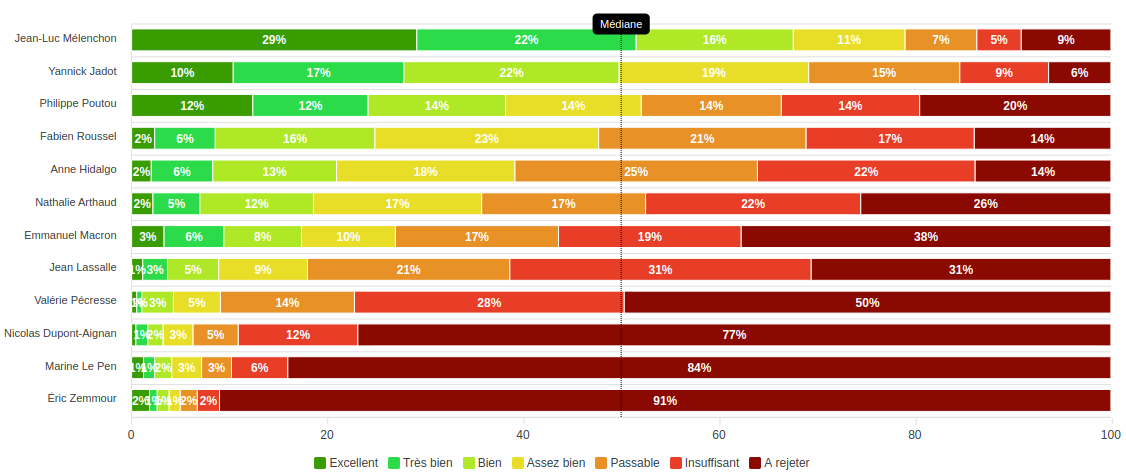
\includegraphics[scale=0.3]{data/profileUAV}
		\label{fig:distributionUAVFrench}
	\end{figure}
	
	\begin{figure}
		\centering
		\caption{Probabilité moyenne de ne pas trouver le gagnant en utilisant une distribution des préférences de cas réel, étant donné $m=12$ pour $n\in \{10,25,50,100,250,500\}$ et $k\in \intvl{1,5}$.}
		\label{fig:MJelicitationUAVFrench}
		\begin{tikzpicture}[scale=0.6]
			\pgfplotsset{
				every axis legend/.append style={
					at={(0.5,1.1)},
					anchor=south
				},
			}
			\begin{axis}[
				%	y=8,
				xlabel=$k$,
				ylabel=Avg. Prob. of Miss.,
				table/col sep=comma,
				legend columns=3,
				%	ytick={0,2,4,6,8,10},
				%	xtick distance=10,
				%	ytick distance=2,
				%	xtick pos=left,
				ymajorgrids=true,
				ytick style={draw=none},
				ymin=0,
				ymax=0.8,
				xmin=1,
				xmax=5,
				yticklabels={0,2,4,6,8,10},
				legend style={font=\scriptsize}
				]
				
				\addlegendimage{mark=halfsquare right*,brown,mark size=2}
				\addlegendimage{mark=diamond*,red,mark size=2}
				\addlegendimage{mark=pentagon*,cyan,mark size=2}
				\addlegendimage{mark=halfcircle*,violet,mark size=2}
				\addlegendimage{mark=*,pink,mark size=2}
				\addlegendimage{mark=triangle*,green,mark size=2}
				\addlegendimage{mark=halfsquare left*,blue,mark size=2}
				\addlegendimage{mark=square*,teal,mark size=2}
				\addlegendimage{mark=halfsquare*,magenta,mark size=2}
				
				
				\addplot[thick, mark=halfsquare right*, mark size = {2}, mark indices = {3}, brown] table [x=k, y=p10]{data/electiontableFig.dat};
				\addlegendentry{n=10}
				\addplot[thick, mark=diamond*, mark size = {2}, mark indices = {3}, red] table [x=k, y=p25]{data/electiontableFig.dat};
				\addlegendentry{n=25}
				\addplot[thick, mark=pentagon*, mark size = {2}, mark indices = {2}, cyan] table [x=k, y=p50]{data/electiontableFig.dat};
				\addlegendentry{n=50}
				\addplot[thick, mark=halfcircle*, mark size = {2}, mark indices = {2}, violet] table [x=k, y=p100]{data/electiontableFig.dat};
				\addlegendentry{n=100}
				\addplot[thick, mark=*, mark size = {2}, mark indices = {1}, pink] table [x=k, y=p250]{data/electiontableFig.dat};
				\addlegendentry{n=250}
				\addplot[thick, mark=triangle*, mark size = {2}, mark indices = {1}, green] table [x=k, y=p500]{data/electiontableFig.dat};
				\addlegendentry{n=500}
				%				\addplot[thick, mark=halfsquare left*, mark size = {2}, mark indices = {1}, blue] table [x=k, y=p1000]{data/electiontableFig.dat};
				%				\addlegendentry{n=1000}
				%				\addplot[thick, mark=square*, mark size = {2}, mark indices = {1}, teal] table [x=k, y=p1500]{data/electiontableFig.dat};
				%				\addlegendentry{n=1500}
				
			\end{axis}
		\end{tikzpicture}
	\end{figure}

\newpage
\section{Compromising as an equal loss principle}
	Le mot compromis vient du latin \textit{compromissus}, participe passé de \textit{compromittere} : com \textit{ensemble} et promittere \textit{promettre}.
	L'idée de compromis se retrouve en effet dans des textes datant de l'époque romaine, où deux parties en conflit qui souhaitaient soumettre leur différend à l'arbitrage désignaient un tiers (un arbitre) et promettaient mutuellement de se conformer au jugement incontestable de ce dernier. Si l'une des parties avait rompu cette promesse, elle aurait dû payer une pénalité.
	Dans un fragment d'une lettre écrite par Proculus, qui est rapporté par \citet [p.529]{Zimmermann1996}, il est clair que les deux parties au conflit ont accepté de donner à l'arbitre des pouvoirs illimités dans sa décision. Aucun recours n'était possible contre la sentence finale, qui était contraignante, aussi injuste et inégale soit-elle. Cette idée du compromis comme simple processus d'arbitrage semble très différente de la notion que nous en avons aujourd'hui. Considérons les définitions des deux verbes dans un dictionnaire moderne : arbitrer "régler un différend entre deux personnes ou groupes après avoir entendu les arguments et les opinions de chacun" ; compromettre "parvenir à un accord par concession mutuelle".
	La concession mutuelle est l'élément qui nous fait immédiatement penser à un compromis et c'est précisément le facteur manquant dans la description du compromis romain et de l'arbitrage moderne. En citant \citet{Braybrooke1982} \say{C'est tout simplement une mauvaise plaisanterie que de dire qu'une personne est partie à un compromis alors qu'elle n'en a rien retiré.}.
	
	Dans \Cref{ch:compromise}, nous présentons deux versions différentes de compromis, en particulier une qui privilégie l'égalité aux dépens de l'efficacité de Pareto. De plus, nous considérerons le concept de "equal-loss" (perte égale) \citep{Chun1988, Chun1991} comme la base du compromis dans toutes les situations où l'égalitarisme, au sens de concéder également, est une prérogative importante.
	Il s'agit d'une nouveauté dans la littérature des règles de choix social, qui jusqu'à présent n'ont fait qu'imposer la volonté de compromis sans réellement garantir que toutes les parties concèdent quelque chose.
	Le philosophe \citet{Day1989} tente d'expliquer ce phénomène en pensant qu'il découle de la négation de l'adjectif "intransigeant" : 
	\textit{\say{Une personne intransigeante est une personne qui n'est pas disposée à faire des concessions, donc (on en déduit à tort) une personne compromettante est une personne souple et disposée à faire des concessions\textemdash indépendamment du fait qu'elle reçoive une concession en retour. Quoi qu'il en soit, il faut insister, car il est généralement admis que le compromis implique nécessairement des concessions mutuelles.}}
	Cela pourrait expliquer pourquoi toutes les règles de vote qui tentent de faire un compromis se contentent en fait de la volonté des agents de faire un compromis. 
	
	\cite{Merlin2019} discutent des plus célèbres de ces procédures en proposant de les rassembler dans la même classe de \textit{règles de compromis}.
	Dans \Cref{sec:BK}, nous avons déjà défini le \acl{MC}, introduit par \citet{Sertel1986} et analysé plus en détail par \citet{Sertel1999}. Basée sur une révision de la règle de Condorcet-Bucklin, cette procédure part du choix idéal de chacun pour trouver une alternative soutenue par la majorité des votants. Si une telle alternative n'existe pas, elle se rabat sur le deuxième, le troisième et plus généralement le $k$-\emph{e} meilleur choix des votants, jusqu'à ce qu'au moins une des alternatives considérées figure parmi les $k$ premiers meilleurs pour une majorité.
	Si au lieu de considérer un accord pour la majorité des votants, nous souhaitons sélectionner comme gagnants les alternatives soutenues par l'unanimité des votants, alors la procédure correspond à la règle \acl{FB}. 
	Plus généralement, si nous considérons le soutien d'un certain quota $q$ d'électeurs, nous nous référons à la règle de "q-approval fallback bargaining" \citep{Brams2001}.
	
	Toutes ces \acp{SCR} imposent aux électeurs une volonté de compromis, mais nous soutenons qu'elles ne garantissent pas efficacement un résultat où les agents ont effectivement fait des compromis. Cet exemple motive notre point de vue:
	
	\begin{example}
		Considérons le profil de préférence suivant avec $n=100$:
		\begin{center}
			$
			\begin{array}{cc}
				\mathbf{49} & \mathbf{51} \\
				c	&	a	\\
				b	&	b	\\
				a	&	c	\\
			\end{array} \quad.
			$
		\end{center}
		Lorsque $q\in \intvl{1,\frac{n}{2}+1} $, tous les compromis BK choisissent $a$ et $c$ tandis que les compromis BK révisés choisissent $a$. Ces résultats n'apparaissent pas comme un compromis car près de la moitié des votants obtiennent leur meilleur choix tandis que l'autre moitié doit se contenter de leur pire choix. Observez que $b$ reçoit un soutien unanime lorsque chaque électeur recule d'un pas par rapport à son point idéal.
	
		When $q\in \intvl{1,\frac{n}{2}+1} $, all BK compromises pick $a$ and $c$ while the revised BK compromises select $a$. These outcomes do not appear as a compromise as almost half of the voters obtain their best choice while the remaining half have to be contented with their worst one. Observe that $b$ receives unanimous support when each voter falls back one step from her ideal point.
	\end{example}
	
	Nous définissons qu'une règle est \textit{Egalitarian Compromise} (EC) (resp., \textit{Egalitarian Compromise Compatible} (ECC)), si \emph{tous} (resp., \emph{quelques}) les gagnants sont parmi les alternatives avec les pertes les plus également distribuées. Évidemment, EC est une sous-classe de ECC.
	
	De plus, nous définissons qu'une règle est \textit{Paretian Compromise} (PC) (resp., \textit{Paretian Compromise Compatible} (PCC)), si \emph{tous} (resp., \emph{quelques}) les gagnants sont parmi les alternatives Pareto optimales avec les pertes les plus également distribuées. Évidemment, PC est une sous-classe de PCC.

	\paragraph{Conclusions.}
	Nous prouvons que : aucune procédure de Condorcet n'est ECC ou PCC (\Cref{th:condorcet}), aucune règle de score n'est ECC (\Cref{th:srECC}) ou PCC à l'exception de la règle d'antipluralité (\Cref{th:AntSatsPCC,th:srPCC}), les compromis \acs{BK} ne sont ni ECC ni PCC (\Cref{th:BKthreshold,th:FBfailsECC}) à l'exception de fallback bargaining qui est PC (\Cref{th:FBsatsPC}).
	
	Nos résultats d'impossibilité sont énoncés pour l'ensemble des mesures d'écart $\Sigma$, mais ils prévalent pour tout sous-ensemble de $\Sigma$. Comme $\Sigma$ est le plus grand ensemble de mesures d'écart sensibles, ils sont valables pour tout concept spécifique d'équité que l'on pourrait choisir. D'autre part, nos résultats de possibilité sur le fallback bargaining et l'antipluralité ne se propagent pas aux sous-ensembles de $\Sigma$. En fait, dès qu'une restriction raisonnablement légère sur $\Sigma$ est imposée, les deux règles ne sont plus PCC (\Cref{th:3votRestriction}). Avec deux individus et une restriction similaire sur $\Sigma$, tous les SCR à deux personnes bien connus de la littérature, à savoir le fallback bargaining, les règles de fallback bargaining, Pareto and veto rules, short listing et veto rank, ne parviennent pas à trouver des compromis ex-post (\Cref{th:2votPCC}).
	
	L'exclusion du principe d'égalité des pertes par la quasi-totalité de la littérature conduit à se demander si le principe ne présente pas d'intérêt dans un contexte de choix social discret. Cela semble être le cas pour les situations de vote où le nombre d'électeurs dépasse le nombre de candidats et où, en général, chaque candidat est classé dernier par au moins un électeur. Dans ces cas, la principale préoccupation concerne le soutien des alternatives plutôt que l'égalité. D'autre part, les problèmes de choix collectifs à deux personnes sont généralement interprétés comme des situations d'arbitrage ou de négociation où le consentement mutuel est un élément essentiel pour parvenir à une solution. Ainsi, le principe de perte égale semble être valide pour les problèmes de choix collectifs à deux personnes et notre analyse soulève la question de la conception de nouvelles règles d'arbitrage discrètes compatibles avec le principe de perte égale.



\end{document}
